
\documentclass[10pt,openany,a4paper]{article}
\usepackage{tikz, pgfplots, tkz-euclide,calc}
\usetikzlibrary{patterns,shapes.arrows,calc}
\usepackage{fancyhdr}
\usepackage{enumerate,enumitem}
\usepackage{cancel}
\usepackage{varwidth}

% TAMBAHKAN PACKAGE SENDIRI KALAU KURANG

\usepackage{geometry}
\geometry{
	left = 22mm,
	right = 22mm,
	top = 25mm,
	bottom = 25mm,
}
\usepackage{graphicx}
\usepackage{subcaption}
\usepackage{soul}
\usepackage{hyperref}
\usepackage{float}
\usepackage{setspace}
\usepackage{afterpage}
\usepackage{xcolor}
\usepackage[nosectionbib]{apacite}
\usepackage{lmodern}
\usepackage{mathtools}
\usepackage{upgreek}
\usepackage{siunitx}
% \usepackage{fontawesome5}
\usepackage{fontawesome6}
\usepackage{physics}
\usepackage{pdfpages}
\usepackage{hyperref}
\renewcommand{\baselinestretch}{1.3}
\usepackage{multicol}
\usepackage{hyperref,ragged2e,amsmath,multicol,gensymb,setspace,
fancyhdr,amsfonts,tikz,pgfplots,nccmath,enumerate,verbatim,amsthm,physics}
\usepgfplotslibrary{polar,fillbetween}
% Disable tikz externalization to avoid requiring -shell-escape
\usepgfplotslibrary{external}
\tikzexternalize[prefix=tikz/]
\tikzset{reuse path/.code={\pgfsyssoftpath@setcurrentpath{#1}}}
\usetikzlibrary{shapes.geometric,arrows}
\newcommand\mylog[1]{\mathop{{}^{#1}\mathrm{log}}}
\pgfplotsset{compat=1.15}
\pgfplotsset{my style/.append style={axis x line=middle, axis y line=
middle, xlabel={$x$}, ylabel={$y$}, axis equal }}
\usepackage{etoolbox}
% remove stray \makeatother
\newtheorem{defn}{Definisi}[section]
\newtheorem{teo}[defn]{Teorema}
\newtheorem{thm}{Teorema}[section]
\newtheorem{lemma}{Lemma}
\newtheorem{lemmas}[defn]{Lemma}
\newtheorem{cor}[defn]{Akibat}
\newtheorem{asumsi}[defn]{Asumsi}
\theoremstyle{definition}
\newtheorem{con}{Contoh}[section]
\theoremstyle{definition}
\theoremstyle{plain}
\newtheorem{prop}{Proposisi}[section]
\renewcommand{\proofname}{Bukti}
\renewcommand{\thethm}{\arabic{chapter}.\arabic{thm}}

\newcommand{\normlp}[1]{\left\|#1\right\|_{L^p_{\lambda}(0,T;H)}}% Fungsi norm (||x||)
\newcommand{\R}{\mathbb{R}}
\renewcommand{\natural}{\mathbb{N}}
\newcommand{\Xpl}{X^R_{p,\lambda}}
\newcommand{\Xpls}{X^R_{p,\lambda^*}}
\newcommand{\qpl}{q^R_{p,\lambda}}
\newcommand{\qpls}{q^R_{p,\lambda^*}}
\pagestyle{fancy}
\fancyhf{}
\lhead{Halaman \thepage}
% \cfoot{\faXTwitter\ \href{https://x.com/ahmadzakiyudin_/}{@ahmadzakiyudin\_} | \faInstagram\ \href{https://instagram.com/ahmadzakiyudin_/}{@ahmadzakiyudin\_} | \faTiktok\ \href{https://tiktok.com/@ahmathz/}{@ahmathz}}
% \rhead{Pembahasan Soal ETS \\ Kalkulus 1 ITS 2025/2026}
\hypersetup{
    colorlinks=true,
    linkcolor=blue,
    filecolor=blue,      
    urlcolor=blue,
}
\newenvironment{jawab}[2][tes]{%
% \fbox{\begin{minipage}{14.65cm}
% \par + \noindent: selalu mulai di baris baru tanpa menjorok,
% termasuk setelah display math (align, \[ \]) di akhir soal
\par\noindent\textbf{Kata kunci materi:} #1.\\
\textbf{Penyelesaian:} #2%
% \end{minipage}}
}{}

\newenvironment{jawab2}[2][tes]{
\fbox{\begin{minipage}{14.65cm}
 #2
\end{minipage}}}{}

\newenvironment{jawaban}[2][tes]{
\colorlet{oldcolor}{.}
        \color{red}
        \setlength{\fboxrule}{1pt}\boxed{\color{oldcolor}#2}\color{oldcolor}.
}{}

\newenvironment{jawaban2}[2][tes]{
\colorlet{oldcolor}{.}
        \color{red}
        \setlength{\fboxrule}{1pt}\fbox{\color{oldcolor}#2}\color{oldcolor}.
}{}

\newenvironment{penting}[2][tes]{
\colorlet{oldcolor}{.}
\color{blue}
\fbox{\color{oldcolor}#2}\color{oldcolor}
}{}

\begin{document}
% \begin{titlepage}
%     \vspace*{\fill}
%     \begin{center}
%       \Huge {PEMBAHASAN SOAL EAS \\ KALKULUS II \\ TAHUN 2024/2025}\\[0.4 cm]
%       \huge {Ahmad Hisbu Zakiyudin}\\[0.2 cm]
%       \Large {(\href{https://instagram.com/ahmadzakiyudin_/}{@ahmadzakiyudin\_})}
%     \end{center}
%     \vspace*{\fill}
%   \end{titlepage}
% !TEX root = ../../BookTemplate.tex
%%%%%%%%%%%%%%%%%%%%%%%%%%%%%%%%%%%%%%%%%%%%%%%%%%%%%%%%%%%%%%%%%%%%%%%%%%%%%%%%%%
% \begin{titlepage}
%     \raggedleft	
% 	\hspace{.025\textwidth}
% 	\parbox[b]{\textwidth}{
%     \vspace{1.5cm}
% 		{\Huge\bfseries Pembahasan Soal EAS}                \\[20pt]
% 		{\huge\textit\ Kalkulus II}\\ \\[10pt]
%         {\Large\textsc{Tahun 2024/2025}}}
% \vfill
% \rule{1pt}{.14\textheight}
% \hspace{.025\textwidth}
%     \raisebox{10pt}{\parbox[b]{.95\textwidth}{ 
%         {\Large\textsc{Ahmad Hisbu Zakiyudin}}              \\[10pt]
%         \large{\href{https://instagram.com/ahmadzakiyudin_/}{@ahmadzakiyudin\_}}               \\[25pt]
%         {\large 5 Juni 2026}}}
% \end{titlepage}
\begin{titlepage}
	\centering % Center everything on the title page
	% \scshape % Use small caps for all text on the title page
	\vspace*{1.5\baselineskip} % White space at the top of the page
% ===================
%	Title Section 	
% ===================

	\rule{13cm}{1.6pt}\vspace*{-\baselineskip}\vspace*{2pt} % Thick horizontal rule
	\rule{13cm}{0.4pt} % Thin horizontal rule
	
		\vspace{0.75\baselineskip} % Whitespace above the title
% ========== Title ===============	
	{	\Huge Pembahasan Soal\\ 
			\vspace{4mm}
		Tryout ETS Kalkulus 1 \\ \vspace{2mm} \huge{Tahun 2026/2027}\\	}
% ======================================
		\vspace{0.75\baselineskip} % Whitespace below the title
	\rule{13cm}{0.4pt}\vspace*{-\baselineskip}\vspace{3.2pt} % Thin horizontal rule
	\rule{13cm}{1.6pt} % Thick horizontal rule
	
		\vspace{1.75\baselineskip} % Whitespace after the title block
% =================
%	Information	
% =================
{\large Oleh: Ahmad Hisbu Zakiyudin}
	% {\large Oleh: Ahmad Hisbu Zakiyudin \\
	% 	\vspace*{1.2\baselineskip}
	% \href{https://instagram.com/ahmadzakiyudin_/}{@ahmadzakiyudin\_}} \\
	\vfill
	\vspace{1mm}
\huge{Selamat Belajar!}
\end{titlepage}
\makeatletter
\setlength\fboxsep{3pt}
% ensure enough header height for fancyhdr
\setlength{\headheight}{24pt}
% Kop tiap kelompok: #1 kelompok, #2 kelas, #3 departemen, #4 jadwal kuliah, #5 sesi
\newcommand{\kopsoal}[5]{%
 \begin{center}
	{\underline{\textbf{\MakeUppercase{Soal dan Pembahasan Tryout ETS Kalkulus 1 Tahun 2026/2027}}}}
    \end{center}

    \begin{center}
	\begin{tabular}{lcl}
		Mata kuliah/SKS & : & Kalkulus 1 ( SM234101 ) / 3 SKS\\
		Kelompok & : & #1\\
		Kelas & : & #2\\
		Departemen & : & #3\\
		Jadwal kuliah & : & #4\\
		Sesi & : & #5\\
		Waktu & : & 100 menit\\
		Sifat & : & Tertutup\\
  ~
	\end{tabular}

    \noindent\rule{\textwidth}{2.pt}
        \end{center}}

% Kop kelompok IUP (bahasa Inggris): #1 kelompok, #2 kelas, #3 departemen, #4 jadwal kuliah, #5 sesi
\newcommand{\kopsoaliup}[5]{%
 \begin{center}
	{\underline{\textbf{\MakeUppercase{Soal dan Pembahasan Tryout ETS Kalkulus 1 Tahun 2026/2027}}}}
    \end{center}

    \begin{center}
	\begin{tabular}{lcl}
		Course / Credit & : & Kalkulus 1 ( SM234101 ) / 3 SKS\\
		Group & : & #1\\
		Class & : & #2\\
		Department & : & #3\\
		Lecture schedule & : & #4\\
		Session & : & #5\\
		Time & : & 100 minutes\\
		Type & : & Closed\\
  ~
	\end{tabular}

    \noindent\rule{\textwidth}{2.pt}
        \end{center}}

% Kop tryout Matematika 2 SKS: #1 kelompok, #2 kelas, #3 departemen, #4 jadwal kuliah, #5 sesi
\newcommand{\kopsoalmat}[5]{%
 \begin{center}
	{\underline{\textbf{\MakeUppercase{Soal dan Pembahasan Tryout ETS Matematika Tahun 2026/2027}}}}
    \end{center}

    \begin{center}
	\begin{tabular}{lcl}
		Mata kuliah/SKS & : & Matematika ( SM234152 ) / 2 SKS\\
		Kelompok & : & #1\\
		Kelas & : & #2\\
		Departemen & : & #3\\
		Jadwal kuliah & : & #4\\
		Sesi & : & #5\\
		Waktu & : & 100 menit\\
		Sifat & : & Tertutup\\
  ~
	\end{tabular}

    \noindent\rule{\textwidth}{2.pt}
        \end{center}}

% Kop tryout Matematika 2 SKS IUP (bahasa Inggris)
\newcommand{\kopsoalmatiup}[5]{%
 \begin{center}
	{\underline{\textbf{\MakeUppercase{Soal dan Pembahasan Tryout ETS Matematika Tahun 2026/2027}}}}
    \end{center}

    \begin{center}
	\begin{tabular}{lcl}
		Course / Credit & : & Matematika ( SM234152 ) / 2 SKS\\
		Group & : & #1\\
		Class & : & #2\\
		Department & : & #3\\
		Lecture schedule & : & #4\\
		Session & : & #5\\
		Time & : & 100 minutes\\
		Type & : & Closed\\
  ~
	\end{tabular}

    \noindent\rule{\textwidth}{2.pt}
        \end{center}}


%%%%%%%%%%%%%%%%%%%%%%%%%%%%%%%%%%%%%%%%%%%%%%%%%%%%%%%%%%%%%%%%%%%%%%%%%%%%%%
% Kal-5
% Kisi-kisi hari Senin: subbab 1.1, 1.5, 2.3, 2.4, 3.1, 3.3, 4.2, 4.4
\kopsoal{Kal-5}{22-27}{T. Fisika, T. Material dan Metalurgi, Rkp}{Senin, Rabu; 07.00-09.30}{1}
\begin{enumerate}
    \item \textbf{[Subbab 1.1]} Dapatkan himpunan penyelesaian pertidaksamaan
    \begin{align*}
        3\leq\frac{x^2+2}{x}<x+2
    \end{align*}
    \begin{jawab}[pertidaksamaan rasional, pertidaksamaan ganda, garis bilangan, irisan himpunan]{~\\
        Pertidaksamaan ganda tersebut dapat dipecah menjadi dua pertidaksamaan yang harus dipenuhi sekaligus, yaitu
        \begin{align*}
            \colorlet{oldcolor}{.}
        \color{blue}
        \setlength{\fboxrule}{1pt} \boxed{\color{oldcolor}3\leq\frac{x^2+2}{x}}\color{oldcolor} \quad\text{dan}\quad \colorlet{oldcolor}{.}
        \color{blue}
        \setlength{\fboxrule}{1pt} \boxed{\color{oldcolor}\frac{x^2+2}{x}<x+2}\color{oldcolor}.
        \end{align*}
        Diperhatikan bahwa $x\neq 0$ karena $x$ berada pada penyebut.
        \begin{enumerate}
            \item[(i)] Untuk $3\leq\frac{x^2+2}{x}$, pindahkan semua suku ke ruas kiri sehingga ruas kanan bernilai nol:
            \begin{align*}
                \frac{x^2+2}{x}-3 &\geq 0\\
                \frac{x^2+2-3x}{x} &\geq 0\\
                \frac{(x-1)(x-2)}{x} &\geq 0.
            \end{align*}
            Pembuat nolnya adalah $x=0$, $x=1$, dan $x=2$. Dengan uji titik, misalkan $x=-1$ diperoleh $\frac{(-2)(-3)}{-1}<0$, $x=\frac{1}{2}$ diperoleh $\frac{(-\frac{1}{2})(-\frac{3}{2})}{\frac{1}{2}}>0$, $x=\frac{3}{2}$ diperoleh $\frac{(\frac{1}{2})(-\frac{1}{2})}{\frac{3}{2}}<0$, dan $x=3$ diperoleh $\frac{(2)(1)}{3}>0$.
            \begin{center}
                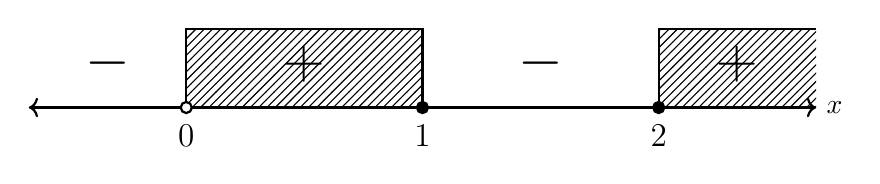
\begin{tikzpicture}
    \draw[thick,<->] (-5,0) -- (5,0) node[right] {$x$};
    \fill[pattern=north east lines] (-3,0) rectangle (0,1);
    \fill[pattern=north east lines] (3,0) rectangle (5,1);
    \draw[thick] (-3,0) -- (-3,1) -- (0,1) -- (0,0);
    \draw[thick] (3,0) -- (3,1) -- (5,1);
    \draw (-3,-0.1) node[below] {\large{$0$}};
    \draw (0,-0.1) node[below] {\large{$1$}};
    \draw (3,-0.1) node[below] {\large{$2$}};
    \draw (-4,0.2) node[above] {\huge{$-$}};
    \draw (-1.5,0.2) node[above] {\huge{$+$}};
    \draw (1.5,0.2) node[above] {\huge{$-$}};
    \draw (4,0.2) node[above] {\huge{$+$}};
    \draw[fill=white, thick] (-3,0) circle (2pt);
    \draw[fill=black, thick] (0,0) circle (2pt);
    \draw[fill=black, thick] (3,0) circle (2pt);
                \end{tikzpicture}
            \end{center}
            Karena yang diminta lebih dari atau sama dengan nol, diperoleh $\colorlet{oldcolor}{.}
        \color{blue}
        \setlength{\fboxrule}{1pt} \boxed{\color{oldcolor}HP_1=(0,1]\cup[2,\infty)}\color{oldcolor}$.
            \item[(ii)] Untuk $\frac{x^2+2}{x}<x+2$, dengan cara yang sama diperoleh
            \begin{align*}
                \frac{x^2+2}{x}-(x+2) &< 0\\
                \frac{x^2+2-x^2-2x}{x} &< 0\\
                \frac{2(1-x)}{x} &< 0.
            \end{align*}
            Pembuat nolnya adalah $x=0$ dan $x=1$. Dengan uji titik, misalkan $x=-1$ diperoleh $\frac{2(2)}{-1}<0$, $x=\frac{1}{2}$ diperoleh $\frac{2(\frac{1}{2})}{\frac{1}{2}}>0$, dan $x=2$ diperoleh $\frac{2(-1)}{2}<0$.
            \begin{center}
                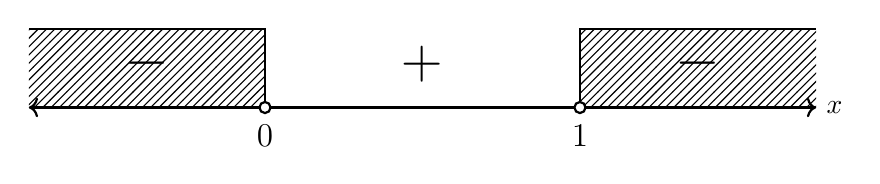
\begin{tikzpicture}
    \draw[thick,<->] (-5,0) -- (5,0) node[right] {$x$};
    \fill[pattern=north east lines] (-5,0) rectangle (-2,1);
    \fill[pattern=north east lines] (2,0) rectangle (5,1);
    \draw[thick] (-5,1) -- (-2,1) -- (-2,0);
    \draw[thick] (2,0) -- (2,1) -- (5,1);
    \draw (-2,-0.1) node[below] {\large{$0$}};
    \draw (2,-0.1) node[below] {\large{$1$}};
    \draw (-3.5,0.2) node[above] {\huge{$-$}};
    \draw (0,0.2) node[above] {\huge{$+$}};
    \draw (3.5,0.2) node[above] {\huge{$-$}};
    \draw[fill=white, thick] (-2,0) circle (2pt);
    \draw[fill=white, thick] (2,0) circle (2pt);
                \end{tikzpicture}
            \end{center}
            Karena yang diminta kurang dari nol, diperoleh $\colorlet{oldcolor}{.}
        \color{blue}
        \setlength{\fboxrule}{1pt} \boxed{\color{oldcolor}HP_2=(-\infty,0)\cup(1,\infty)}\color{oldcolor}$.
        \end{enumerate}
        Himpunan penyelesaian pertidaksamaan ganda adalah irisan dari kedua himpunan tersebut, yaitu
        \begin{align*}
            HP_1\cap HP_2 = \big((0,1]\cup[2,\infty)\big)\cap\big((-\infty,0)\cup(1,\infty)\big) = [2,\infty).
        \end{align*}
        Sebagai pengecekan, untuk $x=2$ diperoleh $\frac{4+2}{2}=3$, dan berlaku $3\leq 3<4$. Jadi himpunan penyelesaiannya adalah $\colorlet{oldcolor}{.}
        \color{red}
        \setlength{\fboxrule}{1pt} \boxed{\color{oldcolor}\{x\in\mathbb{R} : x\geq 2\}=[2,\infty)}\color{oldcolor}$.
    }
    \end{jawab}

    \item \textbf{[Subbab 1.5]} Diberikan lingkaran $x^2+y^2-6x-8y=0$.
    \begin{enumerate}
        \item Dapatkan pusat dan jari-jari lingkaran tersebut.
        \item Tentukan titik-titik potong lingkaran dengan sumbu-$x$ dan sumbu-$y$.
        \item Sketsa grafik lingkaran tersebut.
    \end{enumerate}
    \begin{jawab}[persamaan lingkaran, melengkapkan kuadrat, titik potong sumbu, sketsa grafik]{
        \begin{enumerate}
            \item Persamaan lingkaran diubah ke bentuk baku $(x-a)^2+(y-b)^2=r^2$ dengan cara melengkapkan kuadrat, yaitu
            \begin{align*}
                x^2-6x+y^2-8y &= 0\\
                (x^2-6x+9)+(y^2-8y+16) &= 9+16\\
                (x-3)^2+(y-4)^2 &= 25.
            \end{align*}
            Jadi pusat dan jari-jari lingkaran adalah $\colorlet{oldcolor}{.}
        \color{red}
        \setlength{\fboxrule}{1pt} \boxed{\color{oldcolor}\text{Pusat: }(3,4),~\text{Jari-jari: }5}\color{oldcolor}$.
            \item Titik potong dengan sumbu-$x$ diperoleh dengan substitusi $y=0$ ke persamaan lingkaran, yaitu
            \begin{align*}
                x^2-6x=0 \iff x(x-6)=0 \iff x=0 \;\vee\; x=6,
            \end{align*}
            sehingga titik potongnya adalah $\colorlet{oldcolor}{.}
        \color{blue}
        \setlength{\fboxrule}{1pt} \boxed{\color{oldcolor}(0,0)}\color{oldcolor}$ dan $\colorlet{oldcolor}{.}
        \color{blue}
        \setlength{\fboxrule}{1pt} \boxed{\color{oldcolor}(6,0)}\color{oldcolor}$. Titik potong dengan sumbu-$y$ diperoleh dengan substitusi $x=0$, yaitu
            \begin{align*}
                y^2-8y=0 \iff y(y-8)=0 \iff y=0 \;\vee\; y=8,
            \end{align*}
            sehingga titik potongnya adalah $\colorlet{oldcolor}{.}
        \color{blue}
        \setlength{\fboxrule}{1pt} \boxed{\color{oldcolor}(0,0)}\color{oldcolor}$ dan $\colorlet{oldcolor}{.}
        \color{blue}
        \setlength{\fboxrule}{1pt} \boxed{\color{oldcolor}(0,8)}\color{oldcolor}$. Jadi titik-titik potong lingkaran dengan sumbu koordinat adalah $\colorlet{oldcolor}{.}
        \color{red}
        \setlength{\fboxrule}{1pt} \boxed{\color{oldcolor}(0,0),~(6,0),~\text{dan }(0,8)}\color{oldcolor}$. Diperhatikan bahwa lingkaran melalui titik asal karena $0^2+0^2-6(0)-8(0)=0$.
            \item Sketsa lingkaran dengan pusat $(3,4)$ dan jari-jari $5$ adalah sebagai berikut:
            \begin{center}
                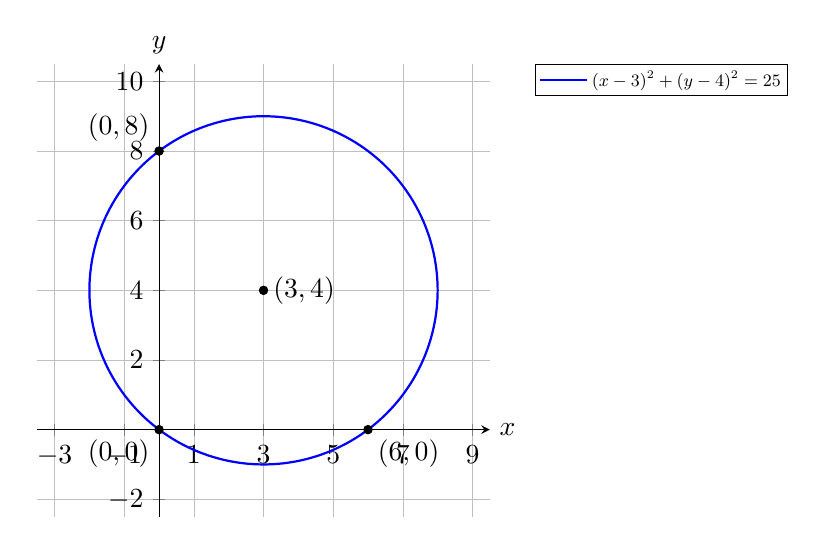
\begin{tikzpicture}
                    \begin{axis}[
        axis lines = middle,
        xlabel = $x$,
        ylabel = {$y$},
        grid=both,
        grid style={line width=.1pt, draw=gray!10},
        major grid style={line width=.2pt,draw=gray!50},
        x label style={anchor=west}, % label x ke kanan
        y label style={anchor=south}, % label y ke atas
        samples=200,
        legend style={
                at={(1.1,1)},
                anchor=north west,
                font=\small,         % mengecilkan ukuran font
                row sep=1pt,         % jarak antar baris legend
                inner sep=1pt,       % margin dalam kotak legend
                nodes={scale=0.7}    % skalakan isi legend
            },
        xtick={-3,-1,...,9},
        ytick={-2,0,...,10},
        xmin=-3.5, xmax=9.5,
        ymin=-2.5, ymax=10.5,
        axis equal image,
        width=8.5cm
    ]
\addplot[domain=0:360, color=blue, thick] ({3+5*cos(x)}, {4+5*sin(x)});
\addlegendentry{$(x-3)^2+(y-4)^2=25$}
\draw[fill=black] (3,4) circle (1.5pt) node[right] {$(3,4)$};
\draw[fill=black] (0,0) circle (1.5pt) node[below left] {$(0,0)$};
\draw[fill=black] (6,0) circle (1.5pt) node[below right] {$(6,0)$};
\draw[fill=black] (0,8) circle (1.5pt) node[above left] {$(0,8)$};
\end{axis}
                \end{tikzpicture}
            \end{center}
        \end{enumerate}
    }
    \end{jawab}

    \item \textbf{[Subbab 2.4]} Diberikan suatu fungsi $f(x)=1+\sqrt{4-x^2}$ dengan domain $f$ adalah $[a,2]$.
    \begin{enumerate}
        \item Tentukan nilai terkecil $a$ agar $f^{-1}(x)$ ada.
        \item Dapatkan $f^{-1}(x)$.
        \item Dapatkan domain dan range dari $f^{-1}(x)$.
    \end{enumerate}
    \begin{jawab}[fungsi satu-satu, setengah lingkaran, fungsi invers, domain dan range]{
        \begin{enumerate}
            \item Suatu fungsi mempunyai invers jika fungsi tersebut satu-satu (injektif). Diperhatikan bahwa jika $y=1+\sqrt{4-x^2}$, maka $y-1=\sqrt{4-x^2}\geq 0$ dan
            \begin{align*}
                (y-1)^2 = 4-x^2 \iff \colorlet{oldcolor}{.}
        \color{blue}
        \setlength{\fboxrule}{1pt} \boxed{\color{oldcolor}x^2+(y-1)^2=4}\color{oldcolor},\quad y\geq 1,
            \end{align*}
            sehingga grafik $f$ adalah setengah lingkaran bagian atas dengan pusat $(0,1)$ dan jari-jari $2$. Grafik ini naik pada $[-2,0]$ dan turun pada $[0,2]$, sehingga jika domainnya memuat titik di kiri dan kanan $x=0$, fungsi $f$ tidak satu-satu (misalnya $f(-1)=f(1)=1+\sqrt{3}$). Agar $f$ satu-satu pada $[a,2]$, haruslah $a\geq 0$. Jadi nilai terkecil $a$ adalah $\colorlet{oldcolor}{.}
        \color{red}
        \setlength{\fboxrule}{1pt} \boxed{\color{oldcolor}a=0}\color{oldcolor}$.
            \item Misalkan $y=f(x)$ dengan $x\in[0,2]$, kemudian selesaikan sehingga terbentuk $x$ dalam fungsi $y$. Diperoleh
            \begin{align*}
                y &= 1+\sqrt{4-x^2}\\
                y-1 &= \sqrt{4-x^2}\\
                (y-1)^2 &= 4-x^2\\
                x^2 &= 4-(y-1)^2\\
                x &= \sqrt{4-(y-1)^2} \quad (\text{karena } x\geq 0).
            \end{align*}
            Dari sini didapatkan $x = f^{-1}(y) = \sqrt{4-(y-1)^2}$. Dengan mengganti $y$ dengan $x$, diperoleh
            \begin{align*}
                \colorlet{oldcolor}{.}
        \color{red}
        \setlength{\fboxrule}{1pt} \boxed{\color{oldcolor}f^{-1}(x) = \sqrt{4-(x-1)^2} = \sqrt{3+2x-x^2}}\color{oldcolor}.
            \end{align*}
            \item Pada domain $[0,2]$, fungsi $f$ turun dari $f(0)=1+\sqrt{4}=3$ sampai $f(2)=1+\sqrt{0}=1$, sehingga range dari $f$ adalah $R(f)=[1,3]$. Domain dari fungsi invers adalah range dari fungsi asli dan range dari fungsi invers adalah domain dari fungsi asli, yaitu
            \begin{align*}
                \colorlet{oldcolor}{.}
        \color{red}
        \setlength{\fboxrule}{1pt} \boxed{\color{oldcolor}D(f^{-1}) = R(f) = [1, 3]}\color{oldcolor} \quad\text{dan}\quad \colorlet{oldcolor}{.}
        \color{red}
        \setlength{\fboxrule}{1pt} \boxed{\color{oldcolor}R(f^{-1}) = D(f) = [0, 2]}\color{oldcolor}.
            \end{align*}
        \end{enumerate}
    }
    \end{jawab}

    \item \textbf{[Subbab 3.1]} Diberikan $f(x)=\begin{cases}
        x+3, & x<-1\\
        x^2, & x\geq -1
    \end{cases}$.
    \begin{enumerate}
        \item Sketsa grafik $f$.
        \item Dapatkan $\displaystyle\lim_{x\to-1^-}f(x)$, $\displaystyle\lim_{x\to-1^+}f(x)$, dan $\displaystyle\lim_{x\to 2}f(x)$. Apakah $\displaystyle\lim_{x\to-1}f(x)$ ada?
    \end{enumerate}
    \begin{jawab}[fungsi sepotong-sepotong, sketsa grafik, limit sepihak]{
        \begin{enumerate}
            \item Grafik $f$ terdiri dari dua potongan, yaitu garis $y=x+3$ untuk $x<-1$ (berakhir di titik $(-1,2)$ yang tidak termasuk grafik) dan parabola $y=x^2$ untuk $x\geq -1$ (dimulai dari titik $(-1,1)$ yang termasuk grafik). Sketsa grafiknya adalah sebagai berikut:
            \begin{center}
                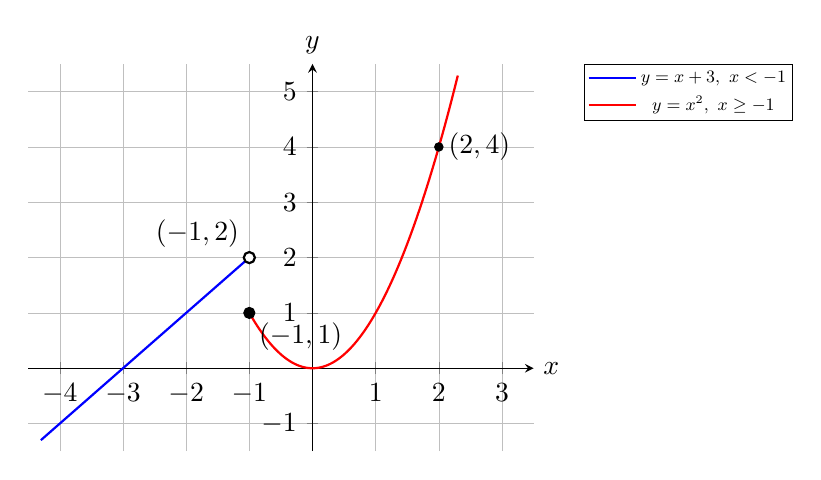
\begin{tikzpicture}
                    \begin{axis}[
        axis lines = middle,
        xlabel = $x$,
        ylabel = {$y$},
        grid=both,
        grid style={line width=.1pt, draw=gray!10},
        major grid style={line width=.2pt,draw=gray!50},
        x label style={anchor=west}, % label x ke kanan
        y label style={anchor=south}, % label y ke atas
        samples=200,
        legend style={
                at={(1.1,1)},
                anchor=north west,
                font=\small,         % mengecilkan ukuran font
                row sep=1pt,         % jarak antar baris legend
                inner sep=1pt,       % margin dalam kotak legend
                nodes={scale=0.7}    % skalakan isi legend
            },
        xtick={-4,-3,...,3},
        ytick={-1,0,...,5},
        xmin=-4.5, xmax=3.5,
        ymin=-1.5, ymax=5.5,
        width=8cm,
        height=6.5cm
    ]
\addplot[domain=-4.3:-1, color=blue, thick, samples=2] {x+3};
\addlegendentry{$y=x+3,\ x<-1$}
\addplot[domain=-1:2.3, color=red, thick] {x^2};
\addlegendentry{$y=x^2,\ x\geq -1$}
\draw[fill=white, thick] (-1,2) circle (2pt) node[above left] {$(-1,2)$};
\draw[fill=black] (-1,1) circle (2pt) node[below right] {$(-1,1)$};
\draw[fill=black] (2,4) circle (1.5pt) node[right] {$(2,4)$};
\end{axis}
                \end{tikzpicture}
            \end{center}
            \item Untuk $x\to -1^-$ (yaitu $x<-1$) digunakan rumus $x+3$, sedangkan untuk $x\to -1^+$ (yaitu $x>-1$) digunakan rumus $x^2$. Diperoleh
            \begin{align*}
                \lim_{x\to -1^-} f(x) = \lim_{x\to -1^-} (x+3) = \colorlet{oldcolor}{.}
        \color{red}
        \setlength{\fboxrule}{1pt} \boxed{\color{oldcolor}2}\color{oldcolor} \quad\text{dan}\quad \lim_{x\to -1^+} f(x) = \lim_{x\to -1^+} x^2 = \colorlet{oldcolor}{.}
        \color{red}
        \setlength{\fboxrule}{1pt} \boxed{\color{oldcolor}1}\color{oldcolor}.
            \end{align*}
            Ingat kembali bahwa $\displaystyle\lim_{x\to a}f(x)$ ada jika dan hanya jika $\colorlet{oldcolor}{.}
        \color{blue}
        \setlength{\fboxrule}{1pt} \boxed{\color{oldcolor}\lim_{x \to a^-} f(x) = \lim_{x \to a^+} f(x)}\color{oldcolor}$. Karena $2\neq 1$, maka $\colorlet{oldcolor}{.}
        \color{red}
        \setlength{\fboxrule}{1pt} \boxed{\color{oldcolor}\lim_{x\to -1}f(x) \text{ tidak ada}}\color{oldcolor}$.\\
            Selanjutnya, di sekitar $x=2$ (baik dari kiri maupun dari kanan) berlaku $x>-1$, sehingga digunakan rumus $x^2$ pada kedua sisi. Diperoleh
            \begin{align*}
                \lim_{x\to 2} f(x) = \lim_{x\to 2} x^2 = \colorlet{oldcolor}{.}
        \color{red}
        \setlength{\fboxrule}{1pt} \boxed{\color{oldcolor}4}\color{oldcolor}.
            \end{align*}
            Hal ini juga terlihat pada grafik, yaitu di $x=-1$ grafik ``meloncat'', sedangkan di sekitar $x=2$ grafik menyambung.
        \end{enumerate}
    }
    \end{jawab}

    \item \textbf{[Subbab 4.4]} Diberikan fungsi implisit $x^2+2y^2-3xy+2x-y=3$.
    \begin{enumerate}
        \item Tentukan $\dfrac{dy}{dx}$ di titik $(2,1)$.
        \item Dapatkan persamaan garis singgung kurva di titik tersebut.
    \end{enumerate}
    \begin{jawab}[diferensiasi implisit, aturan perkalian, aturan rantai, persamaan garis singgung]{
        \begin{enumerate}
            \item Kita turunkan kedua ruas persamaan terhadap $x$, dengan mengingat bahwa $y$ adalah fungsi dari $x$ (yaitu $y=y(x)$). Dengan aturan rantai, $\colorlet{oldcolor}{.}
        \color{blue}
        \setlength{\fboxrule}{1pt} \boxed{\color{oldcolor}\frac{d}{dx}(2y^2) = 4y\frac{dy}{dx}}\color{oldcolor}$, dan dengan aturan perkalian, $\colorlet{oldcolor}{.}
        \color{blue}
        \setlength{\fboxrule}{1pt} \boxed{\color{oldcolor}\frac{d}{dx}(3xy) = 3y + 3x\frac{dy}{dx}}\color{oldcolor}$. Diperoleh
            \begin{align*}
                \frac{d}{dx}(x^2) + \frac{d}{dx}(2y^2) - \frac{d}{dx}(3xy) + \frac{d}{dx}(2x) - \frac{d}{dx}(y) &= \frac{d}{dx}(3)\\
                2x + 4y\frac{dy}{dx} - 3y - 3x\frac{dy}{dx} + 2 - \frac{dy}{dx} &= 0.
            \end{align*}
            Selanjutnya, kumpulkan semua suku yang mengandung $\frac{dy}{dx}$ di satu ruas:
            \begin{align*}
                (4y - 3x - 1)\frac{dy}{dx} &= 3y - 2x - 2\\
                \frac{dy}{dx} &= \colorlet{oldcolor}{.}
        \color{blue}
        \setlength{\fboxrule}{1pt} \boxed{\color{oldcolor}\frac{3y - 2x - 2}{4y - 3x - 1}}\color{oldcolor}.
            \end{align*}
            Terlebih dahulu dicek bahwa titik $(2,1)$ terletak pada kurva, yaitu $2^2+2(1)^2-3(2)(1)+2(2)-1=4+2-6+4-1=3$. Selanjutnya, substitusi titik $(2,1)$ ke dalam turunan:
            \begin{align*}
                \frac{dy}{dx}\bigg|_{(2,1)} = \frac{3(1) - 2(2) - 2}{4(1) - 3(2) - 1} = \frac{-3}{-3} = \colorlet{oldcolor}{.}
        \color{red}
        \setlength{\fboxrule}{1pt} \boxed{\color{oldcolor}1}\color{oldcolor}.
            \end{align*}
            \item Gradien garis singgung di titik $(2,1)$ adalah $m=1$. Dengan menggunakan persamaan garis $y - y_1 = m(x - x_1)$, di mana $(x_1,y_1)=(2,1)$, diperoleh
            \begin{align*}
                y - 1 &= 1(x - 2)\\
                y &= x - 1.
            \end{align*}
            Jadi persamaan garis singgung di titik $(2,1)$ adalah $\colorlet{oldcolor}{.}
        \color{red}
        \setlength{\fboxrule}{1pt} \boxed{\color{oldcolor}y = x - 1}\color{oldcolor}$.
        \end{enumerate}
    }
    \end{jawab}
\end{enumerate}

\newpage

%%%%%%%%%%%%%%%%%%%%%%%%%%%%%%%%%%%%%%%%%%%%%%%%%%%%%%%%%%%%%%%%%%%%%%%%%%%%%%
% Kal-6
% Kisi-kisi hari Senin: subbab 1.1, 1.5, 2.3, 2.4, 3.1, 3.3, 4.2, 4.4
\kopsoal{Kal-6}{28-31}{T. Perkapalan, T. Transportasi Laut, T. Bangunan Lepas Pantai}{Senin, Rabu; 07.00-09.30}{1}
\begin{enumerate}
    \item \textbf{[Subbab 1.1]} Selesaikan pertidaksamaan berikut
    \begin{align*}
        \frac{x+2}{1-x}\geq\frac{x}{x+4}.
    \end{align*}
    \begin{jawab}[pertidaksamaan rasional, definit positif, garis bilangan, notasi interval]{~\\
        Untuk menyelesaikan pertidaksamaan rasional, pastikan ruas kanan sudah bernilai nol (jangan dikali silang, karena tanda penyebutnya belum diketahui). Diperoleh
        \begin{align*}
            \frac{x+2}{1-x}-\frac{x}{x+4} &\geq 0\\
            \frac{(x+2)(x+4)-x(1-x)}{(1-x)(x+4)} &\geq 0\\
            \frac{x^2+6x+8-x+x^2}{(1-x)(x+4)} &\geq 0\\
            \frac{2x^2+5x+8}{(1-x)(x+4)} &\geq 0.
        \end{align*}
        Diperhatikan bahwa pembilang $2x^2+5x+8$ memiliki diskriminan $D=5^2-4(2)(8)=-39<0$ dan koefisien $x^2$ positif, sehingga $\colorlet{oldcolor}{.}
        \color{blue}
        \setlength{\fboxrule}{1pt} \boxed{\color{oldcolor}2x^2+5x+8>0 \text{ untuk setiap } x}\color{oldcolor}$ (definit positif). Akibatnya, pembilang tidak pernah nol dan tanda ekspresi hanya ditentukan oleh penyebutnya, yaitu
        \begin{align*}
            \frac{2x^2+5x+8}{(1-x)(x+4)}\geq 0 \iff (1-x)(x+4)>0.
        \end{align*}
        Pembuat nol penyebut adalah $\colorlet{oldcolor}{.}
        \color{blue}
        \setlength{\fboxrule}{1pt} \boxed{\color{oldcolor}x=-4}\color{oldcolor}$ dan $\colorlet{oldcolor}{.}
        \color{blue}
        \setlength{\fboxrule}{1pt} \boxed{\color{oldcolor}x=1}\color{oldcolor}$. Dengan uji titik, misalkan $x=-5$ diperoleh $(6)(-1)<0$, $x=0$ diperoleh $(1)(4)>0$, dan $x=2$ diperoleh $(-1)(6)<0$.
        \begin{center}
            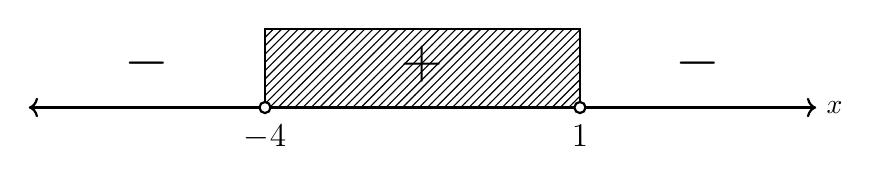
\begin{tikzpicture}
    \draw[thick,<->] (-5,0) -- (5,0) node[right] {$x$};
    \fill[pattern=north east lines] (-2,0) rectangle (2,1);
    \draw[thick] (-2,0) -- (-2,1) -- (2,1) -- (2,0);
    \draw (-2,-0.1) node[below] {\large{$-4$}};
    \draw (2,-0.1) node[below] {\large{$1$}};
    \draw (-3.5,0.2) node[above] {\huge{$-$}};
    \draw (0,0.2) node[above] {\huge{$+$}};
    \draw (3.5,0.2) node[above] {\huge{$-$}};
    \draw[fill=white, thick] (-2,0) circle (2pt);
    \draw[fill=white, thick] (2,0) circle (2pt);
            \end{tikzpicture}
        \end{center}
        Pembuat nol penyebut tidak diikutkan karena membuat ekspresi tidak terdefinisi. Jadi penyelesaiannya adalah $-4<x<1$, atau dalam notasi interval $\colorlet{oldcolor}{.}
        \color{red}
        \setlength{\fboxrule}{1pt} \boxed{\color{oldcolor}(-4,1)}\color{oldcolor}$.
    }
    \end{jawab}

    \item \textbf{[Subbab 1.5]} Gunakan grafik dasar $y=x^2$ dan sifat pergeseran/translasi untuk menggambar parabola $y=x^2+4x+1$. Tandai titik puncak dan titik potongnya dengan sumbu-sumbu koordinat.
    \begin{jawab}[parabola, melengkapkan kuadrat, translasi grafik]{~\\
        Kurva dasar $y=x^2$ merupakan parabola yang terbuka ke atas dengan titik puncak $(0,0)$. Selanjutnya, bentuk $y=x^2+4x+1$ diubah dengan cara melengkapkan kuadrat, yaitu
        \begin{align*}
            y &= x^2+4x+1\\
            &= (x^2+4x+4)-4+1\\
            &= \colorlet{oldcolor}{.}
        \color{blue}
        \setlength{\fboxrule}{1pt} \boxed{\color{oldcolor}(x+2)^2-3}\color{oldcolor}.
        \end{align*}
        Ingat kembali bahwa mengganti $x$ dengan $x+2$ berarti menggeser grafik sejauh $2$ satuan ke kiri, dan menambahkan konstanta $-3$ pada $y$ berarti menggeser grafik sejauh $3$ satuan ke bawah. Dengan demikian, proses translasinya adalah sebagai berikut.
        \begin{enumerate}
            \item[(i)] Gambar kurva dasar $y=x^2$ dengan titik puncak $(0,0)$.
            \item[(ii)] Geser kurva $y=x^2$ sejauh $2$ satuan ke kiri, sehingga diperoleh kurva $y=(x+2)^2$ dengan titik puncak $(-2,0)$.
            \item[(iii)] Geser kurva $y=(x+2)^2$ sejauh $3$ satuan ke bawah, sehingga diperoleh kurva $y=(x+2)^2-3$ dengan titik puncak $\colorlet{oldcolor}{.}
        \color{blue}
        \setlength{\fboxrule}{1pt} \boxed{\color{oldcolor}(-2,-3)}\color{oldcolor}$.
        \end{enumerate}
        Titik potong dengan sumbu-$y$ ($x=0$) adalah $y=1$, yaitu titik $\colorlet{oldcolor}{.}
        \color{blue}
        \setlength{\fboxrule}{1pt} \boxed{\color{oldcolor}(0,1)}\color{oldcolor}$, sedangkan titik potong dengan sumbu-$x$ ($y=0$) diperoleh dari $(x+2)^2=3$, yaitu $x=-2\pm\sqrt{3}$, sehingga titiknya adalah $\colorlet{oldcolor}{.}
        \color{blue}
        \setlength{\fboxrule}{1pt} \boxed{\color{oldcolor}\left(-2-\sqrt{3},0\right)}\color{oldcolor}$ dan $\colorlet{oldcolor}{.}
        \color{blue}
        \setlength{\fboxrule}{1pt} \boxed{\color{oldcolor}\left(-2+\sqrt{3},0\right)}\color{oldcolor}$. Sketsa grafiknya adalah sebagai berikut.
        \begin{center}
            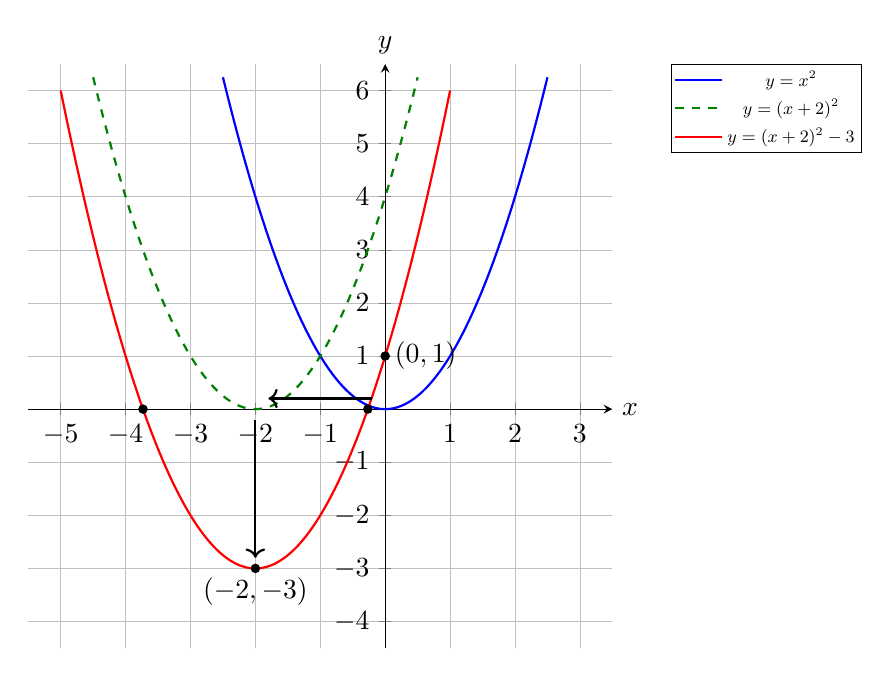
\begin{tikzpicture}
                \begin{axis}[
        axis lines = middle,
        xlabel = $x$,
        ylabel = {$y$},
        grid=both,
        grid style={line width=.1pt, draw=gray!10},
        major grid style={line width=.2pt,draw=gray!50},
        x label style={anchor=west}, % label x ke kanan
        y label style={anchor=south}, % label y ke atas
        samples=200,
        legend style={
                at={(1.1,1)},
                anchor=north west,
                font=\small,         % mengecilkan ukuran font
                row sep=1pt,         % jarak antar baris legend
                inner sep=1pt,       % margin dalam kotak legend
                nodes={scale=0.7}    % skalakan isi legend
            },
        xtick={-5,-4,...,3},
        ytick={-4,-3,...,6},
        xmin=-5.5, xmax=3.5,
        ymin=-4.5, ymax=6.5,
        width=9cm,
        height=9cm
    ]
\addplot[domain=-2.5:2.5, color=blue, thick] {x^2};
\addlegendentry{$y=x^2$}
\addplot[domain=-4.5:0.5, color=green!50!black, thick, dashed] {(x+2)^2};
\addlegendentry{$y=(x+2)^2$}
\addplot[domain=-5:1, color=red, thick] {(x+2)^2-3};
\addlegendentry{$y=(x+2)^2-3$}
\draw[fill=black] (-2,-3) circle (1.5pt) node[below] {$(-2,-3)$};
\draw[fill=black] (0,1) circle (1.5pt) node[right] {$(0,1)$};
\draw[fill=black] (-3.732,0) circle (1.5pt);
\draw[fill=black] (-0.268,0) circle (1.5pt);
\draw[->, thick] (-0.2,0.2) -- (-1.8,0.2);
\draw[->, thick] (-2,-0.2) -- (-2,-2.8);
\end{axis}
            \end{tikzpicture}
        \end{center}
        Jadi kurva $y=x^2+4x+1$ adalah
        \[\colorlet{oldcolor}{.}
        \color{red}
        \setlength{\fboxrule}{1pt} \boxed{\color{oldcolor}\text{parabola } y=x^2 \text{ yang digeser 2 satuan ke kiri dan 3 satuan ke bawah}}\color{oldcolor}.\]
    }
    \end{jawab}

    \item \textbf{[Subbab 2.4]} Diberikan fungsi sebagai berikut:
    \begin{align*}
        f(x)=\frac{2}{x-1};\quad \text{dan}\quad g(x)=\frac{x+2}{x}
    \end{align*}
    \begin{enumerate}
        \item Tentukan domain dan range dari masing-masing fungsi tersebut.
        \item Apakah kedua fungsi tersebut saling invers? Jelaskan alasannya.
    \end{enumerate}
    \begin{jawab}[domain dan range fungsi, fungsi rasional, fungsi invers, fungsi komposisi]{
        \begin{enumerate}
            \item Fungsi $f(x)=\frac{2}{x-1}$ terdefinisi untuk $x-1\neq 0$, sehingga $\colorlet{oldcolor}{.}
        \color{red}
        \setlength{\fboxrule}{1pt} \boxed{\color{oldcolor}D(f)=\mathbb{R}\setminus\{1\}}\color{oldcolor}$. Untuk menentukan range, misalkan $y=\frac{2}{x-1}$, maka
            \begin{align*}
                y(x-1) = 2 \iff x - 1 = \frac{2}{y} \iff x = 1+\frac{2}{y}.
            \end{align*}
            Nilai $x$ tersebut ada untuk setiap $y\neq 0$ (dan memang $\frac{2}{x-1}$ tidak pernah bernilai nol karena pembilangnya $2\neq 0$). Jadi $\colorlet{oldcolor}{.}
        \color{red}
        \setlength{\fboxrule}{1pt} \boxed{\color{oldcolor}R(f)=\mathbb{R}\setminus\{0\}}\color{oldcolor}$.\\
            Fungsi $g(x)=\frac{x+2}{x}$ terdefinisi untuk $x\neq 0$, sehingga $\colorlet{oldcolor}{.}
        \color{red}
        \setlength{\fboxrule}{1pt} \boxed{\color{oldcolor}D(g)=\mathbb{R}\setminus\{0\}}\color{oldcolor}$. Diperhatikan bahwa $g(x)=\frac{x+2}{x}=1+\frac{2}{x}$. Karena $\frac{2}{x}$ dapat bernilai sebarang bilangan real kecuali nol, maka $g(x)$ dapat bernilai sebarang bilangan real kecuali $1$. Jadi $\colorlet{oldcolor}{.}
        \color{red}
        \setlength{\fboxrule}{1pt} \boxed{\color{oldcolor}R(g)=\mathbb{R}\setminus\{1\}}\color{oldcolor}$.
            \item Dua fungsi $f$ dan $g$ saling invers jika
            \begin{align*}
                \colorlet{oldcolor}{.}
        \color{blue}
        \setlength{\fboxrule}{1pt} \boxed{\color{oldcolor}(f\circ g)(x)=x,~\forall x\in D(g)}\color{oldcolor} \quad\text{dan}\quad \colorlet{oldcolor}{.}
        \color{blue}
        \setlength{\fboxrule}{1pt} \boxed{\color{oldcolor}(g\circ f)(x)=x,~\forall x\in D(f)}\color{oldcolor}.
            \end{align*}
            Diperhatikan bahwa untuk $x\neq 0$,
            \begin{align*}
                (f\circ g)(x) = f\left(\frac{x+2}{x}\right) = \frac{2}{\frac{x+2}{x}-1} = \frac{2}{\frac{x+2-x}{x}} = \frac{2}{\frac{2}{x}} = x,
            \end{align*}
            dan untuk $x\neq 1$,
            \begin{align*}
                (g\circ f)(x) = g\left(\frac{2}{x-1}\right) = \frac{\frac{2}{x-1}+2}{\frac{2}{x-1}} = \frac{\frac{2+2(x-1)}{x-1}}{\frac{2}{x-1}} = \frac{2x}{2} = x.
            \end{align*}
            Selain itu, dari (a) terlihat bahwa $D(f)=R(g)=\mathbb{R}\setminus\{1\}$ dan $R(f)=D(g)=\mathbb{R}\setminus\{0\}$. Jadi $\colorlet{oldcolor}{.}
        \color{red}
        \setlength{\fboxrule}{1pt} \boxed{\color{oldcolor}f \text{ dan } g \text{ saling invers}}\color{oldcolor}$, yaitu $g=f^{-1}$ dan $f=g^{-1}$.
        \end{enumerate}
    }
    \end{jawab}

    \item \textbf{[Subbab 3.1]} Dapatkan nilai $k$ sedemikian sehingga $\displaystyle\lim_{x\to 2}f(x)$ ada, dimana
    \begin{align*}
        f(x)=\begin{cases}
            kx^2-1, & x<2\\
            3x+k, & x\geq 2
        \end{cases}.
    \end{align*}
    \begin{jawab}[limit sepihak, fungsi sepotong-sepotong]{~\\
        Ingat kembali bahwa $\displaystyle\lim_{x\to a}f(x)$ ada jika dan hanya jika limit kiri dan limit kanannya ada dan bernilai sama, yaitu $\colorlet{oldcolor}{.}
        \color{blue}
        \setlength{\fboxrule}{1pt} \boxed{\color{oldcolor}\lim_{x \to a^-} f(x) = \lim_{x \to a^+} f(x)}\color{oldcolor}$. Untuk $x\to 2^-$ (yaitu $x<2$) digunakan rumus $kx^2-1$, dan untuk $x\to 2^+$ (yaitu $x>2$) digunakan rumus $3x+k$. Diperoleh
        \begin{align*}
            \lim_{x\to 2^-} f(x) = \lim_{x\to 2^-} (kx^2-1) = 4k-1 \quad\text{dan}\quad \lim_{x\to 2^+} f(x) = \lim_{x\to 2^+} (3x+k) = 6+k.
        \end{align*}
        Agar limitnya ada, haruslah
        \begin{align*}
            4k-1 = 6+k \implies 3k = 7 \implies k = \frac{7}{3}.
        \end{align*}
        Jadi nilai $k$ yang membuat $\displaystyle\lim_{x\to 2}f(x)$ ada adalah $\colorlet{oldcolor}{.}
        \color{red}
        \setlength{\fboxrule}{1pt} \boxed{\color{oldcolor}k=\frac{7}{3}}\color{oldcolor}$. Sebagai pengecekan, untuk $k=\frac{7}{3}$ kedua limit sepihak bernilai $4\left(\frac{7}{3}\right)-1=\frac{25}{3}$ dan $6+\frac{7}{3}=\frac{25}{3}$.
    }
    \end{jawab}

    \item \textbf{[Subbab 4.4]} Dapatkan $f'(x)$ untuk $x>\frac{1}{2}$, dimana $f(x)=\sqrt{\dfrac{(2x-1)^3}{x}}$.
    \begin{jawab}[turunan fungsi, aturan perkalian, aturan rantai]{~\\
        Karena $x>\frac{1}{2}$, maka $2x-1>0$ dan $x>0$, sehingga fungsi dapat ditulis dalam bentuk pangkat, yaitu
        \begin{align*}
            f(x) = \frac{(2x-1)^{3/2}}{x^{1/2}} = \colorlet{oldcolor}{.}
        \color{blue}
        \setlength{\fboxrule}{1pt} \boxed{\color{oldcolor}(2x-1)^{3/2}\cdot x^{-1/2}}\color{oldcolor}.
        \end{align*}
        Ingat kembali aturan perkalian, yaitu $\colorlet{oldcolor}{.}
        \color{blue}
        \setlength{\fboxrule}{1pt} \boxed{\color{oldcolor}(uv)'=u'v+uv'}\color{oldcolor}$. Misalkan $u=(2x-1)^{3/2}$ dan $v=x^{-1/2}$. Dengan aturan rantai diperoleh
        \begin{align*}
            \colorlet{oldcolor}{.}
        \color{blue}
        \setlength{\fboxrule}{1pt} \boxed{\color{oldcolor}u' = \frac{3}{2}(2x-1)^{1/2}\cdot 2 = 3(2x-1)^{1/2}}\color{oldcolor} \quad\text{dan}\quad \colorlet{oldcolor}{.}
        \color{blue}
        \setlength{\fboxrule}{1pt} \boxed{\color{oldcolor}v' = -\frac{1}{2}x^{-3/2}}\color{oldcolor}.
        \end{align*}
        Dengan demikian, diperoleh
        \begin{align*}
            f'(x) &= 3(2x-1)^{1/2}x^{-1/2} + (2x-1)^{3/2}\left(-\frac{1}{2}x^{-3/2}\right)\\
            &= (2x-1)^{1/2}x^{-3/2}\left[3x - \frac{1}{2}(2x-1)\right]\\
            &= (2x-1)^{1/2}x^{-3/2}\cdot\frac{6x-2x+1}{2}\\
            &= \colorlet{oldcolor}{.}
        \color{red}
        \setlength{\fboxrule}{1pt} \boxed{\color{oldcolor}\frac{(4x+1)\sqrt{2x-1}}{2x\sqrt{x}}}\color{oldcolor}.
        \end{align*}
    }
    \end{jawab}
\end{enumerate}

\newpage

%%%%%%%%%%%%%%%%%%%%%%%%%%%%%%%%%%%%%%%%%%%%%%%%%%%%%%%%%%%%%%%%%%%%%%%%%%%%%%
% Kal-iup-1
% Kisi-kisi hari Senin: subbab 1.1, 1.5, 2.3, 2.4, 3.1, 3.3, 4.2, 4.4
\kopsoaliup{Kal-iup-1}{61, 68}{Chemical, Environmental, Electrical Engineering}{Monday, Wednesday; 07.00-09.30}{1}
\begin{enumerate}
    \item \textbf{[Subbab 1.1]} Solve the following inequality.
    \begin{align*}
        \frac{x^2-2x-8}{x^2-4x+3}\geq 0.
    \end{align*}
    \begin{jawab}[pertidaksamaan rasional, faktorisasi, garis bilangan, notasi interval]{~\\
    Karena ruas kanan pertidaksamaan sudah bernilai nol, maka kita bisa langsung memfaktorkan pembilang dan penyebut di ruas kiri. Diperoleh
    \begin{align*}
        \frac{x^2-2x-8}{x^2-4x+3} = \frac{(x-4)(x+2)}{(x-1)(x-3)} \geq 0.
    \end{align*}
    Selanjutnya, kita tentukan pembuat nol dari faktor-faktor tersebut, yaitu
    \begin{align*}
        x-4 = 0 \quad &\vee\quad x+2 = 0 \quad \vee\quad x-1 = 0 \quad \vee\quad x-3 = 0\\
        \colorlet{oldcolor}{.}
        \color{blue}
        \setlength{\fboxrule}{1pt} \boxed{\color{oldcolor}x=4}\color{oldcolor} \quad &\vee\quad \colorlet{oldcolor}{.}
        \color{blue}
        \setlength{\fboxrule}{1pt} \boxed{\color{oldcolor}x=-2}\color{oldcolor} \quad \vee\quad \colorlet{oldcolor}{.}
        \color{blue}
        \setlength{\fboxrule}{1pt} \boxed{\color{oldcolor}x=1}\color{oldcolor} \quad \vee\quad \colorlet{oldcolor}{.}
        \color{blue}
        \setlength{\fboxrule}{1pt} \boxed{\color{oldcolor}x=3}\color{oldcolor}
    \end{align*}
    Selanjutnya, kita buat garis bilangan dan lakukan uji titik pada ekspresi \(\frac{(x-4)(x+2)}{(x-1)(x-3)}\) sebagai berikut
    \begin{itemize}
        \item Untuk \(x < -2\), misalkan \(x = -3\):
        \[
        \frac{(-3-4)(-3+2)}{(-3-1)(-3-3)} = \frac{(-7)(-1)}{(-4)(-6)} = \frac{7}{24} > 0
        \]
        \item Untuk \(-2 < x < 1\), misalkan \(x = 0\):
        \[
        \frac{(0-4)(0+2)}{(0-1)(0-3)} = \frac{(-4)(2)}{(-1)(-3)} = \frac{-8}{3} < 0
        \]
        \item Untuk \(1 < x < 3\), misalkan \(x = 2\):
        \[
        \frac{(2-4)(2+2)}{(2-1)(2-3)} = \frac{(-2)(4)}{(1)(-1)} = 8 > 0
        \]
        \item Untuk \(3 < x < 4\), misalkan \(x = 3.5\):
        \[
        \frac{(3.5-4)(3.5+2)}{(3.5-1)(3.5-3)} = \frac{(-0.5)(5.5)}{(2.5)(0.5)} = \frac{-2.75}{1.25} < 0
        \]
        \item Untuk \(x > 4\), misalkan \(x = 5\):
        \[
        \frac{(5-4)(5+2)}{(5-1)(5-3)} = \frac{(1)(7)}{(4)(2)} = \frac{7}{8} > 0
        \]
    \end{itemize}
    \begin{center}
        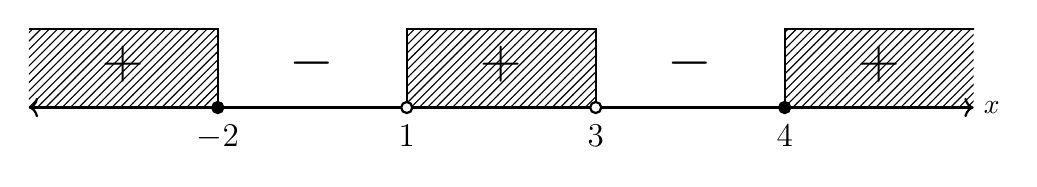
\begin{tikzpicture}
    \draw[thick,<->] (-6,0) -- (6,0) node[right] {$x$};
    \fill[pattern=north east lines] (-6,0) rectangle (-3.6,1);
    \fill[pattern=north east lines] (-1.2,0) rectangle (1.2,1);
    \fill[pattern=north east lines] (3.6,0) rectangle (6,1);
    \draw[thick] (-6,1) -- (-3.6,1) -- (-3.6,0);
    \draw[thick] (-1.2,0) -- (-1.2,1) -- (1.2,1) -- (1.2,0);
    \draw[thick] (3.6,0) -- (3.6,1) -- (6,1);
    \draw (-3.6,-0.1) node[below] {\large{$-2$}};
    \draw (-1.2,-0.1) node[below] {\large{$1$}};
    \draw (1.2,-0.1) node[below] {\large{$3$}};
    \draw (3.6,-0.1) node[below] {\large{$4$}};
    \draw (-4.8,0.2) node[above] {\huge{$+$}};
    \draw (-2.4,0.2) node[above] {\huge{$-$}};
    \draw (0,0.2) node[above] {\huge{$+$}};
    \draw (2.4,0.2) node[above] {\huge{$-$}};
    \draw (4.8,0.2) node[above] {\huge{$+$}};
    \draw[fill=black, thick] (-3.6,0) circle (2pt);
    \draw[fill=white, thick] (-1.2,0) circle (2pt);
    \draw[fill=white, thick] (1.2,0) circle (2pt);
    \draw[fill=black, thick] (3.6,0) circle (2pt);
        \end{tikzpicture}
    \end{center}
    Karena yang diminta adalah nilai yang lebih dari atau sama dengan nol, diambil interval yang bertanda positif beserta pembuat nol dari pembilang ($x=-2$ dan $x=4$). Pembuat nol dari penyebut ($x=1$ dan $x=3$) tidak diikutkan karena membuat ekspresi tidak terdefinisi. Jadi solusi dari pertidaksamaan tersebut adalah \(x \leq -2\) atau \(1 < x < 3\) atau \(x \geq 4\). Dalam notasi interval, solusi tersebut dapat ditulis sebagai $\colorlet{oldcolor}{.}
        \color{red}
        \setlength{\fboxrule}{1pt} \boxed{\color{oldcolor}(-\infty, -2] \cup (1, 3) \cup [4, \infty)}\color{oldcolor}$.
    }
    \end{jawab}

    \item \textbf{[Subbab 2.4]} Given a function $f(x)=2-\sqrt{x+4}$. Determine:
    \begin{enumerate}
        \item[a)] The domain and range of $f$;
        \item[b)] $f^{-1}(x)$ and its domain;
        \item[c)] Sketch the graph of $f(x)$ and $f^{-1}(x)$ in the same coordinate plane.
    \end{enumerate}
    \begin{jawab}[domain dan range fungsi, fungsi invers, sketsa grafik fungsi invers]{
        \begin{enumerate}
            \item Diperhatikan bahwa $f(x)$ memuat akar kuadrat, sehingga syaratnya adalah $x+4\geq 0$. Jadi $\colorlet{oldcolor}{.}
        \color{red}
        \setlength{\fboxrule}{1pt} \boxed{\color{oldcolor}D(f)=[-4,\infty)}\color{oldcolor}$. Selanjutnya, karena $\sqrt{x+4}\geq 0$ dan nilainya membesar tanpa batas, maka $2-\sqrt{x+4}\leq 2$ dan nilainya mengecil tanpa batas. Jadi $\colorlet{oldcolor}{.}
        \color{red}
        \setlength{\fboxrule}{1pt} \boxed{\color{oldcolor}R(f)=(-\infty,2]}\color{oldcolor}$.
            \item Untuk mendapatkan fungsi invers dari $f(x)$, kita misalkan $y=f(x)$, kemudian selesaikan sehingga terbentuk $x$ dalam fungsi $y$. Diperoleh
            \begin{align*}
                y &= 2-\sqrt{x+4}\\
                \sqrt{x+4} &= 2-y\\
                x+4 &= (2-y)^2\\
                x &= (2-y)^2-4.
            \end{align*}
            Dari sini didapatkan $x = f^{-1}(y) = (2-y)^2-4$. Dengan mengganti $y$ dengan $x$, diperoleh $f^{-1}(x)=(2-x)^2-4=x^2-4x$. Domain dari fungsi invers adalah range dari fungsi asli, yaitu $\colorlet{oldcolor}{.}
        \color{blue}
        \setlength{\fboxrule}{1pt} \boxed{\color{oldcolor}D(f^{-1})=R(f)=(-\infty,2]}\color{oldcolor}$, dan range dari fungsi invers adalah domain dari fungsi asli, yaitu $R(f^{-1})=D(f)=[-4,\infty)$. Jadi
            \begin{align*}
                \colorlet{oldcolor}{.}
        \color{red}
        \setlength{\fboxrule}{1pt} \boxed{\color{oldcolor}f^{-1}(x)=x^2-4x,\quad x\leq 2}\color{oldcolor}.
            \end{align*}
            Pembatasan $x\leq 2$ penting, karena tanpa pembatasan tersebut, fungsi $x^2-4x$ tidak satu-satu dan bukan invers dari $f$.
            \item Grafik $f$ adalah grafik $y=-\sqrt{x}$ yang digeser $4$ satuan ke kiri dan $2$ satuan ke atas, dimulai dari titik $(-4,2)$ dan melalui titik $(0,0)$ dan $(5,-1)$. Grafik $f^{-1}$ adalah pencerminan grafik $f$ terhadap garis $y=x$, yaitu bagian kiri parabola $y=(x-2)^2-4$ dengan ujung $(2,-4)$ dan melalui titik $(0,0)$ dan $(-1,5)$. Sketsa grafiknya adalah sebagai berikut.
            \begin{center}
                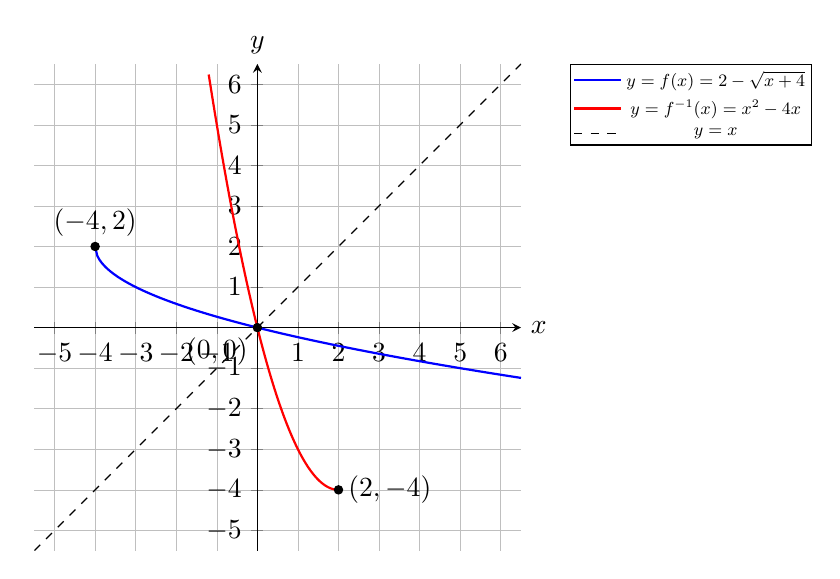
\begin{tikzpicture}
                    \begin{axis}[
        axis lines = middle,
        xlabel = $x$,
        ylabel = {$y$},
        grid=both,
        grid style={line width=.1pt, draw=gray!10},
        major grid style={line width=.2pt,draw=gray!50},
        x label style={anchor=west}, % label x ke kanan
        y label style={anchor=south}, % label y ke atas
        samples=200,
        legend style={
                at={(1.1,1)},
                anchor=north west,
                font=\small,         % mengecilkan ukuran font
                row sep=1pt,         % jarak antar baris legend
                inner sep=1pt,       % margin dalam kotak legend
                nodes={scale=0.7}    % skalakan isi legend
            },
        xtick={-5,-4,...,6},
        ytick={-5,-4,...,6},
        xmin=-5.5, xmax=6.5,
        ymin=-5.5, ymax=6.5,
        axis equal image,
        width=9cm
    ]
\addplot[domain=-4:6.5, color=blue, thick] {2-sqrt(x+4)};
\addlegendentry{$y=f(x)=2-\sqrt{x+4}$}
\addplot[domain=-1.2:2, color=red, thick] {x^2-4*x};
\addlegendentry{$y=f^{-1}(x)=x^2-4x$}
\addplot[domain=-5.5:6.5, color=black, dashed, samples=2] {x};
\addlegendentry{$y=x$}
\draw[fill=black] (-4,2) circle (1.5pt) node[above] {$(-4,2)$};
\draw[fill=black] (2,-4) circle (1.5pt) node[right] {$(2,-4)$};
\draw[fill=black] (0,0) circle (1.5pt) node[below left] {$(0,0)$};
\end{axis}
                \end{tikzpicture}
            \end{center}
        \end{enumerate}
    }
    \end{jawab}

    \item \textbf{[Subbab 4.4]} Write the chain rule formula for $\dfrac{d}{dx}\big[f(g(x))\big]$.\\
    Then, find the derivative of $h(x)=\sqrt{x^2+4x}$.
    \begin{jawab}[turunan, aturan rantai]{~\\
        Ingat kembali aturan rantai untuk turunan fungsi komposisi, yaitu
        \[
        \colorlet{oldcolor}{.}
        \color{red}
        \setlength{\fboxrule}{1pt} \boxed{\color{oldcolor}\frac{d}{dx}\big[f(g(x))\big] = f'(g(x)) \cdot g'(x)}\color{oldcolor}.
        \]
        Dapat dimisalkan $\colorlet{oldcolor}{.}
        \color{blue}
        \setlength{\fboxrule}{1pt} \boxed{\color{oldcolor}u=g(x)=x^2+4x}\color{oldcolor}$ sehingga $\colorlet{oldcolor}{.}
        \color{blue}
        \setlength{\fboxrule}{1pt} \boxed{\color{oldcolor}f(u)=\sqrt{u}=u^{1/2}}\color{oldcolor}$, dan diperoleh
        \begin{align*}
            \colorlet{oldcolor}{.}
        \color{blue}
        \setlength{\fboxrule}{1pt} \boxed{\color{oldcolor}f'(u)=\frac{1}{2}u^{-1/2}=\frac{1}{2\sqrt{u}}}\color{oldcolor} \quad\text{dan}\quad \colorlet{oldcolor}{.}
        \color{blue}
        \setlength{\fboxrule}{1pt} \boxed{\color{oldcolor}g'(x)=2x+4}\color{oldcolor}.
        \end{align*}
        Dengan demikian, diperoleh
        \begin{align*}
            h'(x) = \frac{1}{2\sqrt{x^2+4x}}\cdot(2x+4) = \colorlet{oldcolor}{.}
        \color{red}
        \setlength{\fboxrule}{1pt} \boxed{\color{oldcolor}\frac{x+2}{\sqrt{x^2+4x}}}\color{oldcolor}.
        \end{align*}
    }
    \end{jawab}

    \item \textbf{[Subbab 3.3]} Calculate $\displaystyle\lim_{x\to-\infty}\frac{\sqrt{4x^2+3}}{2-x}$.
    \begin{jawab}[limit di tak hingga, bentuk akar, nilai mutlak]{~\\
        Diperhatikan bahwa jika $x\to-\infty$, pembilang dan penyebut sama-sama menuju tak hingga, sehingga diperoleh bentuk tak tentu $\frac{\infty}{\infty}$. Untuk menyelesaikannya, keluarkan $x^2$ dari dalam akar dengan mengingat bahwa $\colorlet{oldcolor}{.}
        \color{blue}
        \setlength{\fboxrule}{1pt} \boxed{\color{oldcolor}\sqrt{x^2}=|x|}\color{oldcolor}$, dan karena $x\to-\infty$ (yaitu $x<0$), maka $\colorlet{oldcolor}{.}
        \color{blue}
        \setlength{\fboxrule}{1pt} \boxed{\color{oldcolor}|x|=-x}\color{oldcolor}$. Diperoleh
        \begin{align*}
            \sqrt{4x^2+3} = |x|\sqrt{4+\frac{3}{x^2}} = -x\sqrt{4+\frac{3}{x^2}}.
        \end{align*}
        Dengan demikian,
        \begin{align*}
            \lim_{x\to-\infty}\frac{\sqrt{4x^2+3}}{2-x} &= \lim_{x\to-\infty}\frac{-x\sqrt{4+\frac{3}{x^2}}}{-x\left(1-\frac{2}{x}\right)}\\
            &= \lim_{x\to-\infty}\frac{\sqrt{4+\frac{3}{x^2}}}{1-\frac{2}{x}}\\
            &= \frac{\sqrt{4+0}}{1-0}\\
            &= \colorlet{oldcolor}{.}
        \color{red}
        \setlength{\fboxrule}{1pt} \boxed{\color{oldcolor}2}\color{oldcolor}.
        \end{align*}
    }
    \end{jawab}

    \item \textbf{[Subbab 1.5]} Sketch the base curve $x=y^2$. Based on that base curve, use translation to sketch the curve $x=y^2-2y-3$. (Explain the process).
    \begin{jawab}[parabola, melengkapkan kuadrat, translasi grafik]{~\\
        Kurva dasar $x=y^2$ merupakan parabola yang terbuka ke kanan dengan titik puncak $(0,0)$. Selanjutnya, bentuk $x = y^2 - 2y - 3$ diubah dengan cara melengkapkan kuadrat, yaitu
        \begin{align*}
            x &= y^2 - 2y - 3\\
            &= (y^2 - 2y + 1) - 1 - 3\\
            &= \colorlet{oldcolor}{.}
        \color{blue}
        \setlength{\fboxrule}{1pt} \boxed{\color{oldcolor}(y-1)^2 - 4}\color{oldcolor}.
        \end{align*}
        Ingat kembali bahwa mengganti $y$ dengan $y-1$ berarti menggeser grafik sejauh $1$ satuan ke atas, dan menambahkan konstanta $-4$ pada $x$ berarti menggeser grafik sejauh $4$ satuan ke kiri. Dengan demikian, proses translasinya adalah sebagai berikut.
        \begin{enumerate}
            \item[(i)] Gambar kurva dasar $x=y^2$ dengan titik puncak $(0,0)$.
            \item[(ii)] Geser kurva $x=y^2$ sejauh $1$ satuan ke atas, sehingga diperoleh kurva $x=(y-1)^2$ dengan titik puncak $(0,1)$.
            \item[(iii)] Geser kurva $x=(y-1)^2$ sejauh $4$ satuan ke kiri, sehingga diperoleh kurva $x=(y-1)^2-4$ dengan titik puncak $\colorlet{oldcolor}{.}
        \color{blue}
        \setlength{\fboxrule}{1pt} \boxed{\color{oldcolor}(-4,1)}\color{oldcolor}$.
        \end{enumerate}
        Sebagai bantuan, titik potong kurva dengan sumbu-$x$ ($y=0$) adalah $x=-3$, yaitu titik $(-3,0)$, sedangkan titik potong dengan sumbu-$y$ ($x=0$) adalah $(y-1)^2=4$, yaitu $y=-1$ dan $y=3$. Sketsa grafiknya adalah sebagai berikut.
        \begin{center}
            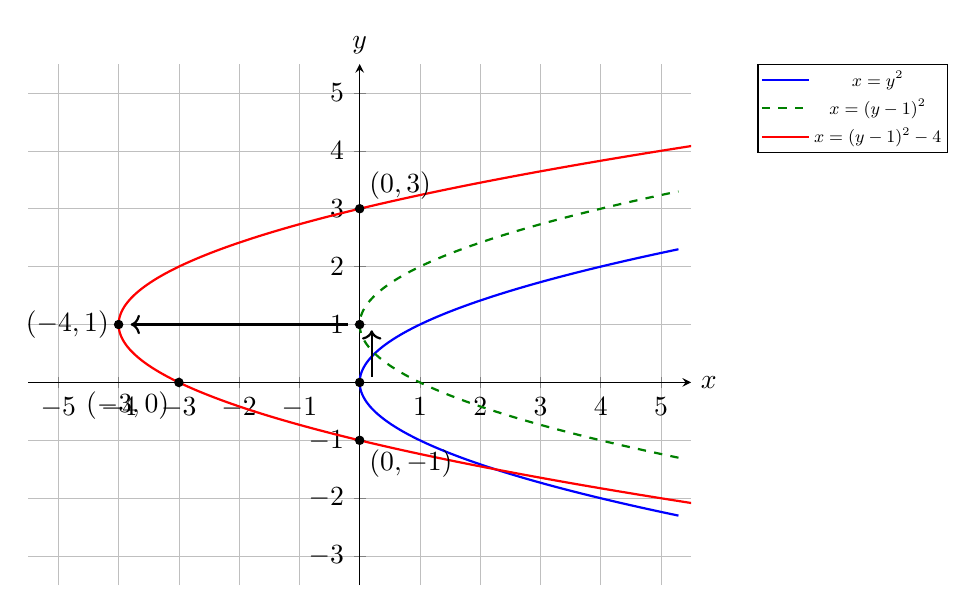
\begin{tikzpicture}
                \begin{axis}[
        axis lines = middle,
        xlabel = $x$,
        ylabel = {$y$},
        grid=both,
        grid style={line width=.1pt, draw=gray!10},
        major grid style={line width=.2pt,draw=gray!50},
        x label style={anchor=west}, % label x ke kanan
        y label style={anchor=south}, % label y ke atas
        samples=200,
        legend style={
                at={(1.1,1)},
                anchor=north west,
                font=\small,         % mengecilkan ukuran font
                row sep=1pt,         % jarak antar baris legend
                inner sep=1pt,       % margin dalam kotak legend
                nodes={scale=0.7}    % skalakan isi legend
            },
        xtick={-5,-4,...,5},
        ytick={-3,-2,...,5},
        xmin=-5.5, xmax=5.5,
        ymin=-3.5, ymax=5.5,
        width=10cm,
        height=8.2cm
    ]
\addplot[domain=-2.3:2.3, color=blue, thick] ({(x)*(x)},{x});
\addlegendentry{$x=y^2$}
\addplot[domain=-1.3:3.3, color=green!50!black, thick, dashed] ({(x-1)*(x-1)},{x});
\addlegendentry{$x=(y-1)^2$}
\addplot[domain=-2.2:4.2, color=red, thick] ({(x-1)*(x-1)-4},{x});
\addlegendentry{$x=(y-1)^2-4$}
\draw[fill=black] (0,0) circle (1.5pt);
\draw[fill=black] (0,1) circle (1.5pt);
\draw[fill=black] (-4,1) circle (1.5pt) node[left] {$(-4,1)$};
\draw[fill=black] (-3,0) circle (1.5pt) node[below left] {$(-3,0)$};
\draw[fill=black] (0,3) circle (1.5pt) node[above right] {$(0,3)$};
\draw[fill=black] (0,-1) circle (1.5pt) node[below right] {$(0,-1)$};
\draw[->, thick] (0.2,0.1) -- (0.2,0.9);
\draw[->, thick] (-0.2,1) -- (-3.8,1);
\end{axis}
            \end{tikzpicture}
        \end{center}
        Jadi kurva $x = y^2 - 2y - 3$ adalah
        \[\colorlet{oldcolor}{.}
        \color{red}
        \setlength{\fboxrule}{1pt} \boxed{\color{oldcolor}\text{parabola } x=y^2 \text{ yang digeser 1 satuan ke atas dan 4 satuan ke kiri}}\color{oldcolor}.\]
    }
    \end{jawab}
\end{enumerate}

\newpage

%%%%%%%%%%%%%%%%%%%%%%%%%%%%%%%%%%%%%%%%%%%%%%%%%%%%%%%%%%%%%%%%%%%%%%%%%%%%%%
% Kal-iup-4
% Kisi-kisi hari Senin: subbab 1.1, 1.5, 2.3, 2.4, 3.1, 3.3, 4.2, 4.4
\kopsoaliup{Kal-iup-4}{65, 66, 67}{Statistics, Marine Engineering (JD), Informatics}{Monday, Wednesday; 07.00-09.30}{1}
\begin{enumerate}
    \item \textbf{[Subbab 1.1]} Solve the following inequality.
    \begin{align*}
        \frac{x^2+2x-15}{x^2-x-2}\geq 0.
    \end{align*}
    \begin{jawab}[pertidaksamaan rasional, faktorisasi, garis bilangan, notasi interval]{~\\
    Karena ruas kanan pertidaksamaan sudah bernilai nol, maka kita bisa langsung memfaktorkan pembilang dan penyebut di ruas kiri. Diperoleh
    \begin{align*}
        \frac{x^2+2x-15}{x^2-x-2} = \frac{(x+5)(x-3)}{(x-2)(x+1)} \geq 0.
    \end{align*}
    Selanjutnya, kita tentukan pembuat nol dari faktor-faktor tersebut, yaitu
    \begin{align*}
        x+5 = 0 \quad &\vee\quad x-3 = 0 \quad \vee\quad x-2 = 0 \quad \vee\quad x+1 = 0\\
        \colorlet{oldcolor}{.}
        \color{blue}
        \setlength{\fboxrule}{1pt} \boxed{\color{oldcolor}x=-5}\color{oldcolor} \quad &\vee\quad \colorlet{oldcolor}{.}
        \color{blue}
        \setlength{\fboxrule}{1pt} \boxed{\color{oldcolor}x=3}\color{oldcolor} \quad \vee\quad \colorlet{oldcolor}{.}
        \color{blue}
        \setlength{\fboxrule}{1pt} \boxed{\color{oldcolor}x=2}\color{oldcolor} \quad \vee\quad \colorlet{oldcolor}{.}
        \color{blue}
        \setlength{\fboxrule}{1pt} \boxed{\color{oldcolor}x=-1}\color{oldcolor}
    \end{align*}
    Selanjutnya, kita buat garis bilangan dan lakukan uji titik pada ekspresi \(\frac{(x+5)(x-3)}{(x-2)(x+1)}\) sebagai berikut
    \begin{itemize}
        \item Untuk \(x < -5\), misalkan \(x = -6\):
        \[
        \frac{(-6+5)(-6-3)}{(-6-2)(-6+1)} = \frac{(-1)(-9)}{(-8)(-5)} = \frac{9}{40} > 0
        \]
        \item Untuk \(-5 < x < -1\), misalkan \(x = -2\):
        \[
        \frac{(-2+5)(-2-3)}{(-2-2)(-2+1)} = \frac{(3)(-5)}{(-4)(-1)} = \frac{-15}{4} < 0
        \]
        \item Untuk \(-1 < x < 2\), misalkan \(x = 0\):
        \[
        \frac{(0+5)(0-3)}{(0-2)(0+1)} = \frac{(5)(-3)}{(-2)(1)} = \frac{15}{2} > 0
        \]
        \item Untuk \(2 < x < 3\), misalkan \(x = 2.5\):
        \[
        \frac{(2.5+5)(2.5-3)}{(2.5-2)(2.5+1)} = \frac{(7.5)(-0.5)}{(0.5)(3.5)} = \frac{-3.75}{1.75} < 0
        \]
        \item Untuk \(x > 3\), misalkan \(x = 4\):
        \[
        \frac{(4+5)(4-3)}{(4-2)(4+1)} = \frac{(9)(1)}{(2)(5)} = \frac{9}{10} > 0
        \]
    \end{itemize}
    \begin{center}
        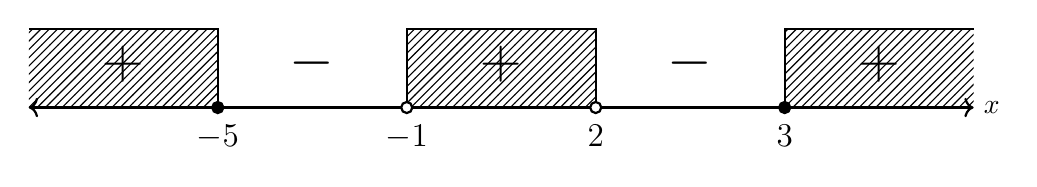
\begin{tikzpicture}
    \draw[thick,<->] (-6,0) -- (6,0) node[right] {$x$};
    \fill[pattern=north east lines] (-6,0) rectangle (-3.6,1);
    \fill[pattern=north east lines] (-1.2,0) rectangle (1.2,1);
    \fill[pattern=north east lines] (3.6,0) rectangle (6,1);
    \draw[thick] (-6,1) -- (-3.6,1) -- (-3.6,0);
    \draw[thick] (-1.2,0) -- (-1.2,1) -- (1.2,1) -- (1.2,0);
    \draw[thick] (3.6,0) -- (3.6,1) -- (6,1);
    \draw (-3.6,-0.1) node[below] {\large{$-5$}};
    \draw (-1.2,-0.1) node[below] {\large{$-1$}};
    \draw (1.2,-0.1) node[below] {\large{$2$}};
    \draw (3.6,-0.1) node[below] {\large{$3$}};
    \draw (-4.8,0.2) node[above] {\huge{$+$}};
    \draw (-2.4,0.2) node[above] {\huge{$-$}};
    \draw (0,0.2) node[above] {\huge{$+$}};
    \draw (2.4,0.2) node[above] {\huge{$-$}};
    \draw (4.8,0.2) node[above] {\huge{$+$}};
    \draw[fill=black, thick] (-3.6,0) circle (2pt);
    \draw[fill=white, thick] (-1.2,0) circle (2pt);
    \draw[fill=white, thick] (1.2,0) circle (2pt);
    \draw[fill=black, thick] (3.6,0) circle (2pt);
        \end{tikzpicture}
    \end{center}
    Karena yang diminta adalah nilai yang lebih dari atau sama dengan nol, diambil interval yang bertanda positif beserta pembuat nol dari pembilang ($x=-5$ dan $x=3$). Pembuat nol dari penyebut ($x=-1$ dan $x=2$) tidak diikutkan karena membuat ekspresi tidak terdefinisi. Jadi solusi dari pertidaksamaan tersebut adalah \(x \leq -5\) atau \(-1 < x < 2\) atau \(x \geq 3\). Dalam notasi interval, solusi tersebut dapat ditulis sebagai $\colorlet{oldcolor}{.}
        \color{red}
        \setlength{\fboxrule}{1pt} \boxed{\color{oldcolor}(-\infty, -5] \cup (-1, 2) \cup [3, \infty)}\color{oldcolor}$.
    }
    \end{jawab}

    \item \textbf{[Subbab 2.4]} Given a function $f(x)=3+\sqrt{x-1}$. Determine:
    \begin{enumerate}
        \item[a)] The domain and range of $f$;
        \item[b)] $f^{-1}(x)$ and its domain;
        \item[c)] Sketch the graph of $f(x)$ and $f^{-1}(x)$ in the same coordinate plane.
    \end{enumerate}
    \begin{jawab}[domain dan range fungsi, fungsi invers, sketsa grafik fungsi invers]{
        \begin{enumerate}
            \item Diperhatikan bahwa $f(x)$ memuat akar kuadrat, sehingga syaratnya adalah $x-1\geq 0$. Jadi $\colorlet{oldcolor}{.}
        \color{red}
        \setlength{\fboxrule}{1pt} \boxed{\color{oldcolor}D(f)=[1,\infty)}\color{oldcolor}$. Selanjutnya, karena $\sqrt{x-1}\geq 0$ dan nilainya membesar tanpa batas, maka $3+\sqrt{x-1}\geq 3$. Jadi $\colorlet{oldcolor}{.}
        \color{red}
        \setlength{\fboxrule}{1pt} \boxed{\color{oldcolor}R(f)=[3,\infty)}\color{oldcolor}$.
            \item Untuk mendapatkan fungsi invers dari $f(x)$, kita misalkan $y=f(x)$, kemudian selesaikan sehingga terbentuk $x$ dalam fungsi $y$. Diperoleh
            \begin{align*}
                y &= 3+\sqrt{x-1}\\
                \sqrt{x-1} &= y-3\\
                x-1 &= (y-3)^2\\
                x &= (y-3)^2+1.
            \end{align*}
            Dari sini didapatkan $x = f^{-1}(y) = (y-3)^2+1$. Dengan mengganti $y$ dengan $x$, diperoleh $f^{-1}(x)=(x-3)^2+1$. Domain dari fungsi invers adalah range dari fungsi asli, yaitu $\colorlet{oldcolor}{.}
        \color{blue}
        \setlength{\fboxrule}{1pt} \boxed{\color{oldcolor}D(f^{-1})=R(f)=[3,\infty)}\color{oldcolor}$, dan range dari fungsi invers adalah domain dari fungsi asli, yaitu $R(f^{-1})=D(f)=[1,\infty)$. Jadi
            \begin{align*}
                \colorlet{oldcolor}{.}
        \color{red}
        \setlength{\fboxrule}{1pt} \boxed{\color{oldcolor}f^{-1}(x)=(x-3)^2+1,\quad x\geq 3}\color{oldcolor}.
            \end{align*}
            \item Grafik $f$ adalah grafik $y=\sqrt{x}$ yang digeser $1$ satuan ke kanan dan $3$ satuan ke atas, dimulai dari titik $(1,3)$ dan melalui titik $(2,4)$ dan $(5,5)$. Grafik $f^{-1}$ adalah pencerminan grafik $f$ terhadap garis $y=x$, yaitu bagian kanan parabola $y=(x-3)^2+1$ dengan ujung $(3,1)$ dan melalui titik $(4,2)$ dan $(5,5)$. Sketsa grafiknya adalah sebagai berikut.
            \begin{center}
                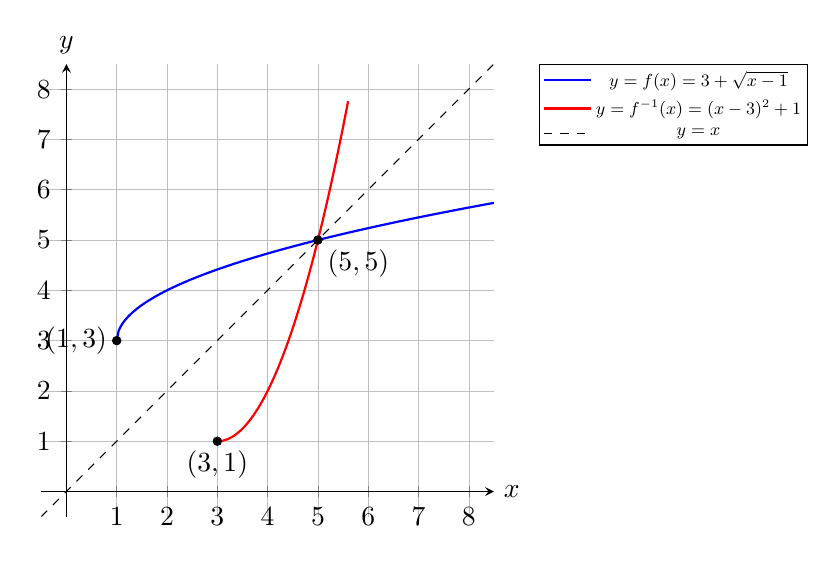
\begin{tikzpicture}
                    \begin{axis}[
        axis lines = middle,
        xlabel = $x$,
        ylabel = {$y$},
        grid=both,
        grid style={line width=.1pt, draw=gray!10},
        major grid style={line width=.2pt,draw=gray!50},
        x label style={anchor=west}, % label x ke kanan
        y label style={anchor=south}, % label y ke atas
        samples=200,
        legend style={
                at={(1.1,1)},
                anchor=north west,
                font=\small,         % mengecilkan ukuran font
                row sep=1pt,         % jarak antar baris legend
                inner sep=1pt,       % margin dalam kotak legend
                nodes={scale=0.7}    % skalakan isi legend
            },
        xtick={0,1,...,8},
        ytick={0,1,...,8},
        xmin=-0.5, xmax=8.5,
        ymin=-0.5, ymax=8.5,
        axis equal image,
        width=8.5cm
    ]
\addplot[domain=1:8.5, color=blue, thick] {3+sqrt(x-1)};
\addlegendentry{$y=f(x)=3+\sqrt{x-1}$}
\addplot[domain=3:5.6, color=red, thick] {(x-3)^2+1};
\addlegendentry{$y=f^{-1}(x)=(x-3)^2+1$}
\addplot[domain=-0.5:8.5, color=black, dashed, samples=2] {x};
\addlegendentry{$y=x$}
\draw[fill=black] (1,3) circle (1.5pt) node[left] {$(1,3)$};
\draw[fill=black] (3,1) circle (1.5pt) node[below] {$(3,1)$};
\draw[fill=black] (5,5) circle (1.5pt) node[below right] {$(5,5)$};
\end{axis}
                \end{tikzpicture}
            \end{center}
        \end{enumerate}
    }
    \end{jawab}

    \item \textbf{[Subbab 4.4]} Write the chain rule formula for $\dfrac{d}{dx}\big[f(g(x))\big]$.\\
    Then, find the derivative of $h(x)=\left(3x^2-2x\right)^4$.
    \begin{jawab}[turunan, aturan rantai]{~\\
        Ingat kembali aturan rantai untuk turunan fungsi komposisi, yaitu
        \[
        \colorlet{oldcolor}{.}
        \color{red}
        \setlength{\fboxrule}{1pt} \boxed{\color{oldcolor}\frac{d}{dx}\big[f(g(x))\big] = f'(g(x)) \cdot g'(x)}\color{oldcolor}.
        \]
        Dapat dimisalkan $\colorlet{oldcolor}{.}
        \color{blue}
        \setlength{\fboxrule}{1pt} \boxed{\color{oldcolor}u=g(x)=3x^2-2x}\color{oldcolor}$ sehingga $\colorlet{oldcolor}{.}
        \color{blue}
        \setlength{\fboxrule}{1pt} \boxed{\color{oldcolor}f(u)=u^4}\color{oldcolor}$, dan diperoleh
        \begin{align*}
            \colorlet{oldcolor}{.}
        \color{blue}
        \setlength{\fboxrule}{1pt} \boxed{\color{oldcolor}f'(u)=4u^3}\color{oldcolor} \quad\text{dan}\quad \colorlet{oldcolor}{.}
        \color{blue}
        \setlength{\fboxrule}{1pt} \boxed{\color{oldcolor}g'(x)=6x-2}\color{oldcolor}.
        \end{align*}
        Dengan demikian, diperoleh
        \begin{align*}
            h'(x) = 4\left(3x^2-2x\right)^3(6x-2) = \colorlet{oldcolor}{.}
        \color{red}
        \setlength{\fboxrule}{1pt} \boxed{\color{oldcolor}8(3x-1)\left(3x^2-2x\right)^3}\color{oldcolor}.
        \end{align*}
    }
    \end{jawab}

    \item \textbf{[Subbab 3.3]} Calculate $\displaystyle\lim_{x\to-\infty}\frac{\sqrt{4x^2+x}}{3x-1}$.
    \begin{jawab}[limit di tak hingga, bentuk akar, nilai mutlak]{~\\
        Diperhatikan bahwa jika $x\to-\infty$, diperoleh bentuk tak tentu $\frac{\infty}{-\infty}$. Keluarkan $x^2$ dari dalam akar dengan mengingat bahwa $\colorlet{oldcolor}{.}
        \color{blue}
        \setlength{\fboxrule}{1pt} \boxed{\color{oldcolor}\sqrt{x^2}=|x|}\color{oldcolor}$, dan karena $x\to-\infty$ (yaitu $x<0$), maka $\colorlet{oldcolor}{.}
        \color{blue}
        \setlength{\fboxrule}{1pt} \boxed{\color{oldcolor}|x|=-x}\color{oldcolor}$. Diperoleh
        \begin{align*}
            \lim_{x\to-\infty}\frac{\sqrt{4x^2+x}}{3x-1} &= \lim_{x\to-\infty}\frac{-x\sqrt{4+\frac{1}{x}}}{x\left(3-\frac{1}{x}\right)}\\
            &= \lim_{x\to-\infty}\frac{-\sqrt{4+\frac{1}{x}}}{3-\frac{1}{x}}\\
            &= \frac{-\sqrt{4+0}}{3-0}\\
            &= \colorlet{oldcolor}{.}
        \color{red}
        \setlength{\fboxrule}{1pt} \boxed{\color{oldcolor}-\frac{2}{3}}\color{oldcolor}.
        \end{align*}
        Hasil negatif ini masuk akal, karena untuk $x$ negatif yang sangat besar, pembilangnya positif sedangkan penyebutnya negatif.
    }
    \end{jawab}

    \item \textbf{[Subbab 1.5]} Sketch the base curve $x=y^2$. Based on that base curve, use translation to sketch the curve $x=y^2+6y+5$. (Explain the process).
    \begin{jawab}[parabola, melengkapkan kuadrat, translasi grafik]{~\\
        Kurva dasar $x=y^2$ merupakan parabola yang terbuka ke kanan dengan titik puncak $(0,0)$. Selanjutnya, bentuk $x = y^2 + 6y + 5$ diubah dengan cara melengkapkan kuadrat, yaitu
        \begin{align*}
            x &= y^2 + 6y + 5\\
            &= (y^2 + 6y + 9) - 9 + 5\\
            &= \colorlet{oldcolor}{.}
        \color{blue}
        \setlength{\fboxrule}{1pt} \boxed{\color{oldcolor}(y+3)^2 - 4}\color{oldcolor}.
        \end{align*}
        Ingat kembali bahwa mengganti $y$ dengan $y+3$ berarti menggeser grafik sejauh $3$ satuan ke bawah, dan menambahkan konstanta $-4$ pada $x$ berarti menggeser grafik sejauh $4$ satuan ke kiri. Dengan demikian, proses translasinya adalah sebagai berikut.
        \begin{enumerate}
            \item[(i)] Gambar kurva dasar $x=y^2$ dengan titik puncak $(0,0)$.
            \item[(ii)] Geser kurva $x=y^2$ sejauh $3$ satuan ke bawah, sehingga diperoleh kurva $x=(y+3)^2$ dengan titik puncak $(0,-3)$.
            \item[(iii)] Geser kurva $x=(y+3)^2$ sejauh $4$ satuan ke kiri, sehingga diperoleh kurva $x=(y+3)^2-4$ dengan titik puncak $\colorlet{oldcolor}{.}
        \color{blue}
        \setlength{\fboxrule}{1pt} \boxed{\color{oldcolor}(-4,-3)}\color{oldcolor}$.
        \end{enumerate}
        Sebagai bantuan, titik potong kurva dengan sumbu-$x$ ($y=0$) adalah $x=5$, yaitu titik $(5,0)$, sedangkan titik potong dengan sumbu-$y$ ($x=0$) adalah $(y+3)^2=4$, yaitu $y=-1$ dan $y=-5$. Sketsa grafiknya adalah sebagai berikut.
        \begin{center}
            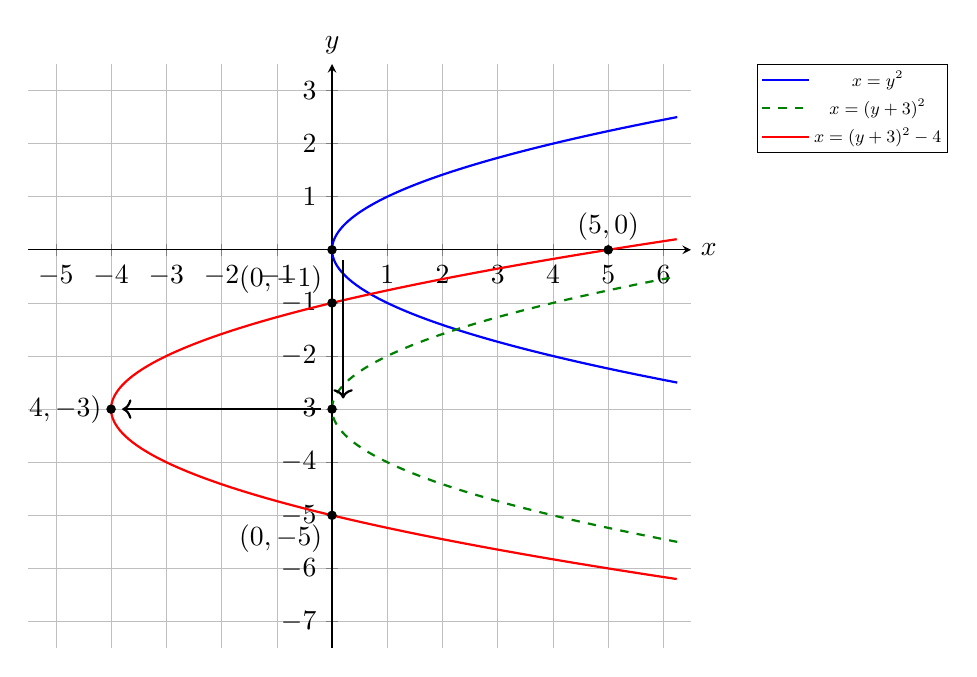
\begin{tikzpicture}
                \begin{axis}[
        axis lines = middle,
        xlabel = $x$,
        ylabel = {$y$},
        grid=both,
        grid style={line width=.1pt, draw=gray!10},
        major grid style={line width=.2pt,draw=gray!50},
        x label style={anchor=west}, % label x ke kanan
        y label style={anchor=south}, % label y ke atas
        samples=200,
        legend style={
                at={(1.1,1)},
                anchor=north west,
                font=\small,         % mengecilkan ukuran font
                row sep=1pt,         % jarak antar baris legend
                inner sep=1pt,       % margin dalam kotak legend
                nodes={scale=0.7}    % skalakan isi legend
            },
        xtick={-5,-4,...,6},
        ytick={-7,-6,...,3},
        xmin=-5.5, xmax=6.5,
        ymin=-7.5, ymax=3.5,
        width=10cm,
        height=9cm
    ]
\addplot[domain=-2.5:2.5, color=blue, thick] ({(x)*(x)},{x});
\addlegendentry{$x=y^2$}
\addplot[domain=-5.5:-0.5, color=green!50!black, thick, dashed] ({(x+3)*(x+3)},{x});
\addlegendentry{$x=(y+3)^2$}
\addplot[domain=-6.2:0.2, color=red, thick] ({(x+3)*(x+3)-4},{x});
\addlegendentry{$x=(y+3)^2-4$}
\draw[fill=black] (0,0) circle (1.5pt);
\draw[fill=black] (0,-3) circle (1.5pt);
\draw[fill=black] (-4,-3) circle (1.5pt) node[left] {$(-4,-3)$};
\draw[fill=black] (5,0) circle (1.5pt) node[above] {$(5,0)$};
\draw[fill=black] (0,-1) circle (1.5pt) node[above left] {$(0,-1)$};
\draw[fill=black] (0,-5) circle (1.5pt) node[below left] {$(0,-5)$};
\draw[->, thick] (0.2,-0.2) -- (0.2,-2.8);
\draw[->, thick] (-0.2,-3) -- (-3.8,-3);
\end{axis}
            \end{tikzpicture}
        \end{center}
        Jadi kurva $x = y^2 + 6y + 5$ adalah
        \[\colorlet{oldcolor}{.}
        \color{red}
        \setlength{\fboxrule}{1pt} \boxed{\color{oldcolor}\text{parabola } x=y^2 \text{ yang digeser 3 satuan ke bawah dan 4 satuan ke kiri}}\color{oldcolor}.\]
    }
    \end{jawab}
\end{enumerate}

\newpage

%%%%%%%%%%%%%%%%%%%%%%%%%%%%%%%%%%%%%%%%%%%%%%%%%%%%%%%%%%%%%%%%%%%%%%%%%%%%%%
% Kal-9
% Kisi-kisi hari Senin: subbab 1.1, 1.5, 2.3, 2.4, 3.1, 3.3, 4.2, 4.4
\kopsoal{Kal-9}{44-48}{T. Sistem Perkapalan, T. Kelautan, T. Komputer}{Senin, Rabu; 12.30-15.00}{3}
\begin{enumerate}
    \item \textbf{[Subbab 1.1]} Dapatkan himpunan penyelesaian dari $\dfrac{3}{x}\geq x+2$.
    \begin{jawab}[pertidaksamaan rasional, faktorisasi, garis bilangan, notasi interval]{~\\
        Untuk menyelesaikan pertidaksamaan rasional, pastikan ruas kanan sudah bernilai nol (jangan dikali dengan $x$, karena tanda $x$ belum diketahui). Diperoleh
        \begin{align*}
            \frac{3}{x}-(x+2) &\geq 0\\
            \frac{3-x^2-2x}{x} &\geq 0\\
            \frac{-(x^2+2x-3)}{x} &\geq 0\\
            \frac{(x+3)(x-1)}{x} &\leq 0.
        \end{align*}
        Diperhatikan bahwa ketika kedua ruas dikalikan $-1$, tanda pertidaksamaan berbalik. Pembuat nolnya adalah $\colorlet{oldcolor}{.}
        \color{blue}
        \setlength{\fboxrule}{1pt} \boxed{\color{oldcolor}x=-3}\color{oldcolor}$, $\colorlet{oldcolor}{.}
        \color{blue}
        \setlength{\fboxrule}{1pt} \boxed{\color{oldcolor}x=0}\color{oldcolor}$, dan $\colorlet{oldcolor}{.}
        \color{blue}
        \setlength{\fboxrule}{1pt} \boxed{\color{oldcolor}x=1}\color{oldcolor}$. Selanjutnya, dibuat garis bilangan dan dilakukan uji titik pada ekspresi $\frac{(x+3)(x-1)}{x}$ sebagai berikut
        \begin{itemize}
            \item Untuk \(x < -3\), misalkan \(x = -4\): $\displaystyle\frac{(-1)(-5)}{-4} = -\frac{5}{4} < 0$.
            \item Untuk \(-3 < x < 0\), misalkan \(x = -1\): $\displaystyle\frac{(2)(-2)}{-1} = 4 > 0$.
            \item Untuk \(0 < x < 1\), misalkan \(x = \frac{1}{2}\): $\displaystyle\frac{\left(\frac{7}{2}\right)\left(-\frac{1}{2}\right)}{\frac{1}{2}} = -\frac{7}{2} < 0$.
            \item Untuk \(x > 1\), misalkan \(x = 2\): $\displaystyle\frac{(5)(1)}{2} = \frac{5}{2} > 0$.
        \end{itemize}
        \begin{center}
           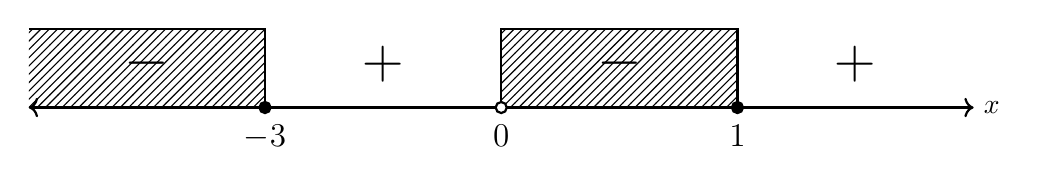
\begin{tikzpicture}
    \draw[thick,<->] (-6,0) -- (6,0) node[right] {$x$};
    \fill[pattern=north east lines] (-6,0) rectangle (-3,1);
    \fill[pattern=north east lines] (0,0) rectangle (3,1);
    \draw[thick] (-6,1) -- (-3,1) -- (-3,0);
    \draw[thick] (0,0) -- (0,1) -- (3,1) -- (3,0);
    \draw (-3,-0.1) node[below] {\large{$-3$}};
    \draw (0,-0.1) node[below] {\large{$0$}};
    \draw (3,-0.1) node[below] {\large{$1$}};
    \draw (-4.5,0.2) node[above] {\huge{$-$}};
    \draw (-1.5,0.2) node[above] {\huge{$+$}};
    \draw (1.5,0.2) node[above] {\huge{$-$}};
    \draw (4.5,0.2) node[above] {\huge{$+$}};
    \draw[fill=black, thick] (-3,0) circle (2pt);
    \draw[fill=white, thick] (0,0) circle (2pt);
    \draw[fill=black, thick] (3,0) circle (2pt);
\end{tikzpicture}
        \end{center}
        Karena yang diminta kurang dari atau sama dengan nol, diambil interval yang bertanda negatif beserta pembuat nol pembilang ($x=-3$ dan $x=1$), tetapi tanpa $x=0$ karena membuat ekspresi tidak terdefinisi. Jadi himpunan penyelesaiannya adalah
        \[
        \colorlet{oldcolor}{.}
        \color{red}
        \setlength{\fboxrule}{1pt} \boxed{\color{oldcolor}\{x\in\mathbb{R} : x\leq -3 \;\vee\; 0<x\leq 1\} = (-\infty,-3]\cup(0,1]}\color{oldcolor}.
        \]
    }
    \end{jawab}

    \item \textbf{[Subbab 1.5]} Diberikan lingkaran $x^2+y^2-6x+2y+1=0$.
    \begin{enumerate}
        \item Dapatkan pusat dan jari-jari lingkaran tersebut.
        \item Dapatkan persamaan setengah lingkaran bagian bawah dari lingkaran tersebut dalam bentuk $y=f(x)$, kemudian sketsa grafiknya.
    \end{enumerate}
    \begin{jawab}[persamaan lingkaran, melengkapkan kuadrat, setengah lingkaran, sketsa grafik]{
        \begin{enumerate}
            \item Persamaan lingkaran diubah ke bentuk baku dengan cara melengkapkan kuadrat, yaitu
            \begin{align*}
                x^2-6x+y^2+2y &= -1\\
                (x^2-6x+9)+(y^2+2y+1) &= -1+9+1\\
                (x-3)^2+(y+1)^2 &= 9.
            \end{align*}
            Jadi pusat dan jari-jari lingkaran adalah $\colorlet{oldcolor}{.}
        \color{red}
        \setlength{\fboxrule}{1pt} \boxed{\color{oldcolor}\text{Pusat: }(3,-1),~\text{Jari-jari: }3}\color{oldcolor}$.
            \item Dari bentuk baku, diperoleh
            \begin{align*}
                (y+1)^2 &= 9-(x-3)^2\\
                y+1 &= \pm\sqrt{9-(x-3)^2}\\
                y &= -1\pm\sqrt{9-(x-3)^2}.
            \end{align*}
            Tanda $+$ menghasilkan bagian atas lingkaran ($y\geq -1$), sedangkan tanda $-$ menghasilkan bagian bawah lingkaran ($y\leq -1$). Karena $9-(x-3)^2=9-x^2+6x-9=6x-x^2$, persamaan setengah lingkaran bagian bawah adalah
            \begin{align*}
                \colorlet{oldcolor}{.}
        \color{red}
        \setlength{\fboxrule}{1pt} \boxed{\color{oldcolor}y=-1-\sqrt{6x-x^2},\quad 0\leq x\leq 6}\color{oldcolor}.
            \end{align*}
            Grafiknya adalah setengah lingkaran bagian bawah dengan ujung-ujung $(0,-1)$ dan $(6,-1)$ serta titik terendah $(3,-4)$. Sketsa grafiknya adalah sebagai berikut:
            \begin{center}
                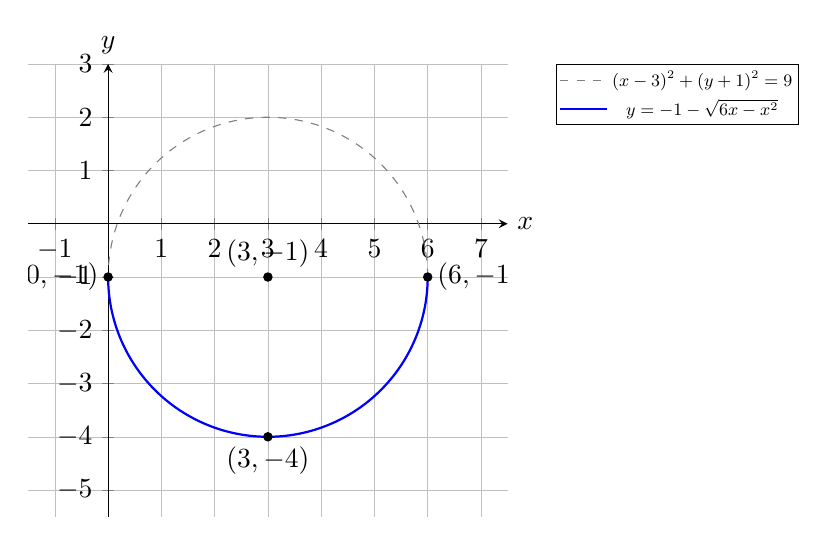
\begin{tikzpicture}
                    \begin{axis}[
        axis lines = middle,
        xlabel = $x$,
        ylabel = {$y$},
        grid=both,
        grid style={line width=.1pt, draw=gray!10},
        major grid style={line width=.2pt,draw=gray!50},
        x label style={anchor=west}, % label x ke kanan
        y label style={anchor=south}, % label y ke atas
        samples=200,
        legend style={
                at={(1.1,1)},
                anchor=north west,
                font=\small,         % mengecilkan ukuran font
                row sep=1pt,         % jarak antar baris legend
                inner sep=1pt,       % margin dalam kotak legend
                nodes={scale=0.7}    % skalakan isi legend
            },
        xtick={-1,0,...,7},
        ytick={-5,-4,...,3},
        xmin=-1.5, xmax=7.5,
        ymin=-5.5, ymax=3,
        axis equal image,
        width=8.5cm
    ]
\addplot[domain=0:360, color=gray, dashed] ({3+3*cos(x)}, {-1+3*sin(x)});
\addlegendentry{$(x-3)^2+(y+1)^2=9$}
\addplot[domain=180:360, color=blue, thick] ({3+3*cos(x)}, {-1+3*sin(x)});
\addlegendentry{$y=-1-\sqrt{6x-x^2}$}
\draw[fill=black] (3,-1) circle (1.5pt) node[above] {$(3,-1)$};
\draw[fill=black] (0,-1) circle (1.5pt) node[left] {$(0,-1)$};
\draw[fill=black] (6,-1) circle (1.5pt) node[right] {$(6,-1)$};
\draw[fill=black] (3,-4) circle (1.5pt) node[below] {$(3,-4)$};
\end{axis}
                \end{tikzpicture}
            \end{center}
        \end{enumerate}
    }
    \end{jawab}

    \item \textbf{[Subbab 2.4]} Diberikan $f(x)=\sqrt[3]{x+2},\ x\geq -2$.
    \begin{enumerate}
        \item Dapatkan $f^{-1}(x)$ beserta domainnya.
        \item Sketsa $f(x)$ dan $f^{-1}(x)$ pada satu bidang koordinat.
    \end{enumerate}
    \begin{jawab}[fungsi invers, domain dan range, sketsa grafik fungsi invers]{
        \begin{enumerate}
            \item Untuk mendapatkan fungsi invers dari $f(x)$, kita misalkan $y=f(x)$, kemudian selesaikan sehingga terbentuk $x$ dalam fungsi $y$. Diperoleh
            \begin{align*}
                y &= \sqrt[3]{x+2}\\
                y^3 &= x+2\\
                x &= y^3 - 2.
            \end{align*}
            Dari sini didapatkan $x = f^{-1}(y) = y^3 - 2$. Dengan mengganti $y$ dengan $x$, diperoleh $f^{-1}(x) = x^3 - 2$.\\
            Selanjutnya, karena domain $f$ dibatasi pada $x\geq -2$, maka $x+2\geq 0$ sehingga $\sqrt[3]{x+2}\geq 0$, dan nilainya membesar tanpa batas. Jadi range dari $f$ adalah $R(f)=[0,\infty)$. Domain dari fungsi invers adalah range dari fungsi asli, yaitu $\colorlet{oldcolor}{.}
        \color{blue}
        \setlength{\fboxrule}{1pt} \boxed{\color{oldcolor}D(f^{-1}) = R(f) = [0, \infty)}\color{oldcolor}$, serta range dari fungsi invers adalah domain dari fungsi asli, yaitu $\colorlet{oldcolor}{.}
        \color{blue}
        \setlength{\fboxrule}{1pt} \boxed{\color{oldcolor}R(f^{-1}) = D(f) = [-2, \infty)}\color{oldcolor}$. Jadi fungsi inversnya adalah
            \begin{align*}
                \colorlet{oldcolor}{.}
        \color{red}
        \setlength{\fboxrule}{1pt} \boxed{\color{oldcolor}f^{-1}(x) = x^3 - 2,\quad D(f^{-1})=[0,\infty)}\color{oldcolor}.
            \end{align*}
            \item Grafik $f^{-1}$ merupakan pencerminan grafik $f$ terhadap garis $y=x$. Sebagai bantuan, grafik $f$ melalui titik $(-2,0)$, $(-1,1)$, dan $(6,2)$, sehingga grafik $f^{-1}$ melalui titik $(0,-2)$, $(1,-1)$, dan $(2,6)$. Sketsa grafiknya adalah sebagai berikut.
            \begin{center}
                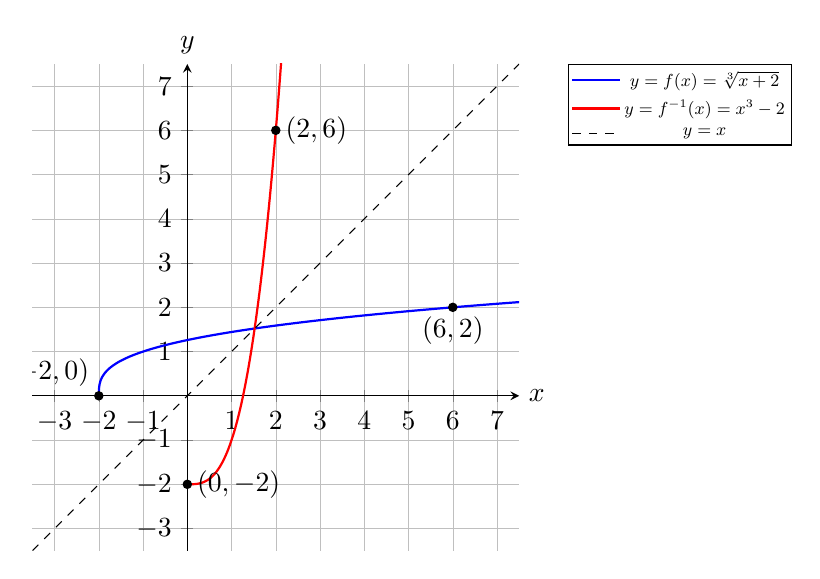
\begin{tikzpicture}
                    \begin{axis}[
        axis lines = middle,
        xlabel = $x$,
        ylabel = {$y$},
        grid=both,
        grid style={line width=.1pt, draw=gray!10},
        major grid style={line width=.2pt,draw=gray!50},
        x label style={anchor=west}, % label x ke kanan
        y label style={anchor=south}, % label y ke atas
        samples=200,
        legend style={
                at={(1.1,1)},
                anchor=north west,
                font=\small,         % mengecilkan ukuran font
                row sep=1pt,         % jarak antar baris legend
                inner sep=1pt,       % margin dalam kotak legend
                nodes={scale=0.7}    % skalakan isi legend
            },
        xtick={-3,-2,...,7},
        ytick={-3,-2,...,7},
        xmin=-3.5, xmax=7.5,
        ymin=-3.5, ymax=7.5,
        axis equal image,
        width=9cm
    ]
\addplot[domain=0:2.13, color=blue, thick, variable=\t] ({(\t)*(\t)*(\t)-2},{\t});
\addlegendentry{$y=f(x)=\sqrt[3]{x+2}$}
\addplot[domain=0:2.13, color=red, thick, variable=\t] ({\t},{(\t)*(\t)*(\t)-2});
\addlegendentry{$y=f^{-1}(x)=x^3-2$}
\addplot[domain=-3.5:7.5, color=black, dashed, samples=2] {x};
\addlegendentry{$y=x$}
\draw[fill=black] (-2,0) circle (1.5pt) node[above left] {$(-2,0)$};
\draw[fill=black] (6,2) circle (1.5pt) node[below] {$(6,2)$};
\draw[fill=black] (0,-2) circle (1.5pt) node[right] {$(0,-2)$};
\draw[fill=black] (2,6) circle (1.5pt) node[right] {$(2,6)$};
\end{axis}
                \end{tikzpicture}
            \end{center}
        \end{enumerate}
    }
    \end{jawab}

    \item \textbf{[Subbab 3.3]} Hitunglah $\displaystyle\lim_{y\to-\infty}\frac{3-2y}{\sqrt{5+9y^2}}$.
    \begin{jawab}[limit di tak hingga, bentuk akar, nilai mutlak]{~\\
        Diperhatikan bahwa jika $y\to-\infty$, pembilang dan penyebut sama-sama menuju tak hingga, sehingga diperoleh bentuk tak tentu $\frac{\infty}{\infty}$. Untuk menyelesaikannya, keluarkan $y^2$ dari dalam akar dengan mengingat bahwa $\colorlet{oldcolor}{.}
        \color{blue}
        \setlength{\fboxrule}{1pt} \boxed{\color{oldcolor}\sqrt{y^2}=|y|}\color{oldcolor}$, dan karena $y\to-\infty$ (yaitu $y<0$), maka $\colorlet{oldcolor}{.}
        \color{blue}
        \setlength{\fboxrule}{1pt} \boxed{\color{oldcolor}|y|=-y}\color{oldcolor}$. Diperoleh
        \begin{align*}
            \sqrt{5+9y^2} = \sqrt{y^2\left(\frac{5}{y^2}+9\right)} = |y|\sqrt{\frac{5}{y^2}+9} = -y\sqrt{\frac{5}{y^2}+9}.
        \end{align*}
        Dengan demikian,
        \begin{align*}
            \lim_{y\to-\infty}\frac{3-2y}{\sqrt{5+9y^2}} &= \lim_{y\to-\infty}\frac{3-2y}{-y\sqrt{\frac{5}{y^2}+9}}\\
            &= \lim_{y\to-\infty}\frac{-\frac{3}{y}+2}{\sqrt{\frac{5}{y^2}+9}}\\
            &= \frac{0+2}{\sqrt{0+9}}\\
            &= \colorlet{oldcolor}{.}
        \color{red}
        \setlength{\fboxrule}{1pt} \boxed{\color{oldcolor}\frac{2}{3}}\color{oldcolor}.
        \end{align*}
    }
    \end{jawab}

    \item \textbf{[Subbab 4.4]} Dapatkan persamaan garis singgung kurva $x^2+y+\dfrac{2y}{x}=\sqrt{x}+3$ di titik $(1,1)$.
    \begin{jawab}[diferensiasi implisit, aturan pembagian, persamaan garis singgung]{~\\
        Terlebih dahulu dicek bahwa titik $(1,1)$ terletak pada kurva, yaitu $1^2+1+\frac{2(1)}{1}=4$ dan $\sqrt{1}+3=4$. Selanjutnya, kita turunkan kedua ruas terhadap $x$, dengan mengingat bahwa $y$ adalah fungsi dari $x$. Dengan aturan pembagian, diperoleh
        \begin{align*}
            \colorlet{oldcolor}{.}
        \color{blue}
        \setlength{\fboxrule}{1pt} \boxed{\color{oldcolor}\frac{d}{dx}\left(\frac{2y}{x}\right) = \frac{2\frac{dy}{dx}\cdot x - 2y\cdot 1}{x^2} = \frac{2x\frac{dy}{dx} - 2y}{x^2}}\color{oldcolor}.
        \end{align*}
        Dengan demikian, diperoleh
        \begin{align*}
            2x + \frac{dy}{dx} + \frac{2x\frac{dy}{dx} - 2y}{x^2} = \frac{1}{2\sqrt{x}}.
        \end{align*}
        Selanjutnya, substitusi titik $(1,1)$ ke persamaan tersebut:
        \begin{align*}
            2(1) + \frac{dy}{dx} + \frac{2(1)\frac{dy}{dx} - 2(1)}{1^2} &= \frac{1}{2\sqrt{1}}\\
            2 + \frac{dy}{dx} + 2\frac{dy}{dx} - 2 &= \frac{1}{2}\\
            3\frac{dy}{dx} &= \frac{1}{2}\\
            \frac{dy}{dx}\bigg|_{(1,1)} &= \colorlet{oldcolor}{.}
        \color{blue}
        \setlength{\fboxrule}{1pt} \boxed{\color{oldcolor}\frac{1}{6}}\color{oldcolor}.
        \end{align*}
        Gradien garis singgung di titik $(1,1)$ adalah $m=\frac{1}{6}$. Dengan menggunakan persamaan garis $y - y_1 = m(x - x_1)$, di mana $(x_1,y_1)=(1,1)$, diperoleh
        \begin{align*}
            y - 1 &= \frac{1}{6}(x - 1)\\
            y &= \frac{1}{6}x + \frac{5}{6}.
        \end{align*}
        Jadi persamaan garis singgung di titik $(1,1)$ adalah $\colorlet{oldcolor}{.}
        \color{red}
        \setlength{\fboxrule}{1pt} \boxed{\color{oldcolor}y = \frac{1}{6}x + \frac{5}{6}}\color{oldcolor}$ atau $x-6y+5=0$.
    }
    \end{jawab}
\end{enumerate}

\newpage

%%%%%%%%%%%%%%%%%%%%%%%%%%%%%%%%%%%%%%%%%%%%%%%%%%%%%%%%%%%%%%%%%%%%%%%%%%%%%%
% Kal-11
% Kisi-kisi hari Senin: subbab 1.1, 1.5, 2.3, 2.4, 3.1, 3.3, 4.2, 4.4
\kopsoal{Kal-11}{51-54}{Biologi, Bioteknologi, Teknologi Informasi}{Senin, Rabu; 12.30-15.00}{3}
\begin{enumerate}
    \item \textbf{[Subbab 1.1]} Dapatkan penyelesaian dari pertidaksamaan
    \begin{align*}
        4\leq x^2+3x<10.
    \end{align*}
    \begin{jawab}[pertidaksamaan kuadrat, pertidaksamaan ganda, garis bilangan, notasi interval]{~\\
        Pertidaksamaan ganda tersebut dapat dipecah menjadi dua pertidaksamaan yang harus dipenuhi sekaligus, yaitu $\colorlet{oldcolor}{.}
        \color{blue}
        \setlength{\fboxrule}{1pt} \boxed{\color{oldcolor}x^2+3x\geq 4}\color{oldcolor}$ dan $\colorlet{oldcolor}{.}
        \color{blue}
        \setlength{\fboxrule}{1pt} \boxed{\color{oldcolor}x^2+3x<10}\color{oldcolor}$.
        \begin{itemize}
            \item Untuk $x^2+3x\geq 4$, diperoleh $x^2+3x-4=(x+4)(x-1)\geq 0$. Pembuat nolnya adalah $x=-4$ dan $x=1$. Dengan uji titik (misalnya $x=-5$, $x=0$, dan $x=2$), diperoleh tanda $+$, $-$, $+$, sehingga penyelesaiannya adalah $x\leq -4$ atau $x\geq 1$.
            \item Untuk $x^2+3x<10$, diperoleh $x^2+3x-10=(x+5)(x-2)<0$. Pembuat nolnya adalah $x=-5$ dan $x=2$. Dengan uji titik (misalnya $x=-6$, $x=0$, dan $x=3$), diperoleh tanda $+$, $-$, $+$, sehingga penyelesaiannya adalah $-5<x<2$.
        \end{itemize}
        Penyelesaian dari pertidaksamaan ganda adalah irisan dari kedua penyelesaian tersebut, yang dapat digambarkan pada garis bilangan sebagai berikut
        \begin{center}
            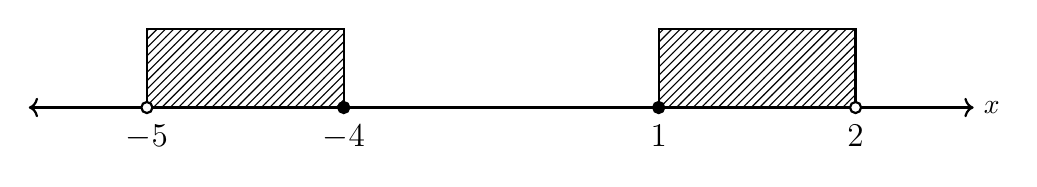
\begin{tikzpicture}
    \draw[thick,<->] (-6,0) -- (6,0) node[right] {$x$};
    \fill[pattern=north east lines] (-4.5,0) rectangle (-2,1);
    \fill[pattern=north east lines] (2,0) rectangle (4.5,1);
    \draw[thick] (-4.5,0) -- (-4.5,1) -- (-2,1) -- (-2,0);
    \draw[thick] (2,0) -- (2,1) -- (4.5,1) -- (4.5,0);
    \draw (-4.5,-0.1) node[below] {\large{$-5$}};
    \draw (-2,-0.1) node[below] {\large{$-4$}};
    \draw (2,-0.1) node[below] {\large{$1$}};
    \draw (4.5,-0.1) node[below] {\large{$2$}};
    \draw[fill=white, thick] (-4.5,0) circle (2pt);
    \draw[fill=black, thick] (-2,0) circle (2pt);
    \draw[fill=black, thick] (2,0) circle (2pt);
    \draw[fill=white, thick] (4.5,0) circle (2pt);
            \end{tikzpicture}
        \end{center}
        Sebagai pengecekan, untuk $x=\frac{3}{2}$ diperoleh $x^2+3x=\frac{27}{4}$ dan berlaku $4\leq\frac{27}{4}<10$. Jadi penyelesaiannya adalah $-5<x\leq -4$ atau $1\leq x<2$, atau dalam notasi interval $\colorlet{oldcolor}{.}
        \color{red}
        \setlength{\fboxrule}{1pt} \boxed{\color{oldcolor}(-5,-4]\cup[1,2)}\color{oldcolor}$.
    }
    \end{jawab}

    \item \textbf{[Subbab 1.5]} \begin{enumerate}
        \item Tentukan jarak titik $(-3,4)$ dan $(5,-2)$.
        \item Tentukan persamaan lingkaran yang diameternya adalah ruas garis dari titik $(-3,4)$ ke $(5,-2)$.
    \end{enumerate}
    \begin{jawab}[jarak titik, titik tengah, persamaan lingkaran]{
        \begin{enumerate}
            \item Ingat kembali rumus jarak antara dua titik $(x_1,y_1)$ dan $(x_2,y_2)$, yaitu
            \begin{align*}
                d = \sqrt{(x_2-x_1)^2+(y_2-y_1)^2}.
            \end{align*}
            Dengan substitusi $(x_1,y_1)=(-3,4)$ dan $(x_2,y_2)=(5,-2)$, diperoleh
            \begin{align*}
                d = \sqrt{(5-(-3))^2+(-2-4)^2}= \sqrt{8^2+(-6)^2}= \sqrt{64+36}= \sqrt{100}= 10.
            \end{align*}
            Jadi jarak antara titik $(-3,4)$ dan $(5,-2)$ adalah $\colorlet{oldcolor}{.}
        \color{red}
        \setlength{\fboxrule}{1pt} \boxed{\color{oldcolor}d = 10}\color{oldcolor}$.
            \item Diketahui bahwa diameter lingkaran adalah ruas garis dari titik $(-3,4)$ ke $(5,-2)$, sehingga jari-jari lingkaran adalah setengah dari panjang diameter, yaitu
            \begin{align*}
                \colorlet{oldcolor}{.}
        \color{blue}
        \setlength{\fboxrule}{1pt} \boxed{\color{oldcolor}r = \frac{d}{2} = \frac{10}{2} = 5}\color{oldcolor}.
            \end{align*}
            Karena kedua titik tersebut merupakan ujung-ujung diameter, maka pusat lingkaran adalah titik tengah dari dua titik tersebut. Titik tengah $(a,b)$ dari dua titik $(x_1,y_1)$ dan $(x_2,y_2)$ adalah
            \begin{align*}
                (a,b) = \left(\frac{x_1+x_2}{2},\frac{y_1+y_2}{2}\right).
            \end{align*}
            Dengan substitusi $(x_1,y_1)=(-3,4)$ dan $(x_2,y_2)=(5,-2)$, diperoleh
            \begin{align*}
                (a,b) = \left(\frac{-3+5}{2}, \frac{4+(-2)}{2}\right) = \left(\frac{2}{2}, \frac{2}{2}\right) = \colorlet{oldcolor}{.}
        \color{blue}
        \setlength{\fboxrule}{1pt} \boxed{\color{oldcolor}(1,1)}\color{oldcolor}.
            \end{align*}
            Persamaan lingkaran dengan pusat $(a,b)$ dan jari-jari $r$ adalah
            \begin{align*}
                (x-a)^2 + (y-b)^2 = r^2.
            \end{align*}
            Dengan substitusi $(a,b)=(1,1)$ dan $r=5$, diperoleh persamaan lingkarannya adalah
            $$\colorlet{oldcolor}{.}
        \color{red}
        \setlength{\fboxrule}{1pt} \boxed{\color{oldcolor}(x-1)^2 + (y-1)^2 = 25}\color{oldcolor}.$$
            atau dalam bentuk umum $x^2+y^2-2x-2y-23=0$.
        \end{enumerate}
    }
    \end{jawab}

    \item \textbf{[Subbab 2.4]} Diberikan fungsi $f(x)=x^2+2x-3$ dengan $x\leq -1$.
    \begin{enumerate}
        \item Dapatkan range dari $f(x)$.
        \item Dapatkan $f^{-1}(x)$ beserta domainnya.
        \item Sketsa grafik $f(x)$ dan $f^{-1}(x)$ pada satu bidang koordinat.
    \end{enumerate}
    \begin{jawab}[melengkapkan kuadrat, range fungsi, fungsi invers, sketsa grafik fungsi invers]{
        \begin{enumerate}
            \item Dengan melengkapkan kuadrat, diperoleh
            \begin{align*}
                f(x) = (x^2+2x+1)-1-3 = \colorlet{oldcolor}{.}
        \color{blue}
        \setlength{\fboxrule}{1pt} \boxed{\color{oldcolor}(x+1)^2-4}\color{oldcolor}.
            \end{align*}
            Grafik $f$ adalah parabola terbuka ke atas dengan titik puncak $(-1,-4)$. Karena domainnya dibatasi pada $x\leq -1$ (sebelah kiri titik puncak), fungsi $f$ turun dari $+\infty$ sampai $f(-1)=-4$. Jadi $\colorlet{oldcolor}{.}
        \color{red}
        \setlength{\fboxrule}{1pt} \boxed{\color{oldcolor}R(f)=[-4,\infty)}\color{oldcolor}$.
            \item Pada $x\leq -1$, fungsi $f$ satu-satu sehingga mempunyai invers. Misalkan $y=f(x)$, maka
            \begin{align*}
                y &= (x+1)^2-4\\
                (x+1)^2 &= y+4\\
                x+1 &= -\sqrt{y+4} \quad (\text{karena } x\leq -1, \text{ yaitu } x+1\leq 0)\\
                x &= -1-\sqrt{y+4}.
            \end{align*}
            Dengan mengganti $y$ dengan $x$, dan mengingat bahwa domain dari fungsi invers adalah range dari fungsi asli, diperoleh
            \begin{align*}
                \colorlet{oldcolor}{.}
        \color{red}
        \setlength{\fboxrule}{1pt} \boxed{\color{oldcolor}f^{-1}(x)=-1-\sqrt{x+4},\quad D(f^{-1})=[-4,\infty)}\color{oldcolor}.
            \end{align*}
            \item Grafik $f$ adalah bagian kiri parabola $y=(x+1)^2-4$, dimulai dari titik puncak $(-1,-4)$ dan melalui titik $(-3,0)$ dan $(-4,5)$. Grafik $f^{-1}$ adalah pencerminannya terhadap garis $y=x$, dimulai dari titik $(-4,-1)$ dan melalui titik $(0,-3)$ dan $(5,-4)$. Sketsa grafiknya adalah sebagai berikut.
            \begin{center}
                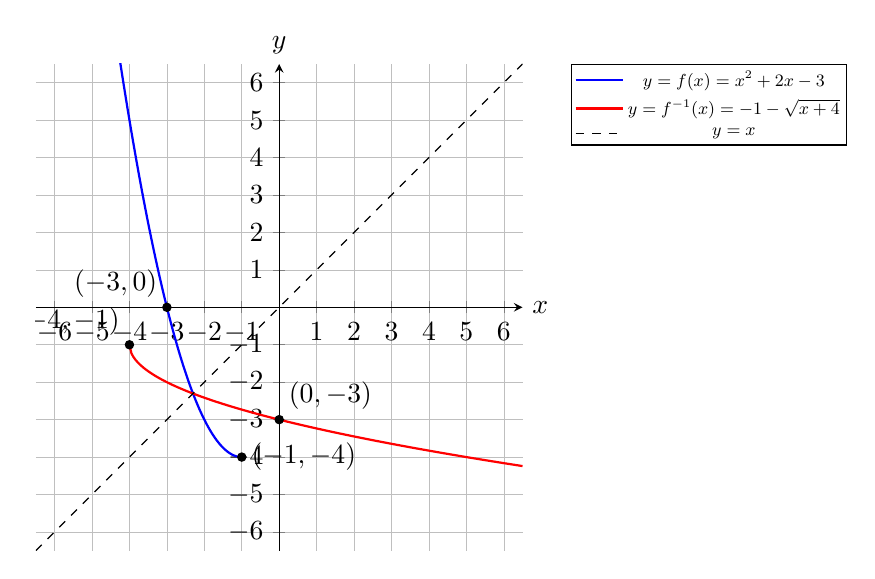
\begin{tikzpicture}
                    \begin{axis}[
        axis lines = middle,
        xlabel = $x$,
        ylabel = {$y$},
        grid=both,
        grid style={line width=.1pt, draw=gray!10},
        major grid style={line width=.2pt,draw=gray!50},
        x label style={anchor=west}, % label x ke kanan
        y label style={anchor=south}, % label y ke atas
        samples=200,
        legend style={
                at={(1.1,1)},
                anchor=north west,
                font=\small,         % mengecilkan ukuran font
                row sep=1pt,         % jarak antar baris legend
                inner sep=1pt,       % margin dalam kotak legend
                nodes={scale=0.7}    % skalakan isi legend
            },
        xtick={-6,-5,...,6},
        ytick={-6,-5,...,6},
        xmin=-6.5, xmax=6.5,
        ymin=-6.5, ymax=6.5,
        axis equal image,
        width=9cm
    ]
\addplot[domain=-4.6:-1, color=blue, thick] {(x+1)^2-4};
\addlegendentry{$y=f(x)=x^2+2x-3$}
\addplot[domain=-4:6.5, color=red, thick] {-1-sqrt(x+4)};
\addlegendentry{$y=f^{-1}(x)=-1-\sqrt{x+4}$}
\addplot[domain=-6.5:6.5, color=black, dashed, samples=2] {x};
\addlegendentry{$y=x$}
\draw[fill=black] (-1,-4) circle (1.5pt) node[right] {$(-1,-4)$};
\draw[fill=black] (-4,-1) circle (1.5pt) node[above left] {$(-4,-1)$};
\draw[fill=black] (-3,0) circle (1.5pt) node[above left] {$(-3,0)$};
\draw[fill=black] (0,-3) circle (1.5pt) node[above right] {$(0,-3)$};
\end{axis}
                \end{tikzpicture}
            \end{center}
        \end{enumerate}
    }
    \end{jawab}

    \item \textbf{[Subbab 3.1]} Diberikan $f(x)=\begin{cases}
        k^2(x+1), & x\leq 1\\
        (3-k)x, & x>1
    \end{cases}$.\\
    Tentukan semua nilai $k$ yang memenuhi agar $\displaystyle\lim_{x\to 1}f(x)$ ada.
    \begin{jawab}[limit sepihak, fungsi sepotong-sepotong, persamaan kuadrat]{~\\
        Ingat kembali bahwa $\displaystyle\lim_{x\to a}f(x)$ ada jika dan hanya jika limit kiri dan limit kanannya ada dan bernilai sama, yaitu $\colorlet{oldcolor}{.}
        \color{blue}
        \setlength{\fboxrule}{1pt} \boxed{\color{oldcolor}\lim_{x \to a^-} f(x) = \lim_{x \to a^+} f(x)}\color{oldcolor}$. Untuk $x\to 1^-$ (yaitu $x<1$) digunakan rumus $k^2(x+1)$, dan untuk $x\to 1^+$ (yaitu $x>1$) digunakan rumus $(3-k)x$. Diperoleh
        \begin{align*}
            \lim_{x\to 1^-} f(x) = \lim_{x\to 1^-} k^2(x+1) = 2k^2 \quad\text{dan}\quad \lim_{x\to 1^+} f(x) = \lim_{x\to 1^+} (3-k)x = 3-k.
        \end{align*}
        Agar limitnya ada, haruslah
        \begin{align*}
            2k^2 &= 3-k\\
            2k^2+k-3 &= 0\\
            (2k+3)(k-1) &= 0,
        \end{align*}
        sehingga $k=-\frac{3}{2}$ atau $k=1$. Jadi semua nilai $k$ yang memenuhi adalah $\colorlet{oldcolor}{.}
        \color{red}
        \setlength{\fboxrule}{1pt} \boxed{\color{oldcolor}k=-\frac{3}{2} \text{ atau } k=1}\color{oldcolor}$.\\
        Sebagai pengecekan, untuk $k=1$ kedua limit sepihak bernilai $2$, sedangkan untuk $k=-\frac{3}{2}$ kedua limit sepihak bernilai $\frac{9}{2}$.
    }
    \end{jawab}

    \item \textbf{[Subbab 4.4]} Diketahui kurva $x^3+xy-y^2=1$.
    \begin{enumerate}
        \item Dapatkan $\dfrac{dy}{dx}$ dengan menggunakan turunan fungsi implisit.
        \item Dari (a) dapatkan persamaan garis singgung pada kurva tersebut di titik $(1,1)$.
    \end{enumerate}
    \begin{jawab}[turunan implisit, aturan perkalian, persamaan garis singgung]{
        \begin{enumerate}
            \item Kita turunkan kedua ruas persamaan $x^3+xy-y^2=1$ terhadap $x$, dengan mengingat bahwa $y$ adalah fungsi dari $x$ (yaitu $y=y(x)$). Dengan aturan perkalian, $\colorlet{oldcolor}{.}
        \color{blue}
        \setlength{\fboxrule}{1pt} \boxed{\color{oldcolor}\frac{d}{dx}(xy) = y + x\frac{dy}{dx}}\color{oldcolor}$, dan dengan aturan rantai, $\colorlet{oldcolor}{.}
        \color{blue}
        \setlength{\fboxrule}{1pt} \boxed{\color{oldcolor}\frac{d}{dx}(y^2) = 2y\frac{dy}{dx}}\color{oldcolor}$. Diperoleh
            \begin{align*}
                \frac{d}{dx}(x^3) + \frac{d}{dx}(xy) - \frac{d}{dx}(y^2) &= \frac{d}{dx}(1)\\
                3x^2 + y + x\frac{dy}{dx} - 2y\frac{dy}{dx} &= 0.
            \end{align*}
            Selanjutnya, kumpulkan semua suku yang mengandung $\frac{dy}{dx}$ di satu ruas:
            \begin{align*}
                x\frac{dy}{dx} - 2y\frac{dy}{dx} &= -3x^2 - y\\
                (x - 2y)\frac{dy}{dx} &= -3x^2 - y\\
                \frac{dy}{dx} &= \frac{-3x^2 - y}{x - 2y} = \frac{3x^2+y}{2y-x}.
            \end{align*}
            Jadi diperoleh $\colorlet{oldcolor}{.}
        \color{red}
        \setlength{\fboxrule}{1pt} \boxed{\color{oldcolor}\frac{dy}{dx} = \frac{3x^2 + y}{2y - x}}\color{oldcolor}$.
            \item Terlebih dahulu dicek bahwa titik $(1,1)$ terletak pada kurva, yaitu $1^3+1(1)-1^2=1$. Untuk mendapatkan gradien garis singgung di titik $(1,1)$, substitusi $x=1$ dan $y=1$ ke dalam turunan yang telah diperoleh:
            \begin{align*}
                m=\left.\frac{dy}{dx}\right|_{(1,1)} = \frac{3(1)^2 + 1}{2(1) - 1}= \frac{4}{1}= \colorlet{oldcolor}{.}
        \color{blue}
        \setlength{\fboxrule}{1pt} \boxed{\color{oldcolor}4}\color{oldcolor}.
            \end{align*}
            Dengan menggunakan persamaan garis $y - y_1 = m(x - x_1)$, di mana $(x_1,y_1)=(1,1)$ dan $m=4$, diperoleh:
            \begin{align*}
                y - 1 &= 4(x - 1)\\
                y &= 4x - 3.
            \end{align*}
            Jadi persamaan garis singgung di titik $(1,1)$ adalah $\colorlet{oldcolor}{.}
        \color{red}
        \setlength{\fboxrule}{1pt} \boxed{\color{oldcolor}y = 4x - 3}\color{oldcolor}$ atau $4x-y=3$.
        \end{enumerate}
    }
    \end{jawab}
\end{enumerate}

\newpage

%%%%%%%%%%%%%%%%%%%%%%%%%%%%%%%%%%%%%%%%%%%%%%%%%%%%%%%%%%%%%%%%%%%%%%%%%%%%%%
% Kal-12
% Kisi-kisi hari Senin: subbab 1.1, 1.5, 2.3, 2.4, 3.1, 3.3, 4.2, 4.4
\kopsoal{Kal-12}{55-60}{Aktuaria, Teknik Informatika, RPL, RKA}{Senin, Rabu; 12.30-15.00}{3}
\begin{enumerate}
    \item \textbf{[Subbab 1.1]} Tentukan penyelesaian dari pertidaksamaan
    \begin{align*}
        \frac{2}{3-x}\geq\frac{3}{2x-1}.
    \end{align*}
    \begin{jawab}[pertidaksamaan rasional, pecahan, garis bilangan, notasi interval]{~\\
        Untuk menyelesaikan pertidaksamaan rasional, pastikan ruas kanan sudah bernilai nol (jangan dikali silang, karena tanda penyebutnya belum diketahui). Dengan mengurangkan \(\frac{3}{2x-1}\) dari kedua ruas dan menyamakan penyebut, diperoleh
        \begin{align}
            \frac{2(2x-1)-3(3-x)}{(3-x)(2x-1)} &\geq 0\nonumber\\
            \frac{4x-2-9+3x}{(3-x)(2x-1)} &\geq 0\nonumber\\
            \frac{7x-11}{(3-x)(2x-1)} &\geq 0 \label{ineq:kal12}
        \end{align}
        Didapatkan pembuat nol dari faktor-faktornya adalah
        \begin{align*}
            7x-11 = 0 \quad &\vee\quad  3-x = 0 \quad\vee\quad 2x-1=0\\
            \colorlet{oldcolor}{.}
        \color{blue}
        \setlength{\fboxrule}{1pt} \boxed{\color{oldcolor}x=\frac{11}{7}}\color{oldcolor} \quad &\vee\quad \colorlet{oldcolor}{.}
        \color{blue}
        \setlength{\fboxrule}{1pt} \boxed{\color{oldcolor}x=3}\color{oldcolor} \quad\vee\quad \colorlet{oldcolor}{.}
        \color{blue}
        \setlength{\fboxrule}{1pt} \boxed{\color{oldcolor}x=\frac{1}{2}}\color{oldcolor}
        \end{align*}
        Selanjutnya, dibuat garis bilangan dan dilakukan uji titik pada ekspresi \eqref{ineq:kal12} sebagai berikut
        \begin{itemize}
            \item Untuk \(x < \frac{1}{2}\), misalkan \(x = 0\): $\displaystyle\frac{-11}{(3)(-1)} = \frac{11}{3} > 0$.
            \item Untuk \(\frac{1}{2} < x < \frac{11}{7}\), misalkan \(x = 1\): $\displaystyle\frac{-4}{(2)(1)} = -2 < 0$.
            \item Untuk \(\frac{11}{7} < x < 3\), misalkan \(x = 2\): $\displaystyle\frac{3}{(1)(3)} = 1 > 0$.
            \item Untuk \(x > 3\), misalkan \(x = 4\): $\displaystyle\frac{17}{(-1)(7)} < 0$.
        \end{itemize}
        \begin{center}
           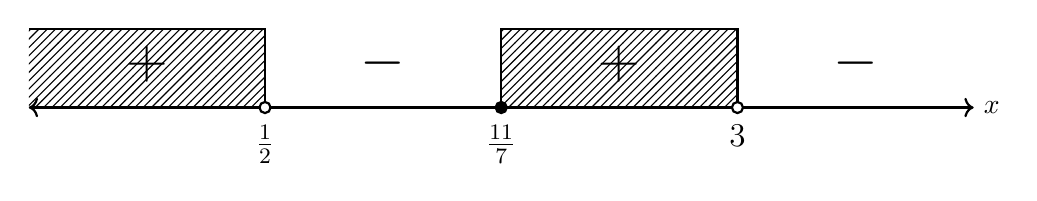
\begin{tikzpicture}
    \draw[thick,<->] (-6,0) -- (6,0) node[right] {$x$};
    \fill[pattern=north east lines] (-6,0) rectangle (-3,1);
    \fill[pattern=north east lines] (0,0) rectangle (3,1);
    \draw[thick] (-6,1) -- (-3,1) -- (-3,0);
    \draw[thick] (0,0) -- (0,1) -- (3,1) -- (3,0);
    \draw (-3,-0.1) node[below] {\large{$\frac{1}{2}$}};
    \draw (0,-0.1) node[below] {\large{$\frac{11}{7}$}};
    \draw (3,-0.1) node[below] {\large{$3$}};
    \draw (-4.5,0.2) node[above] {\huge{$+$}};
    \draw (-1.5,0.2) node[above] {\huge{$-$}};
    \draw (1.5,0.2) node[above] {\huge{$+$}};
    \draw (4.5,0.2) node[above] {\huge{$-$}};
    \draw[fill=white, thick] (-3,0) circle (2pt);
    \draw[fill=black, thick] (0,0) circle (2pt);
    \draw[fill=white, thick] (3,0) circle (2pt);
\end{tikzpicture}
        \end{center}
        Karena yang diminta lebih dari atau sama dengan nol, diambil interval yang bertanda positif beserta pembuat nol pembilang ($x=\frac{11}{7}$). Pembuat nol penyebut ($x=\frac{1}{2}$ dan $x=3$) tidak diikutkan karena membuat ekspresi tidak terdefinisi. Jadi penyelesaiannya adalah
        \[
        \colorlet{oldcolor}{.}
        \color{red}
        \setlength{\fboxrule}{1pt} \boxed{\color{oldcolor}\left(-\infty,\frac{1}{2}\right)\cup\left[\frac{11}{7},3\right)}\color{oldcolor}.
        \]
    }
    \end{jawab}

    \item \textbf{[Subbab 2.4]} Diberikan fungsi $f(x)=\sqrt{x+3}$.
    \begin{enumerate}
        \item Tentukan domain dan range dari fungsi $f(x)$.
        \item Tentukan $f^{-1}(x)$, domain dan range dari $f^{-1}(x)$.
    \end{enumerate}
    \begin{jawab}[domain dan range fungsi, fungsi invers]{
        \begin{enumerate}
            \item Diperhatikan bahwa $f(x)$ memuat akar kuadrat, sehingga domainnya adalah semua bilangan real yang membuat ekspresi di dalam akar kuadrat tak negatif. Jadi
            \begin{align*}
                \colorlet{oldcolor}{.}
        \color{red}
        \setlength{\fboxrule}{1pt} \boxed{\color{oldcolor}D(f)=\{x \in \mathbb{R} : x+3 \geq 0\} = [-3, \infty)}\color{oldcolor}.
            \end{align*}
            Selanjutnya, karena $f(x)$ merupakan fungsi akar kuadrat, maka nilainya selalu tak negatif, dan untuk $x$ yang membesar dari $-3$, nilai $\sqrt{x+3}$ membesar dari $0$ tanpa batas. Jadi
            \begin{align*}
                \colorlet{oldcolor}{.}
        \color{red}
        \setlength{\fboxrule}{1pt} \boxed{\color{oldcolor}R(f)=\{y \in \mathbb{R} : y \geq 0\} = [0, \infty)}\color{oldcolor}.
            \end{align*}
            \item Untuk mendapatkan fungsi invers dari $f(x)$, kita misalkan $y=f(x)$, kemudian selesaikan sehingga terbentuk $x$ dalam fungsi $y$. Diperoleh
            \begin{align*}
                y &= f(x) = \sqrt{x+3}\\
                y^2 &= x+3\\
                x &= y^2 - 3.
            \end{align*}
            Dari sini didapatkan $x = f^{-1}(y) = y^2 - 3$. Dengan mengganti $y$ dengan $x$, diperoleh
            \begin{align*}
                f^{-1}(x) = x^2 - 3.
            \end{align*}
            Selanjutnya, domain dari fungsi invers adalah range dari fungsi asli, yaitu $\colorlet{oldcolor}{.}
        \color{blue}
        \setlength{\fboxrule}{1pt} \boxed{\color{oldcolor}D(f^{-1}) = R(f) = [0, \infty)}\color{oldcolor}$, serta range dari fungsi invers adalah domain dari fungsi asli, yaitu $\colorlet{oldcolor}{.}
        \color{blue}
        \setlength{\fboxrule}{1pt} \boxed{\color{oldcolor}R(f^{-1}) = D(f) = [-3, \infty)}\color{oldcolor}$. Jadi fungsi inversnya adalah
        \begin{align*}
            \colorlet{oldcolor}{.}
        \color{red}
        \setlength{\fboxrule}{1pt} \boxed{\color{oldcolor}f^{-1}(x) = x^2 - 3,\quad x\geq 0}\color{oldcolor}.
        \end{align*}
        \end{enumerate}
    }
    \end{jawab}

    \item \textbf{[Subbab 1.5]} Diberikan persamaan separuh lingkaran
    \begin{align*}
        x=-2-\sqrt{-y^2+4y+12}.
    \end{align*}
    \begin{enumerate}
        \item Dapatkan pusat dan jari-jari lingkaran.
        \item Sketsa grafiknya.
    \end{enumerate}
    \begin{jawab}[persamaan lingkaran, pusat dan jari-jari lingkaran, sketsa grafik]{
        \begin{enumerate}
            \item Diperhatikan bahwa persamaan tersebut dapat ditulis ulang menjadi
            \begin{align*}
                x+2 &= -\sqrt{-y^2+4y+12}\\
                (x+2)^2 &= -y^2+4y+12\\
                (x+2)^2 + y^2 - 4y - 12 &= 0\\
                (x+2)^2 + (y^2 - 4y + 4) - 4 - 12 &= 0\\
                (x+2)^2 + (y-2)^2 &= 16.
            \end{align*}
            Dari persamaan tersebut, dapat dilihat bahwa pusat lingkaran adalah $(-2,2)$ dan jari-jari lingkaran adalah $\sqrt{16} = 4$. Jadi pusat dan jari-jari lingkaran adalah $\colorlet{oldcolor}{.}
        \color{red}
        \setlength{\fboxrule}{1pt} \boxed{\color{oldcolor}\text{Pusat: }(-2,2),~\text{Jari-jari: }4}\color{oldcolor}$.
            \item Diperhatikan bahwa pada persamaan $x=-2-\sqrt{-y^2+4y+12}$ berlaku $x+2=-\sqrt{-y^2+4y+12}\leq 0$, artinya $\colorlet{oldcolor}{.}
        \color{blue}
        \setlength{\fboxrule}{1pt} \boxed{\color{oldcolor}x\leq -2}\color{oldcolor}$. Sehingga grafik separuh lingkaran yang diberikan dalam soal merupakan bagian kiri dari lingkaran $(x+2)^2+(y-2)^2=16$, dengan ujung-ujung $(-2,-2)$ dan $(-2,6)$ serta titik paling kiri $(-6,2)$. Sketsa grafiknya adalah sebagai berikut:
            \begin{center}
                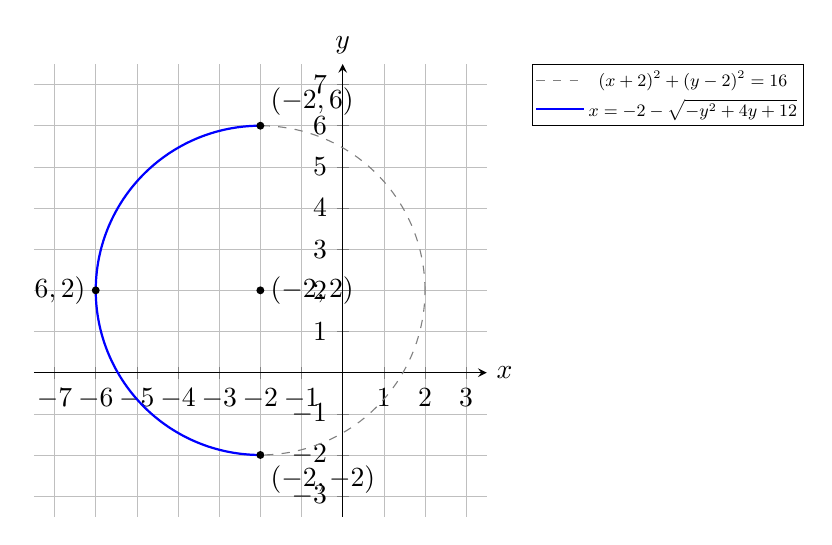
\begin{tikzpicture}
                   \begin{axis}[
        axis lines = middle,
        xlabel = $x$,
        ylabel = {$y$},
        grid=both,
        grid style={line width=.1pt, draw=gray!10},
        major grid style={line width=.2pt,draw=gray!50},
        x label style={anchor=west}, % label x ke kanan
        y label style={anchor=south}, % label y ke atas
        samples=200,
        legend style={
                at={(1.1,1)},
                anchor=north west,
                font=\small,         % mengecilkan ukuran font
                row sep=1pt,         % jarak antar baris legend
                inner sep=1pt,       % margin dalam kotak legend
                nodes={scale=0.7}    % skalakan isi legend
            },
        xtick={-7,-6,...,3},
        ytick={-3,-2,...,7},
        xmin=-7.5, xmax=3.5,
        ymin=-3.5, ymax=7.5,
        axis equal image,
        width=8.5cm
    ]
\addplot[domain=0:360, color=gray, dashed] ({-2+4*cos(x)}, {2+4*sin(x)});
\addlegendentry{$(x+2)^2+(y-2)^2=16$}
\addplot[domain=90:270, color=blue, thick] ({-2+4*cos(x)}, {2+4*sin(x)});
\addlegendentry{$x=-2-\sqrt{-y^2+4y+12}$}
\draw[fill=black, thick] (-2,2) circle (1pt) node[right] {$(-2,2)$};
\draw[fill=black, thick] (-2,-2) circle (1pt) node[below right] {$(-2,-2)$};
\draw[fill=black, thick] (-2,6) circle (1pt) node[above right] {$(-2,6)$};
\draw[fill=black, thick] (-6,2) circle (1pt) node[left] {$(-6,2)$};
\end{axis}
                \end{tikzpicture}
            \end{center}
            Grafik yang dimaksud adalah busur yang berwarna biru (setengah lingkaran bagian kiri).
        \end{enumerate}
    }
    \end{jawab}

    \item \textbf{[Subbab 3.3]} Hitunglah $\displaystyle\lim_{x\to+\infty}\left(2x-\sqrt{4x^2-3x}\right)$.
    \begin{jawab}[limit di tak hingga, bentuk tak tentu, perkalian sekawan]{~\\
        Jika $x\to+\infty$, diperoleh bentuk tak tentu $\infty-\infty$. Untuk menyelesaikannya, kita kalikan dengan bentuk sekawannya, sehingga diperoleh
        \begin{align*}
            \lim_{x\to+\infty}\left(2x-\sqrt{4x^2-3x}\right) &= \lim_{x\to+\infty}\left(2x-\sqrt{4x^2-3x}\right)\cdot\frac{2x+\sqrt{4x^2-3x}}{2x+\sqrt{4x^2-3x}}\\
            &= \lim_{x\to+\infty}\frac{4x^2-(4x^2-3x)}{2x+\sqrt{4x^2-3x}}\\
            &= \lim_{x\to+\infty}\frac{3x}{2x+\sqrt{4x^2-3x}}.
        \end{align*}
        Karena $x\to+\infty$ (yaitu $x>0$), maka $\colorlet{oldcolor}{.}
        \color{blue}
        \setlength{\fboxrule}{1pt} \boxed{\color{oldcolor}\sqrt{x^2}=|x|=x}\color{oldcolor}$. Dengan membagi pembilang dan penyebut dengan $x$, diperoleh
        \begin{align*}
            \lim_{x\to+\infty}\frac{3}{2+\sqrt{4-\frac{3}{x}}} = \frac{3}{2+\sqrt{4-0}} = \colorlet{oldcolor}{.}
        \color{red}
        \setlength{\fboxrule}{1pt} \boxed{\color{oldcolor}\frac{3}{4}}\color{oldcolor}.
        \end{align*}
    }
    \end{jawab}

    \item \textbf{[Subbab 4.4]} Diketahui fungsi $f(x)=\left(x^2-\dfrac{4}{x}\right)^{3/2}$. Dapatkan $f'(2)$.
    \begin{jawab}[turunan fungsi, aturan rantai]{~\\
        Ingat kembali aturan rantai untuk turunan fungsi, yaitu
        \[
        \colorlet{oldcolor}{.}
        \color{blue}
        \setlength{\fboxrule}{1pt} \boxed{\color{oldcolor}\frac{d}{dx}[h(g(x))] = h'(g(x)) \cdot g'(x)}\color{oldcolor}.
        \]
        Dapat dimisalkan $\colorlet{oldcolor}{.}
        \color{blue}
        \setlength{\fboxrule}{1pt} \boxed{\color{oldcolor}u=g(x) = x^2-\frac{4}{x}}\color{oldcolor}$ sehingga $\colorlet{oldcolor}{.}
        \color{blue}
        \setlength{\fboxrule}{1pt} \boxed{\color{oldcolor}h(u) = u^{3/2}}\color{oldcolor}$, dan diperoleh
        \begin{align*}
            \colorlet{oldcolor}{.}
        \color{blue}
        \setlength{\fboxrule}{1pt} \boxed{\color{oldcolor}h'(u) = \frac{3}{2}u^{1/2}}\color{oldcolor} \quad \text{dan}\quad
        \colorlet{oldcolor}{.}
        \color{blue}
        \setlength{\fboxrule}{1pt} \boxed{\color{oldcolor}g'(x) = 2x+\frac{4}{x^2}}\color{oldcolor}.
        \end{align*}
        Dengan demikian, diperoleh
        \begin{align*}
            f'(x) &=
            h'(u) \cdot g'(x)\\
            &= \frac{3}{2}u^{1/2} \cdot \left(2x+\frac{4}{x^2}\right)\\
            &= \colorlet{oldcolor}{.}
        \color{blue}
        \setlength{\fboxrule}{1pt} \boxed{\color{oldcolor}\frac{3}{2}\left(x^2-\frac{4}{x}\right)^{1/2} \left(2x+\frac{4}{x^2}\right)}\color{oldcolor}.
        \end{align*}
        Selanjutnya, substitusi $x=2$ ke dalam $f'(x)$, diperoleh
        \begin{align*}
            f'(2) &= \frac{3}{2}\left(4-\frac{4}{2}\right)^{1/2} \left(4+\frac{4}{4}\right)\\
            &= \frac{3}{2}\left(2\right)^{1/2} \left(5\right)\\
            &= \colorlet{oldcolor}{.}
        \color{red}
        \setlength{\fboxrule}{1pt} \boxed{\color{oldcolor}\frac{15}{2}\sqrt{2}}\color{oldcolor}.
        \end{align*}
    }
    \end{jawab}
\end{enumerate}

\newpage

%%%%%%%%%%%%%%%%%%%%%%%%%%%%%%%%%%%%%%%%%%%%%%%%%%%%%%%%%%%%%%%%%%%%%%%%%%%%%%
% Kal-7
% Kisi-kisi hari Senin: subbab 1.1, 1.5, 2.3, 2.4, 3.1, 3.3, 4.2, 4.4
\kopsoal{Kal-7}{32-37}{T. Sipil, T. Geomatika, T. Geofisika, T. Pertambangan}{Senin, Rabu; 15.30-17.10}{4}
\begin{enumerate}
    \item \textbf{[Subbab 1.1]} Dapatkan penyelesaian dari pertidaksamaan
    \begin{align*}
        \frac{4x-1}{x-2}\leq 3.
    \end{align*}
    \begin{jawab}[pertidaksamaan rasional, garis bilangan, notasi interval]{~\\
        Untuk menyelesaikan pertidaksamaan rasional, pastikan ruas kanan sudah bernilai nol (jangan dikali silang, karena tanda penyebutnya belum diketahui). Dengan mengurangkan $3$ dari kedua ruas, didapatkan
        \begin{align}
            \frac{4x-1}{x-2}-3 &\leq 0\nonumber\\
            \frac{4x-1-3(x-2)}{x-2} &\leq 0\nonumber\\
            \frac{x+5}{x-2} &\leq 0 \label{ineq:kal7}
        \end{align}
        Didapatkan pembuat nol dari faktor-faktornya adalah $\colorlet{oldcolor}{.}
        \color{blue}
        \setlength{\fboxrule}{1pt} \boxed{\color{oldcolor}x=-5}\color{oldcolor}$ dan $\colorlet{oldcolor}{.}
        \color{blue}
        \setlength{\fboxrule}{1pt} \boxed{\color{oldcolor}x=2}\color{oldcolor}$. Selanjutnya, dibuat garis bilangan dan dilakukan uji titik pada ekspresi \eqref{ineq:kal7} sebagai berikut
        \begin{itemize}
            \item Untuk \(x < -5\), misalkan \(x = -6\): $\displaystyle\frac{-1}{-8} > 0$.
            \item Untuk \(-5 < x < 2\), misalkan \(x = 0\): $\displaystyle\frac{5}{-2} < 0$.
            \item Untuk \(x > 2\), misalkan \(x = 3\): $\displaystyle\frac{8}{1} > 0$.
        \end{itemize}
        \begin{center}
           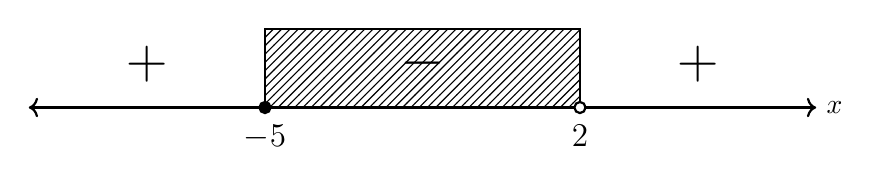
\begin{tikzpicture}
    \draw[thick,<->] (-5,0) -- (5,0) node[right] {$x$};
    \fill[pattern=north east lines] (-2,0) rectangle (2,1);
    \draw[thick] (-2,0) -- (-2,1) -- (2,1) -- (2,0);
    \draw (-2,-0.1) node[below] {\large{$-5$}};
    \draw (2,-0.1) node[below] {\large{$2$}};
    \draw (0,0.2) node[above] {\huge{$-$}};
    \draw (3.5,0.2) node[above] {\huge{$+$}};
    \draw (-3.5,0.2) node[above] {\huge{$+$}};
    \draw[fill=black, thick] (-2,0) circle (2pt);
    \draw[fill=white, thick] (2,0) circle (2pt);
\end{tikzpicture}
        \end{center}
        Karena yang diminta kurang dari atau sama dengan nol, diambil interval yang bertanda negatif beserta pembuat nol pembilang ($x=-5$), tetapi tanpa $x=2$ karena membuat ekspresi tidak terdefinisi. Jadi penyelesaiannya adalah $-5\leq x<2$, atau dalam notasi interval $\colorlet{oldcolor}{.}
        \color{red}
        \setlength{\fboxrule}{1pt} \boxed{\color{oldcolor}[-5,2)}\color{oldcolor}$.
    }
    \end{jawab}

    \item \textbf{[Subbab 1.5]} \begin{enumerate}
        \item Tentukan jarak titik $(-2,1)$ dan $(4,9)$.
        \item Tentukan persamaan lingkaran yang diameternya adalah ruas garis dari titik $(-2,1)$ ke $(4,9)$.
    \end{enumerate}
    \begin{jawab}[jarak titik, titik tengah, persamaan lingkaran]{
        \begin{enumerate}
            \item Ingat kembali rumus jarak antara dua titik $(x_1,y_1)$ dan $(x_2,y_2)$, yaitu
            \begin{align*}
                d = \sqrt{(x_2-x_1)^2+(y_2-y_1)^2}.
            \end{align*}
            Dengan substitusi $(x_1,y_1)=(-2,1)$ dan $(x_2,y_2)=(4,9)$, diperoleh
            \begin{align*}
                d = \sqrt{(4-(-2))^2+(9-1)^2}= \sqrt{6^2+8^2}= \sqrt{36+64}= \sqrt{100}= 10.
            \end{align*}
            Jadi jarak antara titik $(-2,1)$ dan $(4,9)$ adalah $\colorlet{oldcolor}{.}
        \color{red}
        \setlength{\fboxrule}{1pt} \boxed{\color{oldcolor}d = 10}\color{oldcolor}$.
            \item Diketahui bahwa diameter lingkaran adalah ruas garis dari titik $(-2,1)$ ke $(4,9)$, sehingga jari-jari lingkaran adalah setengah dari panjang diameter, yaitu
            \begin{align*}
                \colorlet{oldcolor}{.}
        \color{blue}
        \setlength{\fboxrule}{1pt} \boxed{\color{oldcolor}r = \frac{d}{2} = \frac{10}{2} = 5}\color{oldcolor}.
            \end{align*}
            Karena kedua titik tersebut merupakan ujung-ujung diameter, maka pusat lingkaran adalah titik tengah dari dua titik tersebut. Titik tengah $(a,b)$ dari dua titik $(x_1,y_1)$ dan $(x_2,y_2)$ adalah
            \begin{align*}
                (a,b) = \left(\frac{x_1+x_2}{2},\frac{y_1+y_2}{2}\right).
            \end{align*}
            Dengan substitusi $(x_1,y_1)=(-2,1)$ dan $(x_2,y_2)=(4,9)$, diperoleh
            \begin{align*}
                (a,b) = \left(\frac{-2+4}{2}, \frac{1+9}{2}\right) = \left(\frac{2}{2}, \frac{10}{2}\right) = \colorlet{oldcolor}{.}
        \color{blue}
        \setlength{\fboxrule}{1pt} \boxed{\color{oldcolor}(1,5)}\color{oldcolor}.
            \end{align*}
            Persamaan lingkaran dengan pusat $(a,b)$ dan jari-jari $r$ adalah
            \begin{align*}
                (x-a)^2 + (y-b)^2 = r^2.
            \end{align*}
            Dengan substitusi $(a,b)=(1,5)$ dan $r=5$, diperoleh persamaan lingkarannya adalah
            $$\colorlet{oldcolor}{.}
        \color{red}
        \setlength{\fboxrule}{1pt} \boxed{\color{oldcolor}(x-1)^2 + (y-5)^2 = 25}\color{oldcolor}.$$
            atau dalam bentuk umum $x^2+y^2-2x-10y+1=0$.
        \end{enumerate}
    }
    \end{jawab}

    \item \textbf{[Subbab 2.4]} Diberikan suatu fungsi $f(x)=3-\sqrt{9-x^2}$ dengan domain $f$ adalah $[a,3]$.
    \begin{enumerate}
        \item Tentukan nilai terkecil $a$ agar $f^{-1}(x)$ ada.
        \item Dapatkan $f^{-1}(x)$.
        \item Sketsa grafik $f(x)$ dan $f^{-1}(x)$ pada satu bidang koordinat.
    \end{enumerate}
    \begin{jawab}[fungsi satu-satu, setengah lingkaran, fungsi invers, sketsa grafik fungsi invers]{
        \begin{enumerate}
            \item Suatu fungsi mempunyai invers jika fungsi tersebut satu-satu (injektif). Diperhatikan bahwa jika $y=3-\sqrt{9-x^2}$, maka $3-y=\sqrt{9-x^2}\geq 0$ dan
            \begin{align*}
                (3-y)^2 = 9-x^2 \iff \colorlet{oldcolor}{.}
        \color{blue}
        \setlength{\fboxrule}{1pt} \boxed{\color{oldcolor}x^2+(y-3)^2=9}\color{oldcolor},\quad y\leq 3,
            \end{align*}
            sehingga grafik $f$ adalah setengah lingkaran bagian bawah dengan pusat $(0,3)$ dan jari-jari $3$. Grafik ini turun pada $[-3,0]$ dan naik pada $[0,3]$, sehingga jika domainnya memuat titik di kiri dan kanan $x=0$, fungsi $f$ tidak satu-satu (misalnya $f(-3)=f(3)=3$). Agar $f$ satu-satu pada $[a,3]$, haruslah $a\geq 0$. Jadi nilai terkecil $a$ adalah $\colorlet{oldcolor}{.}
        \color{red}
        \setlength{\fboxrule}{1pt} \boxed{\color{oldcolor}a=0}\color{oldcolor}$.
            \item Misalkan $y=f(x)$ dengan $x\in[0,3]$, kemudian selesaikan sehingga terbentuk $x$ dalam fungsi $y$. Diperoleh
            \begin{align*}
                y &= 3-\sqrt{9-x^2}\\
                \sqrt{9-x^2} &= 3-y\\
                9-x^2 &= (3-y)^2\\
                x^2 &= 9-(3-y)^2 = 6y-y^2\\
                x &= \sqrt{6y-y^2} \quad (\text{karena } x\geq 0).
            \end{align*}
            Dari sini didapatkan $x = f^{-1}(y) = \sqrt{6y-y^2}$. Dengan mengganti $y$ dengan $x$, diperoleh
            \begin{align*}
                \colorlet{oldcolor}{.}
        \color{red}
        \setlength{\fboxrule}{1pt} \boxed{\color{oldcolor}f^{-1}(x) = \sqrt{6x-x^2}}\color{oldcolor}.
            \end{align*}
            Pada domain $[0,3]$, fungsi $f$ naik dari $f(0)=0$ sampai $f(3)=3$, sehingga $R(f)=[0,3]$. Akibatnya, $D(f^{-1})=R(f)=[0,3]$ dan $R(f^{-1})=D(f)=[0,3]$.
            \item Grafik $f$ adalah seperempat lingkaran berpusat di $(0,3)$ dan berjari-jari $3$ dari titik $(0,0)$ ke $(3,3)$. Grafik $f^{-1}$ merupakan pencerminan grafik $f$ terhadap garis $y=x$, yaitu seperempat lingkaran $(x-3)^2+y^2=9$ yang berpusat di $(3,0)$, juga dari titik $(0,0)$ ke $(3,3)$. Sketsa grafiknya adalah sebagai berikut.
            \begin{center}
                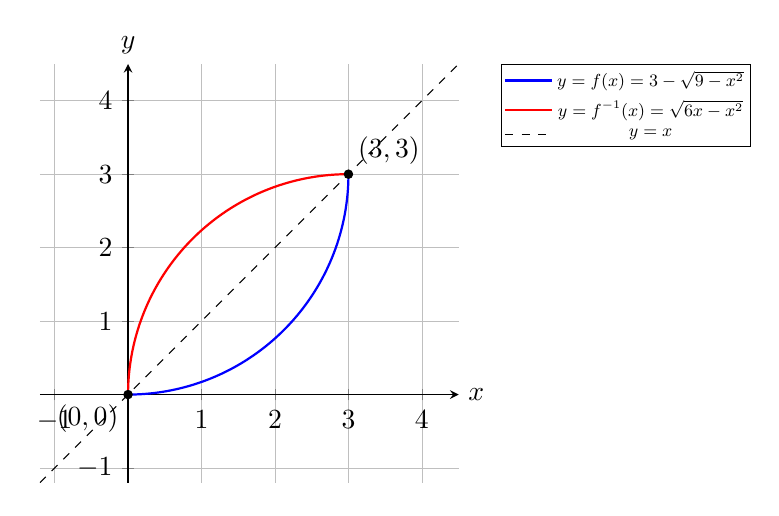
\begin{tikzpicture}
                    \begin{axis}[
        axis lines = middle,
        xlabel = $x$,
        ylabel = {$y$},
        grid=both,
        grid style={line width=.1pt, draw=gray!10},
        major grid style={line width=.2pt,draw=gray!50},
        x label style={anchor=west}, % label x ke kanan
        y label style={anchor=south}, % label y ke atas
        samples=200,
        legend style={
                at={(1.1,1)},
                anchor=north west,
                font=\small,         % mengecilkan ukuran font
                row sep=1pt,         % jarak antar baris legend
                inner sep=1pt,       % margin dalam kotak legend
                nodes={scale=0.7}    % skalakan isi legend
            },
        xtick={-1,0,...,4},
        ytick={-1,0,...,4},
        xmin=-1.2, xmax=4.5,
        ymin=-1.2, ymax=4.5,
        axis equal image,
        width=8cm
    ]
\addplot[domain=-90:0, color=blue, thick] ({3*cos(x)}, {3+3*sin(x)});
\addlegendentry{$y=f(x)=3-\sqrt{9-x^2}$}
\addplot[domain=90:180, color=red, thick] ({3+3*cos(x)}, {3*sin(x)});
\addlegendentry{$y=f^{-1}(x)=\sqrt{6x-x^2}$}
\addplot[domain=-1.2:4.5, color=black, dashed, samples=2] {x};
\addlegendentry{$y=x$}
\draw[fill=black] (0,0) circle (1.5pt) node[below left] {$(0,0)$};
\draw[fill=black] (3,3) circle (1.5pt) node[above right] {$(3,3)$};
\end{axis}
                \end{tikzpicture}
            \end{center}
        \end{enumerate}
    }
    \end{jawab}

    \item \textbf{[Subbab 3.3]} Hitunglah $\displaystyle\lim_{x\to-\infty}\frac{\sqrt{9x^2+1}}{2x-5}$.
    \begin{jawab}[limit di tak hingga, bentuk akar, nilai mutlak]{~\\
        Diperhatikan bahwa jika $x\to-\infty$, diperoleh bentuk tak tentu $\frac{\infty}{-\infty}$. Untuk menyelesaikannya, keluarkan $x^2$ dari dalam akar dengan mengingat bahwa $\colorlet{oldcolor}{.}
        \color{blue}
        \setlength{\fboxrule}{1pt} \boxed{\color{oldcolor}\sqrt{x^2}=|x|}\color{oldcolor}$, dan karena $x\to-\infty$ (yaitu $x<0$), maka $\colorlet{oldcolor}{.}
        \color{blue}
        \setlength{\fboxrule}{1pt} \boxed{\color{oldcolor}|x|=-x}\color{oldcolor}$. Diperoleh
        \begin{align*}
            \sqrt{9x^2+1} = \sqrt{x^2\left(9+\frac{1}{x^2}\right)} = |x|\sqrt{9+\frac{1}{x^2}} = -x\sqrt{9+\frac{1}{x^2}}.
        \end{align*}
        Dengan demikian,
        \begin{align*}
            \lim_{x\to-\infty}\frac{\sqrt{9x^2+1}}{2x-5} &= \lim_{x\to-\infty}\frac{-x\sqrt{9+\frac{1}{x^2}}}{x\left(2-\frac{5}{x}\right)}\\
            &= \lim_{x\to-\infty}\frac{-\sqrt{9+\frac{1}{x^2}}}{2-\frac{5}{x}}\\
            &= \frac{-\sqrt{9+0}}{2-0}\\
            &= \colorlet{oldcolor}{.}
        \color{red}
        \setlength{\fboxrule}{1pt} \boxed{\color{oldcolor}-\frac{3}{2}}\color{oldcolor}.
        \end{align*}
        Hasil negatif ini masuk akal, karena untuk $x$ negatif yang sangat besar, pembilangnya positif sedangkan penyebutnya negatif.
    }
    \end{jawab}

    \item \textbf{[Subbab 4.4]} Diketahui kurva $x^2y+3x-2y^2=-3$.
    \begin{enumerate}
        \item Dapatkan $\dfrac{dy}{dx}$ dengan menggunakan turunan fungsi implisit.
        \item Dari (a) dapatkan persamaan garis singgung pada kurva tersebut di titik $(1,2)$.
    \end{enumerate}
    \begin{jawab}[turunan implisit, aturan perkalian, persamaan garis singgung]{
        \begin{enumerate}
            \item Kita turunkan kedua ruas persamaan $x^2y+3x-2y^2=-3$ terhadap $x$, dengan mengingat bahwa $y$ adalah fungsi dari $x$ (yaitu $y=y(x)$). Dengan aturan perkalian, $\colorlet{oldcolor}{.}
        \color{blue}
        \setlength{\fboxrule}{1pt} \boxed{\color{oldcolor}\frac{d}{dx}(x^2y) = 2xy + x^2\frac{dy}{dx}}\color{oldcolor}$, dan dengan aturan rantai, $\colorlet{oldcolor}{.}
        \color{blue}
        \setlength{\fboxrule}{1pt} \boxed{\color{oldcolor}\frac{d}{dx}(2y^2) = 4y\frac{dy}{dx}}\color{oldcolor}$. Diperoleh
            \begin{align*}
                \frac{d}{dx}(x^2y) + \frac{d}{dx}(3x) - \frac{d}{dx}(2y^2) &= \frac{d}{dx}(-3)\\
                2xy + x^2\frac{dy}{dx} + 3 - 4y\frac{dy}{dx} &= 0.
            \end{align*}
            Selanjutnya, kumpulkan semua suku yang mengandung $\frac{dy}{dx}$ di satu ruas:
            \begin{align*}
                x^2\frac{dy}{dx} - 4y\frac{dy}{dx} &= -2xy - 3\\
                (x^2 - 4y)\frac{dy}{dx} &= -2xy - 3\\
                \frac{dy}{dx} &= \frac{-2xy - 3}{x^2 - 4y} = \frac{2xy+3}{4y-x^2}.
            \end{align*}
            Jadi diperoleh $\colorlet{oldcolor}{.}
        \color{red}
        \setlength{\fboxrule}{1pt} \boxed{\color{oldcolor}\frac{dy}{dx} = \frac{2xy + 3}{4y - x^2}}\color{oldcolor}$.
            \item Terlebih dahulu dicek bahwa titik $(1,2)$ terletak pada kurva, yaitu $1^2(2)+3(1)-2(2)^2=2+3-8=-3$. Untuk mendapatkan gradien garis singgung di titik $(1,2)$, substitusi $x=1$ dan $y=2$ ke dalam turunan yang telah diperoleh:
            \begin{align*}
                m=\left.\frac{dy}{dx}\right|_{(1,2)} = \frac{2(1)(2) + 3}{4(2) - 1^2}= \frac{7}{7}= \colorlet{oldcolor}{.}
        \color{blue}
        \setlength{\fboxrule}{1pt} \boxed{\color{oldcolor}1}\color{oldcolor}.
            \end{align*}
            Dengan menggunakan persamaan garis $y - y_1 = m(x - x_1)$, di mana $(x_1,y_1)=(1,2)$ dan $m=1$, diperoleh:
            \begin{align*}
                y - 2 &= 1(x - 1)\\
                y &= x + 1.
            \end{align*}
            Jadi persamaan garis singgung di titik $(1,2)$ adalah $\colorlet{oldcolor}{.}
        \color{red}
        \setlength{\fboxrule}{1pt} \boxed{\color{oldcolor}y = x + 1}\color{oldcolor}$ atau $x-y+1=0$.
        \end{enumerate}
    }
    \end{jawab}
\end{enumerate}

\newpage

%%%%%%%%%%%%%%%%%%%%%%%%%%%%%%%%%%%%%%%%%%%%%%%%%%%%%%%%%%%%%%%%%%%%%%%%%%%%%%
% Kal-8
% Kisi-kisi hari Senin: subbab 1.1, 1.5, 2.3, 2.4, 3.1, 3.3, 4.2, 4.4
\kopsoal{Kal-8}{38-43}{Matematika, Statistika, Sains Data}{Senin, Rabu; 15.30-17.10}{4}
\begin{enumerate}
    \item \textbf{[Subbab 1.1]} Dapatkan himpunan penyelesaian pertidaksamaan
    \begin{align*}
        \frac{x^2-2x+5}{2x^2+x-3}\geq 0.
    \end{align*}
    \begin{jawab}[pertidaksamaan rasional, definit positif, faktorisasi, garis bilangan]{~\\
        Diperhatikan bahwa pembilang $x^2-2x+5$ memiliki diskriminan $D=(-2)^2-4(1)(5)=-16<0$ dan koefisien $x^2$ positif, sehingga $\colorlet{oldcolor}{.}
        \color{blue}
        \setlength{\fboxrule}{1pt} \boxed{\color{oldcolor}x^2-2x+5>0 \text{ untuk setiap } x}\color{oldcolor}$ (definit positif). Akibatnya, pembilang tidak pernah nol dan tanda ekspresi hanya ditentukan oleh penyebutnya. Dengan memfaktorkan penyebut, diperoleh
        \begin{align*}
            \frac{x^2-2x+5}{2x^2+x-3}\geq 0 \iff 2x^2+x-3=(2x+3)(x-1)>0.
        \end{align*}
        Pembuat nol penyebut adalah $\colorlet{oldcolor}{.}
        \color{blue}
        \setlength{\fboxrule}{1pt} \boxed{\color{oldcolor}x=-\frac{3}{2}}\color{oldcolor}$ dan $\colorlet{oldcolor}{.}
        \color{blue}
        \setlength{\fboxrule}{1pt} \boxed{\color{oldcolor}x=1}\color{oldcolor}$. Dengan uji titik, misalkan $x=-2$ diperoleh $(-1)(-3)>0$, $x=0$ diperoleh $(3)(-1)<0$, dan $x=2$ diperoleh $(7)(1)>0$.
        \begin{center}
            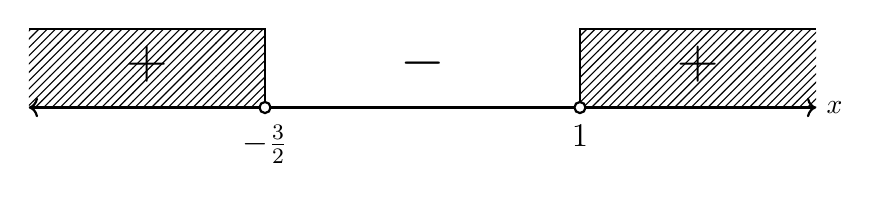
\begin{tikzpicture}
    \draw[thick,<->] (-5,0) -- (5,0) node[right] {$x$};
    \fill[pattern=north east lines] (-5,0) rectangle (-2,1);
    \fill[pattern=north east lines] (2,0) rectangle (5,1);
    \draw[thick] (-5,1) -- (-2,1) -- (-2,0);
    \draw[thick] (2,0) -- (2,1) -- (5,1);
    \draw (-2,-0.1) node[below] {\large{$-\frac{3}{2}$}};
    \draw (2,-0.1) node[below] {\large{$1$}};
    \draw (-3.5,0.2) node[above] {\huge{$+$}};
    \draw (0,0.2) node[above] {\huge{$-$}};
    \draw (3.5,0.2) node[above] {\huge{$+$}};
    \draw[fill=white, thick] (-2,0) circle (2pt);
    \draw[fill=white, thick] (2,0) circle (2pt);
            \end{tikzpicture}
        \end{center}
        Pembuat nol penyebut tidak diikutkan karena membuat ekspresi tidak terdefinisi, dan karena pembilang tidak pernah nol, tidak ada titik yang membuat ekspresi sama dengan nol. Jadi himpunan penyelesaiannya adalah
        \[
        \colorlet{oldcolor}{.}
        \color{red}
        \setlength{\fboxrule}{1pt} \boxed{\color{oldcolor}\left(-\infty,-\frac{3}{2}\right)\cup\left(1,\infty\right)}\color{oldcolor}.
        \]
    }
    \end{jawab}

    \item \textbf{[Subbab 2.3]} Diberikan fungsi $f(x)=\begin{cases}
        2x+1, & x<1\\
        (x-2)^2, & x\geq 1
    \end{cases}$.
    \begin{enumerate}
        \item Dapatkan $f(1)$, $f(-3)$, dan $f(-x^2)$.
        \item Dapatkan domain dan range dari $f(x)$.
        \item Sketsa grafik dari $f(x)$.
    \end{enumerate}
    \begin{jawab}[fungsi sepotong-sepotong, domain dan range fungsi, sketsa grafik]{
        \begin{enumerate}
            \item Karena $1\geq 1$, digunakan rumus $(x-2)^2$. Karena $-3<1$, digunakan rumus $2x+1$. Selanjutnya, diperhatikan bahwa $-x^2\leq 0 < 1$ untuk setiap $x$, sehingga digunakan rumus $2x+1$. Diperoleh
            \begin{align*}
                f(1) &= (1-2)^2 = (-1)^2 = 1\\
                f(-3) &= 2(-3)+1 = -5\\
                f(-x^2) &= 2(-x^2)+1 = 1-2x^2.
            \end{align*}
            Jadi diperoleh $\colorlet{oldcolor}{.}
        \color{red}
        \setlength{\fboxrule}{1pt} \boxed{\color{oldcolor}f(1)=1,~f(-3)=-5,~f(-x^2)=1-2x^2}\color{oldcolor}$.
            \item Untuk $x<1$, $f(x)=2x+1$ adalah fungsi linear naik dengan domain $(-\infty,1)$ dan range $(-\infty,3)$. Untuk $x\geq 1$, $f(x)=(x-2)^2$ adalah fungsi kuadrat dengan nilai minimum $0$ di $x=2$, sehingga domainnya $[1,\infty)$ dan range-nya $[0,\infty)$. Dengan demikian, domain dari $f(x)$ adalah $\colorlet{oldcolor}{.}
        \color{red}
        \setlength{\fboxrule}{1pt} \boxed{\color{oldcolor}D(f)=(-\infty,1)\cup[1,\infty) = \mathbb{R}}\color{oldcolor}$, dan range dari $f(x)$ adalah $\colorlet{oldcolor}{.}
        \color{red}
        \setlength{\fboxrule}{1pt} \boxed{\color{oldcolor}R(f)=(-\infty,3)\cup[0,\infty) = \mathbb{R}}\color{oldcolor}$.
            \item Sketsa grafik dari $f(x)$ adalah sebagai berikut. Diperhatikan bahwa potongan garis berakhir di titik $(1,3)$ yang tidak termasuk grafik (bulatan kosong), sedangkan potongan parabola dimulai dari titik $(1,1)$ yang termasuk grafik (bulatan penuh).
            \begin{center}
                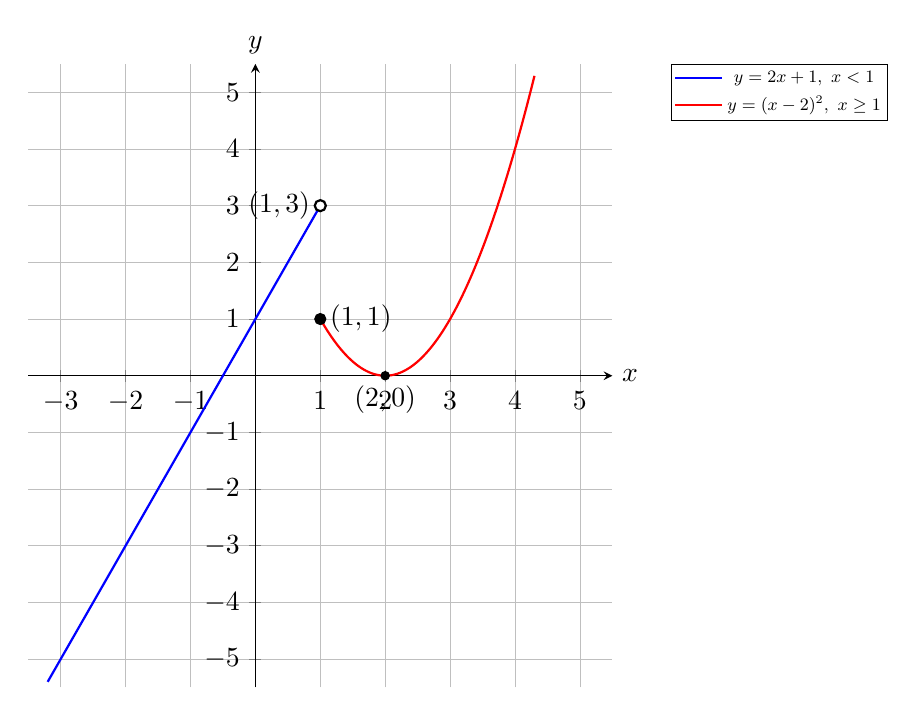
\begin{tikzpicture}
                    \begin{axis}[
        axis lines = middle,
        xlabel = $x$,
        ylabel = {$y$},
        grid=both,
        grid style={line width=.1pt, draw=gray!10},
        major grid style={line width=.2pt,draw=gray!50},
        x label style={anchor=west}, % label x ke kanan
        y label style={anchor=south}, % label y ke atas
        samples=200,
        legend style={
                at={(1.1,1)},
                anchor=north west,
                font=\small,         % mengecilkan ukuran font
                row sep=1pt,         % jarak antar baris legend
                inner sep=1pt,       % margin dalam kotak legend
                nodes={scale=0.7}    % skalakan isi legend
            },
        xtick={-3,-2,...,5},
        ytick={-5,-4,...,5},
        xmin=-3.5, xmax=5.5,
        ymin=-5.5, ymax=5.5,
        width=9cm,
        height=9.5cm
    ]
\addplot[domain=-3.2:1, color=blue, thick, samples=2] {2*x+1};
\addlegendentry{$y=2x+1,\ x<1$}
\addplot[domain=1:4.3, color=red, thick] {(x-2)^2};
\addlegendentry{$y=(x-2)^2,\ x\geq 1$}
\draw[fill=white, thick] (1,3) circle (2pt) node[left] {$(1,3)$};
\draw[fill=black] (1,1) circle (2pt) node[right] {$(1,1)$};
\draw[fill=black] (2,0) circle (1.5pt) node[below] {$(2,0)$};
\end{axis}
                \end{tikzpicture}
            \end{center}
        \end{enumerate}
    }
    \end{jawab}

    \item \textbf{[Subbab 2.4]} Diberikan fungsi $f(x)=\sqrt{4x-x^2},\ 0\leq x\leq 2$.
    \begin{enumerate}
        \item Tentukan $f^{-1}(x)$ beserta domainnya.
        \item Gambarkan grafik $f(x)$ dan $f^{-1}(x)$ dalam satu bidang koordinat.
    \end{enumerate}
    \begin{jawab}[melengkapkan kuadrat, setengah lingkaran, fungsi invers, sketsa grafik fungsi invers]{
        \begin{enumerate}
            \item Dengan melengkapkan kuadrat, diperoleh $4x-x^2 = 4-(x^2-4x+4) = \colorlet{oldcolor}{.}
        \color{blue}
        \setlength{\fboxrule}{1pt} \boxed{\color{oldcolor}4-(x-2)^2}\color{oldcolor}$, sehingga $f(x)=\sqrt{4-(x-2)^2}$. Grafik $f$ adalah bagian dari setengah lingkaran atas $(x-2)^2+y^2=4$ dengan pusat $(2,0)$ dan jari-jari $2$. Pada $0\leq x\leq 2$, fungsi $f$ naik dari $f(0)=0$ sampai $f(2)=2$, sehingga $f$ satu-satu dan $R(f)=[0,2]$.\\
            Misalkan $y=f(x)$ dengan $0\leq x\leq 2$, kemudian selesaikan sehingga terbentuk $x$ dalam fungsi $y$. Diperoleh
            \begin{align*}
                y &= \sqrt{4-(x-2)^2}\\
                y^2 &= 4-(x-2)^2\\
                (x-2)^2 &= 4-y^2\\
                x-2 &= -\sqrt{4-y^2} \quad (\text{karena } x\leq 2, \text{ yaitu } x-2\leq 0)\\
                x &= 2-\sqrt{4-y^2}.
            \end{align*}
            Dari sini didapatkan $x = f^{-1}(y) = 2-\sqrt{4-y^2}$. Dengan mengganti $y$ dengan $x$, dan mengingat bahwa domain dari fungsi invers adalah range dari fungsi asli, diperoleh
            \begin{align*}
                \colorlet{oldcolor}{.}
        \color{red}
        \setlength{\fboxrule}{1pt} \boxed{\color{oldcolor}f^{-1}(x) = 2-\sqrt{4-x^2},\quad D(f^{-1})=R(f)=[0,2]}\color{oldcolor}.
            \end{align*}
            \item Grafik $f$ adalah seperempat lingkaran berpusat di $(2,0)$ dari titik $(0,0)$ ke $(2,2)$. Grafik $f^{-1}$ merupakan pencerminan grafik $f$ terhadap garis $y=x$, yaitu seperempat lingkaran $x^2+(y-2)^2=4$ yang berpusat di $(0,2)$, juga dari titik $(0,0)$ ke $(2,2)$. Sketsa grafiknya adalah sebagai berikut.
            \begin{center}
                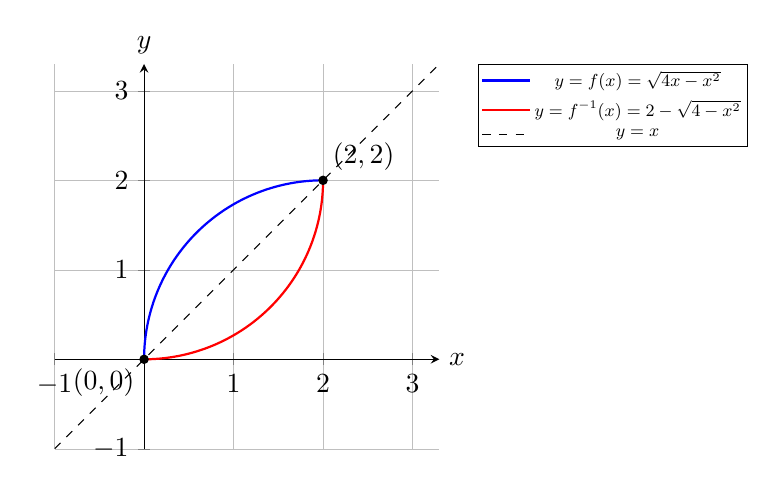
\begin{tikzpicture}
                    \begin{axis}[
        axis lines = middle,
        xlabel = $x$,
        ylabel = {$y$},
        grid=both,
        grid style={line width=.1pt, draw=gray!10},
        major grid style={line width=.2pt,draw=gray!50},
        x label style={anchor=west}, % label x ke kanan
        y label style={anchor=south}, % label y ke atas
        samples=200,
        legend style={
                at={(1.1,1)},
                anchor=north west,
                font=\small,         % mengecilkan ukuran font
                row sep=1pt,         % jarak antar baris legend
                inner sep=1pt,       % margin dalam kotak legend
                nodes={scale=0.7}    % skalakan isi legend
            },
        xtick={-1,0,...,3},
        ytick={-1,0,...,3},
        xmin=-1, xmax=3.3,
        ymin=-1, ymax=3.3,
        axis equal image,
        width=7.5cm
    ]
\addplot[domain=90:180, color=blue, thick] ({2+2*cos(x)}, {2*sin(x)});
\addlegendentry{$y=f(x)=\sqrt{4x-x^2}$}
\addplot[domain=90:180, color=red, thick] ({2*sin(x)}, {2+2*cos(x)});
\addlegendentry{$y=f^{-1}(x)=2-\sqrt{4-x^2}$}
\addplot[domain=-1:3.3, color=black, dashed, samples=2] {x};
\addlegendentry{$y=x$}
\draw[fill=black] (0,0) circle (1.5pt) node[below left] {$(0,0)$};
\draw[fill=black] (2,2) circle (1.5pt) node[above right] {$(2,2)$};
\end{axis}
                \end{tikzpicture}
            \end{center}
        \end{enumerate}
    }
    \end{jawab}

    \item \textbf{[Subbab 3.3]} Hitunglah $\displaystyle\lim_{x\to+\infty}\frac{3x^2-2x}{\sqrt{x^4+1}}$.
    \begin{jawab}[limit di tak hingga, bentuk akar]{~\\
        Jika $x\to+\infty$, diperoleh bentuk tak tentu $\frac{\infty}{\infty}$. Diperhatikan bahwa $\sqrt{x^4}=x^2$, sehingga pembilang dan penyebut dibagi dengan $\colorlet{oldcolor}{.}
        \color{blue}
        \setlength{\fboxrule}{1pt} \boxed{\color{oldcolor}x^2=\sqrt{x^4}}\color{oldcolor}$. Diperoleh
        \begin{align*}
            \lim_{x\to+\infty}\frac{3x^2-2x}{\sqrt{x^4+1}} &= \lim_{x\to+\infty}\frac{\frac{3x^2-2x}{x^2}}{\frac{\sqrt{x^4+1}}{\sqrt{x^4}}}\\
            &= \lim_{x\to+\infty}\frac{3-\frac{2}{x}}{\sqrt{1+\frac{1}{x^4}}}\\
            &= \frac{3-0}{\sqrt{1+0}}\\
            &= \colorlet{oldcolor}{.}
        \color{red}
        \setlength{\fboxrule}{1pt} \boxed{\color{oldcolor}3}\color{oldcolor}.
        \end{align*}
    }
    \end{jawab}

    \item \textbf{[Subbab 4.4]} Diketahui garis singgung pada kurva $x^2-xy+y^2=12$ di titik $(a,b)$ sejajar dengan sumbu-$x$. Tentukan semua titik $(a,b)$ dan persamaan garis singgungnya.
    \begin{jawab}[turunan implisit, garis singgung mendatar, persamaan garis singgung]{~\\
        Garis yang sejajar dengan sumbu-$x$ memiliki gradien nol, sehingga di titik $(a,b)$ haruslah $\colorlet{oldcolor}{.}
        \color{blue}
        \setlength{\fboxrule}{1pt} \boxed{\color{oldcolor}\frac{dy}{dx}=0}\color{oldcolor}$. Kita turunkan kedua ruas persamaan kurva terhadap $x$, dengan aturan perkalian $\frac{d}{dx}(xy)=y+x\frac{dy}{dx}$ dan aturan rantai $\frac{d}{dx}(y^2)=2y\frac{dy}{dx}$:
        \begin{align*}
            2x - \left(y + x\frac{dy}{dx}\right) + 2y\frac{dy}{dx} &= 0\\
            (2y - x)\frac{dy}{dx} &= y - 2x\\
            \frac{dy}{dx} &= \colorlet{oldcolor}{.}
        \color{blue}
        \setlength{\fboxrule}{1pt} \boxed{\color{oldcolor}\frac{y-2x}{2y-x}}\color{oldcolor}.
        \end{align*}
        Agar $\frac{dy}{dx}=0$ di titik $(a,b)$, haruslah pembilangnya nol (dengan penyebut tidak nol), yaitu $b-2a=0$ atau $\colorlet{oldcolor}{.}
        \color{blue}
        \setlength{\fboxrule}{1pt} \boxed{\color{oldcolor}b=2a}\color{oldcolor}$. Karena titik $(a,b)$ terletak pada kurva, substitusi $b=2a$ ke persamaan kurva:
        \begin{align*}
            a^2 - a(2a) + (2a)^2 &= 12\\
            a^2 - 2a^2 + 4a^2 &= 12\\
            3a^2 &= 12\\
            a^2 &= 4 \implies a=\pm 2.
        \end{align*}
        Untuk $a=2$ diperoleh $b=4$, dan untuk $a=-2$ diperoleh $b=-4$. Dicek penyebutnya, yaitu $2(4)-2=6\neq 0$ dan $2(-4)-(-2)=-6\neq 0$. Jadi titik-titik yang dimaksud adalah $\colorlet{oldcolor}{.}
        \color{red}
        \setlength{\fboxrule}{1pt} \boxed{\color{oldcolor}(2,4) \text{ dan } (-2,-4)}\color{oldcolor}$.\\
        Garis singgung yang sejajar sumbu-$x$ berbentuk $y=b$, sehingga persamaan garis singgungnya adalah
        \begin{align*}
            \colorlet{oldcolor}{.}
        \color{red}
        \setlength{\fboxrule}{1pt} \boxed{\color{oldcolor}y=4 \text{ (di titik } (2,4)) \quad\text{dan}\quad y=-4 \text{ (di titik } (-2,-4))}\color{oldcolor}.
        \end{align*}
    }
    \end{jawab}
\end{enumerate}

\newpage

%%%%%%%%%%%%%%%%%%%%%%%%%%%%%%%%%%%%%%%%%%%%%%%%%%%%%%%%%%%%%%%%%%%%%%%%%%%%%%
% Kal-iup-2
% Kisi-kisi hari Senin: subbab 1.1, 1.5, 2.3, 2.4, 3.1, 3.3, 4.2, 4.4
\kopsoaliup{Kal-iup-2}{62, 69}{Mechanical, Industrial, Materials \& Metallurgical Engineering}{Monday, Wednesday; 15.30-17.10}{4}
\begin{enumerate}
    \item \textbf{[Subbab 1.1]} Find the solution of the following inequality
    \begin{align*}
        \frac{x^2+x-6}{x^2-3x-4}\geq 0.
    \end{align*}
    \begin{jawab}[pertidaksamaan rasional, faktorisasi, garis bilangan, notasi interval]{~\\
    Karena ruas kanan pertidaksamaan sudah bernilai nol, maka kita bisa langsung memfaktorkan pembilang dan penyebut di ruas kiri. Diperoleh
    \begin{align*}
        \frac{x^2+x-6}{x^2-3x-4} = \frac{(x+3)(x-2)}{(x-4)(x+1)} \geq 0.
    \end{align*}
    Selanjutnya, kita tentukan pembuat nol dari faktor-faktor tersebut, yaitu
    \begin{align*}
        x+3 = 0 \quad &\vee\quad x-2 = 0 \quad \vee\quad x-4 = 0 \quad \vee\quad x+1 = 0\\
        \colorlet{oldcolor}{.}
        \color{blue}
        \setlength{\fboxrule}{1pt} \boxed{\color{oldcolor}x=-3}\color{oldcolor} \quad &\vee\quad \colorlet{oldcolor}{.}
        \color{blue}
        \setlength{\fboxrule}{1pt} \boxed{\color{oldcolor}x=2}\color{oldcolor} \quad \vee\quad \colorlet{oldcolor}{.}
        \color{blue}
        \setlength{\fboxrule}{1pt} \boxed{\color{oldcolor}x=4}\color{oldcolor} \quad \vee\quad \colorlet{oldcolor}{.}
        \color{blue}
        \setlength{\fboxrule}{1pt} \boxed{\color{oldcolor}x=-1}\color{oldcolor}
    \end{align*}
    Selanjutnya, kita buat garis bilangan dan lakukan uji titik pada ekspresi \(\frac{(x+3)(x-2)}{(x-4)(x+1)}\) sebagai berikut
    \begin{itemize}
        \item Untuk \(x < -3\), misalkan \(x = -4\):
        \[
        \frac{(-4+3)(-4-2)}{(-4-4)(-4+1)} = \frac{(-1)(-6)}{(-8)(-3)} = \frac{6}{24} > 0
        \]
        \item Untuk \(-3 < x < -1\), misalkan \(x = -2\):
        \[
        \frac{(-2+3)(-2-2)}{(-2-4)(-2+1)} = \frac{(1)(-4)}{(-6)(-1)} = \frac{-4}{6} < 0
        \]
        \item Untuk \(-1 < x < 2\), misalkan \(x = 0\):
        \[
        \frac{(0+3)(0-2)}{(0-4)(0+1)} = \frac{(3)(-2)}{(-4)(1)} = \frac{6}{4} > 0
        \]
        \item Untuk \(2 < x < 4\), misalkan \(x = 3\):
        \[
        \frac{(3+3)(3-2)}{(3-4)(3+1)} = \frac{(6)(1)}{(-1)(4)} = \frac{-6}{4} < 0
        \]
        \item Untuk \(x > 4\), misalkan \(x = 5\):
        \[
        \frac{(5+3)(5-2)}{(5-4)(5+1)} = \frac{(8)(3)}{(1)(6)} = 4 > 0
        \]
    \end{itemize}
    \begin{center}
        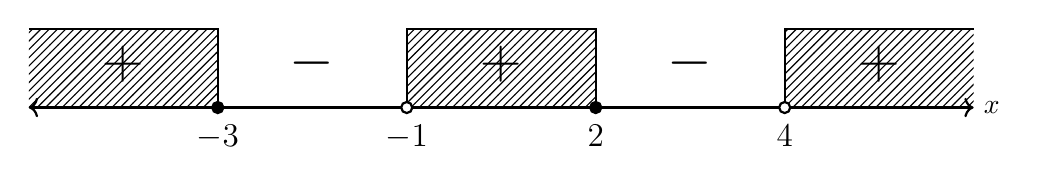
\begin{tikzpicture}
    \draw[thick,<->] (-6,0) -- (6,0) node[right] {$x$};
    \fill[pattern=north east lines] (-6,0) rectangle (-3.6,1);
    \fill[pattern=north east lines] (-1.2,0) rectangle (1.2,1);
    \fill[pattern=north east lines] (3.6,0) rectangle (6,1);
    \draw[thick] (-6,1) -- (-3.6,1) -- (-3.6,0);
    \draw[thick] (-1.2,0) -- (-1.2,1) -- (1.2,1) -- (1.2,0);
    \draw[thick] (3.6,0) -- (3.6,1) -- (6,1);
    \draw (-3.6,-0.1) node[below] {\large{$-3$}};
    \draw (-1.2,-0.1) node[below] {\large{$-1$}};
    \draw (1.2,-0.1) node[below] {\large{$2$}};
    \draw (3.6,-0.1) node[below] {\large{$4$}};
    \draw (-4.8,0.2) node[above] {\huge{$+$}};
    \draw (-2.4,0.2) node[above] {\huge{$-$}};
    \draw (0,0.2) node[above] {\huge{$+$}};
    \draw (2.4,0.2) node[above] {\huge{$-$}};
    \draw (4.8,0.2) node[above] {\huge{$+$}};
    \draw[fill=black, thick] (-3.6,0) circle (2pt);
    \draw[fill=white, thick] (-1.2,0) circle (2pt);
    \draw[fill=black, thick] (1.2,0) circle (2pt);
    \draw[fill=white, thick] (3.6,0) circle (2pt);
        \end{tikzpicture}
    \end{center}
    Karena yang diminta adalah nilai yang lebih dari atau sama dengan nol, diambil interval yang bertanda positif beserta pembuat nol dari pembilang ($x=-3$ dan $x=2$). Pembuat nol dari penyebut ($x=-1$ dan $x=4$) tidak diikutkan karena membuat ekspresi tidak terdefinisi. Jadi solusi dari pertidaksamaan tersebut adalah \(x \leq -3\) atau \(-1 < x \leq 2\) atau \(x > 4\). Dalam notasi interval, solusi tersebut dapat ditulis sebagai $\colorlet{oldcolor}{.}
        \color{red}
        \setlength{\fboxrule}{1pt} \boxed{\color{oldcolor}(-\infty, -3] \cup (-1, 2] \cup (4, \infty)}\color{oldcolor}$.
    }
    \end{jawab}

    \item \textbf{[Subbab 1.5]} Given the circle $x^2+y^2+4x-2y-4=0$.
    \begin{enumerate}
        \item Find the center and the radius of the circle.
        \item Find the equation of the lower half of the circle in the form $y=f(x)$, then sketch its graph.
    \end{enumerate}
    \begin{jawab}[persamaan lingkaran, melengkapkan kuadrat, setengah lingkaran, sketsa grafik]{
        \begin{enumerate}
            \item Persamaan lingkaran diubah ke bentuk baku dengan cara melengkapkan kuadrat, yaitu
            \begin{align*}
                x^2+4x+y^2-2y &= 4\\
                (x^2+4x+4)+(y^2-2y+1) &= 4+4+1\\
                (x+2)^2+(y-1)^2 &= 9.
            \end{align*}
            Jadi pusat dan jari-jari lingkaran adalah $\colorlet{oldcolor}{.}
        \color{red}
        \setlength{\fboxrule}{1pt} \boxed{\color{oldcolor}\text{Pusat: }(-2,1),~\text{Jari-jari: }3}\color{oldcolor}$.
            \item Dari bentuk baku, diperoleh
            \begin{align*}
                (y-1)^2 &= 9-(x+2)^2\\
                y-1 &= \pm\sqrt{9-(x+2)^2}\\
                y &= 1\pm\sqrt{9-(x+2)^2}.
            \end{align*}
            Tanda $+$ menghasilkan bagian atas lingkaran ($y\geq 1$), sedangkan tanda $-$ menghasilkan bagian bawah lingkaran ($y\leq 1$). Karena $9-(x+2)^2=9-x^2-4x-4=5-4x-x^2$, persamaan setengah lingkaran bagian bawah adalah
            \begin{align*}
                \colorlet{oldcolor}{.}
        \color{red}
        \setlength{\fboxrule}{1pt} \boxed{\color{oldcolor}y=1-\sqrt{5-4x-x^2},\quad -5\leq x\leq 1}\color{oldcolor}.
            \end{align*}
            Grafiknya adalah setengah lingkaran bagian bawah dengan ujung-ujung $(-5,1)$ dan $(1,1)$ serta titik terendah $(-2,-2)$. Sketsa grafiknya adalah sebagai berikut:
            \begin{center}
                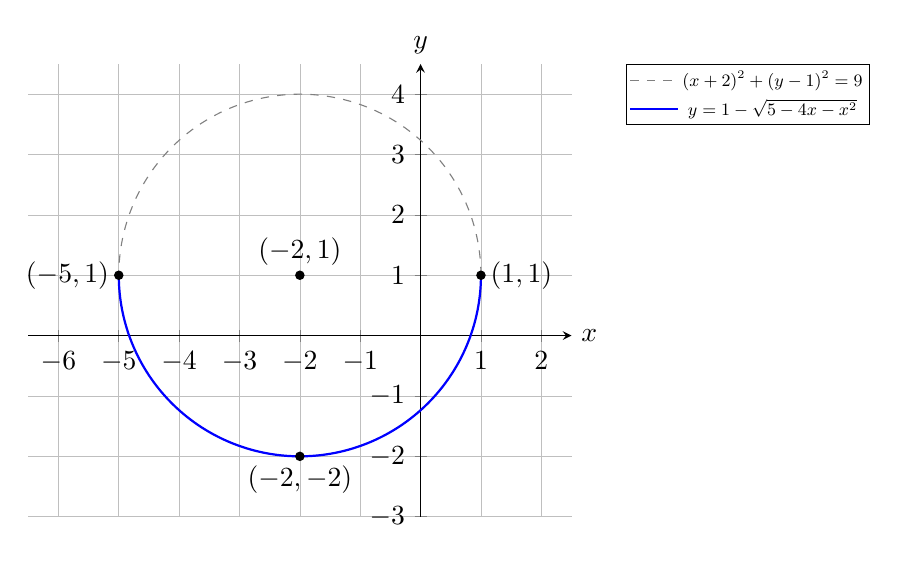
\begin{tikzpicture}
                    \begin{axis}[
        axis lines = middle,
        xlabel = $x$,
        ylabel = {$y$},
        grid=both,
        grid style={line width=.1pt, draw=gray!10},
        major grid style={line width=.2pt,draw=gray!50},
        x label style={anchor=west}, % label x ke kanan
        y label style={anchor=south}, % label y ke atas
        samples=200,
        legend style={
                at={(1.1,1)},
                anchor=north west,
                font=\small,         % mengecilkan ukuran font
                row sep=1pt,         % jarak antar baris legend
                inner sep=1pt,       % margin dalam kotak legend
                nodes={scale=0.7}    % skalakan isi legend
            },
        xtick={-6,-5,...,2},
        ytick={-3,-2,...,4},
        xmin=-6.5, xmax=2.5,
        ymin=-3, ymax=4.5,
        axis equal image,
        width=8.5cm
    ]
\addplot[domain=0:360, color=gray, dashed] ({-2+3*cos(x)}, {1+3*sin(x)});
\addlegendentry{$(x+2)^2+(y-1)^2=9$}
\addplot[domain=180:360, color=blue, thick] ({-2+3*cos(x)}, {1+3*sin(x)});
\addlegendentry{$y=1-\sqrt{5-4x-x^2}$}
\draw[fill=black] (-2,1) circle (1.5pt) node[above] {$(-2,1)$};
\draw[fill=black] (-5,1) circle (1.5pt) node[left] {$(-5,1)$};
\draw[fill=black] (1,1) circle (1.5pt) node[right] {$(1,1)$};
\draw[fill=black] (-2,-2) circle (1.5pt) node[below] {$(-2,-2)$};
\end{axis}
                \end{tikzpicture}
            \end{center}
        \end{enumerate}
    }
    \end{jawab}

    \item \textbf{[Subbab 4.4]} Write the chain rule formula for $\dfrac{d}{dx}\big[f(g(x))\big]$.\\
    Then, find the derivative of $h(x)=\left(2x^3-x\right)^4$.
    \begin{jawab}[turunan, aturan rantai]{~\\
        Ingat kembali aturan rantai untuk turunan fungsi komposisi, yaitu
        \[
        \colorlet{oldcolor}{.}
        \color{red}
        \setlength{\fboxrule}{1pt} \boxed{\color{oldcolor}\frac{d}{dx}\big[f(g(x))\big] = f'(g(x)) \cdot g'(x)}\color{oldcolor}.
        \]
        Dapat dimisalkan $\colorlet{oldcolor}{.}
        \color{blue}
        \setlength{\fboxrule}{1pt} \boxed{\color{oldcolor}u=g(x)=2x^3-x}\color{oldcolor}$ sehingga $\colorlet{oldcolor}{.}
        \color{blue}
        \setlength{\fboxrule}{1pt} \boxed{\color{oldcolor}f(u)=u^4}\color{oldcolor}$, dan diperoleh
        \begin{align*}
            \colorlet{oldcolor}{.}
        \color{blue}
        \setlength{\fboxrule}{1pt} \boxed{\color{oldcolor}f'(u)=4u^3}\color{oldcolor} \quad\text{dan}\quad \colorlet{oldcolor}{.}
        \color{blue}
        \setlength{\fboxrule}{1pt} \boxed{\color{oldcolor}g'(x)=6x^2-1}\color{oldcolor}.
        \end{align*}
        Dengan demikian, diperoleh
        \begin{align*}
            h'(x) = \colorlet{oldcolor}{.}
        \color{red}
        \setlength{\fboxrule}{1pt} \boxed{\color{oldcolor}4\left(2x^3-x\right)^3\left(6x^2-1\right)}\color{oldcolor}.
        \end{align*}
    }
    \end{jawab}

    \item \textbf{[Subbab 3.3]} Calculate $\displaystyle\lim_{x\to-\infty}\frac{\sqrt{9x^2+2}}{1-3x}$.
    \begin{jawab}[limit di tak hingga, bentuk akar, nilai mutlak]{~\\
        Diperhatikan bahwa jika $x\to-\infty$, diperoleh bentuk tak tentu $\frac{\infty}{\infty}$. Keluarkan $x^2$ dari dalam akar dengan mengingat bahwa $\colorlet{oldcolor}{.}
        \color{blue}
        \setlength{\fboxrule}{1pt} \boxed{\color{oldcolor}\sqrt{x^2}=|x|}\color{oldcolor}$, dan karena $x\to-\infty$ (yaitu $x<0$), maka $\colorlet{oldcolor}{.}
        \color{blue}
        \setlength{\fboxrule}{1pt} \boxed{\color{oldcolor}|x|=-x}\color{oldcolor}$. Diperoleh
        \begin{align*}
            \lim_{x\to-\infty}\frac{\sqrt{9x^2+2}}{1-3x} &= \lim_{x\to-\infty}\frac{-x\sqrt{9+\frac{2}{x^2}}}{-x\left(3-\frac{1}{x}\right)}\\
            &= \lim_{x\to-\infty}\frac{\sqrt{9+\frac{2}{x^2}}}{3-\frac{1}{x}}\\
            &= \frac{\sqrt{9+0}}{3-0}\\
            &= \colorlet{oldcolor}{.}
        \color{red}
        \setlength{\fboxrule}{1pt} \boxed{\color{oldcolor}1}\color{oldcolor}.
        \end{align*}
    }
    \end{jawab}

    \item \textbf{[Subbab 2.4]} Given a function $f(x)=\dfrac{2x+1}{x-3}$.
    \begin{enumerate}
        \item Find the domain and range of $f$.
        \item Find $f^{-1}(x)$ and its domain.
        \item Verify that $\left(f\circ f^{-1}\right)(x)=x$.
    \end{enumerate}
    \begin{jawab}[domain dan range fungsi rasional, fungsi invers, fungsi komposisi]{
        \begin{enumerate}
            \item Fungsi $f$ terdefinisi jika $x-3\neq 0$, sehingga $\colorlet{oldcolor}{.}
        \color{red}
        \setlength{\fboxrule}{1pt} \boxed{\color{oldcolor}D(f)=\mathbb{R}\setminus\{3\}}\color{oldcolor}$. Untuk menentukan range, misalkan $y=\frac{2x+1}{x-3}$ dan selesaikan untuk $x$:
            \begin{align*}
                y(x-3) &= 2x+1\\
                yx-2x &= 3y+1\\
                x(y-2) &= 3y+1\\
                x &= \frac{3y+1}{y-2}.
            \end{align*}
            Nilai $x$ tersebut ada untuk setiap $y\neq 2$ (untuk $y=2$ diperoleh $0=7$, yang tidak mungkin). Jadi $\colorlet{oldcolor}{.}
        \color{red}
        \setlength{\fboxrule}{1pt} \boxed{\color{oldcolor}R(f)=\mathbb{R}\setminus\{2\}}\color{oldcolor}$.
            \item Dari perhitungan di (a), diperoleh $x=f^{-1}(y)=\frac{3y+1}{y-2}$. Dengan mengganti $y$ dengan $x$, dan mengingat bahwa domain dari fungsi invers adalah range dari fungsi asli, diperoleh
            \begin{align*}
                \colorlet{oldcolor}{.}
        \color{red}
        \setlength{\fboxrule}{1pt} \boxed{\color{oldcolor}f^{-1}(x)=\frac{3x+1}{x-2},\quad D(f^{-1})=R(f)=\mathbb{R}\setminus\{2\}}\color{oldcolor}.
            \end{align*}
            \item Untuk $x\neq 2$, diperoleh
            \begin{align*}
                \left(f\circ f^{-1}\right)(x) = f\left(\frac{3x+1}{x-2}\right) = \frac{2\cdot\frac{3x+1}{x-2}+1}{\frac{3x+1}{x-2}-3} = \frac{\frac{6x+2+x-2}{x-2}}{\frac{3x+1-3x+6}{x-2}} = \frac{7x}{7} = \colorlet{oldcolor}{.}
        \color{red}
        \setlength{\fboxrule}{1pt} \boxed{\color{oldcolor}x}\color{oldcolor}.
            \end{align*}
            Jadi terbukti bahwa $\left(f\circ f^{-1}\right)(x)=x$ untuk setiap $x$ pada domain $f^{-1}$.
        \end{enumerate}
    }
    \end{jawab}

\end{enumerate}

\newpage

%%%%%%%%%%%%%%%%%%%%%%%%%%%%%%%%%%%%%%%%%%%%%%%%%%%%%%%%%%%%%%%%%%%%%%%%%%%%%%
% Kal-3
% Kisi-kisi hari Selasa: subbab 1.2, 1.4, 2.1, 2.2, 3.2, 3.4, 4.2, 4.3
\kopsoal{Kal-3}{13-16}{Kimia, Saik, Telkom}{Selasa, Kamis; 07.00-09.30}{6}
\begin{enumerate}
    \item \textbf{[Subbab 1.2]} Tentukan himpunan penyelesaian dari persamaan
    \begin{align*}
        |x+1|+2x=|x-3|+4.
    \end{align*}
    \begin{jawab}[definisi nilai mutlak, persamaan nilai mutlak, pembagian kasus]{~\\
        Ingat kembali definisi nilai mutlak, yaitu
        \begin{align*}
            |x+1| = \begin{cases}
                x+1, & x\geq -1\\
                -(x+1), & x<-1
            \end{cases}
            \quad\text{dan}\quad
            |x-3| = \begin{cases}
                x-3, & x\geq 3\\
                -(x-3), & x<3
            \end{cases}.
        \end{align*}
        Titik-titik batasnya adalah $\colorlet{oldcolor}{.}
        \color{blue}
        \setlength{\fboxrule}{1pt} \boxed{\color{oldcolor}x=-1}\color{oldcolor}$ dan $\colorlet{oldcolor}{.}
        \color{blue}
        \setlength{\fboxrule}{1pt} \boxed{\color{oldcolor}x=3}\color{oldcolor}$, sehingga garis bilangan terbagi menjadi tiga kasus.
        \begin{enumerate}
            \item[(i)] Jika $x<-1$, maka persamaan menjadi
            \begin{align*}
                -(x+1)+2x = -(x-3)+4 \iff x-1 = -x+7 \iff x=4.
            \end{align*}
            Namun $x=4$ tidak memenuhi syarat $x<-1$, sehingga $\colorlet{oldcolor}{.}
        \color{blue}
        \setlength{\fboxrule}{1pt} \boxed{\color{oldcolor}\text{tidak ada solusi}}\color{oldcolor}$ pada kasus ini.
            \item[(ii)] Jika $-1\leq x<3$, maka persamaan menjadi
            \begin{align*}
                (x+1)+2x = -(x-3)+4 \iff 3x+1 = -x+7 \iff 4x=6 \iff x=\frac{3}{2}.
            \end{align*}
            Karena $-1\leq\frac{3}{2}<3$, maka $\colorlet{oldcolor}{.}
        \color{blue}
        \setlength{\fboxrule}{1pt} \boxed{\color{oldcolor}x=\frac{3}{2}}\color{oldcolor}$ memenuhi.
            \item[(iii)] Jika $x\geq 3$, maka persamaan menjadi
            \begin{align*}
                (x+1)+2x = (x-3)+4 \iff 3x+1 = x+1 \iff x=0.
            \end{align*}
            Namun $x=0$ tidak memenuhi syarat $x\geq 3$, sehingga $\colorlet{oldcolor}{.}
        \color{blue}
        \setlength{\fboxrule}{1pt} \boxed{\color{oldcolor}\text{tidak ada solusi}}\color{oldcolor}$ pada kasus ini.
        \end{enumerate}
        Sebagai pengecekan, untuk $x=\frac{3}{2}$ diperoleh $\left|\frac{5}{2}\right|+3=\frac{11}{2}$ dan $\left|-\frac{3}{2}\right|+4=\frac{11}{2}$. Jadi himpunan penyelesaiannya adalah $\colorlet{oldcolor}{.}
        \color{red}
        \setlength{\fboxrule}{1pt} \boxed{\color{oldcolor}HP=\left\{\frac{3}{2}\right\}}\color{oldcolor}$.
    }
    \end{jawab}

    \item \textbf{[Subbab 2.2]} Tentukan domain dari fungsi $(f\circ g)(x)$ jika diketahui fungsi $g(x)=3x-1$ dengan $0\leq x<2$ dan fungsi $f$ terdefinisi pada interval $1\leq x<4$.
    \begin{jawab}[domain fungsi komposisi, pertidaksamaan linear]{~\\
        Dari soal diketahui bahwa $\colorlet{oldcolor}{.}
        \color{blue}
        \setlength{\fboxrule}{1pt} \boxed{\color{oldcolor}D(g)=[0,2)}\color{oldcolor}$ dan $\colorlet{oldcolor}{.}
        \color{blue}
        \setlength{\fboxrule}{1pt} \boxed{\color{oldcolor}D(f)=[1,4)}\color{oldcolor}$. Domain dari fungsi komposisi $f\circ g$ adalah semua nilai $x$ pada domain $g$ sehingga nilai dari $g(x)$ berada pada domain $f$, yang dapat dirumuskan sebagai
        \begin{align*}
            \colorlet{oldcolor}{.}
        \color{blue}
        \setlength{\fboxrule}{1pt} \boxed{\color{oldcolor}D(f\circ g) = \{x \in D(g) : g(x) \in D(f)\} = \{x \in [0,2) : 1\leq 3x-1<4\}}\color{oldcolor}.
        \end{align*}
        Selanjutnya, diselesaikan pertidaksamaan ganda $1\leq 3x-1<4$:
        \begin{align*}
            1\leq 3x-1<4 \iff 2\leq 3x<5 \iff \frac{2}{3}\leq x<\frac{5}{3}.
        \end{align*}
        Irisan dari $\left[\frac{2}{3},\frac{5}{3}\right)$ dengan $D(g)=[0,2)$ adalah $\left[\frac{2}{3},\frac{5}{3}\right)$, karena $0<\frac{2}{3}$ dan $\frac{5}{3}<2$. Jadi
        \begin{align*}
            \colorlet{oldcolor}{.}
        \color{red}
        \setlength{\fboxrule}{1pt} \boxed{\color{oldcolor}D(f\circ g) = \left\{x\in\mathbb{R} : \frac{2}{3}\leq x<\frac{5}{3}\right\} = \left[\frac{2}{3},\frac{5}{3}\right)}\color{oldcolor}.
        \end{align*}
    }
    \end{jawab}

    \item \textbf{[Subbab 1.4]} Dapatkan koordinat semua titik $P$ pada sumbu-$x$ sehingga garis yang melalui $A(2,3)$ dan $P$ tegak lurus dengan garis yang melalui $B(9,2)$ dan $P$.
    \begin{jawab}[gradien garis, garis tegak lurus, persamaan kuadrat]{~\\
        Karena $P$ terletak pada sumbu-$x$, misalkan $\colorlet{oldcolor}{.}
        \color{blue}
        \setlength{\fboxrule}{1pt} \boxed{\color{oldcolor}P(p,0)}\color{oldcolor}$. Kemiringan garis yang melalui dua titik $(x_1,y_1)$ dan $(x_2,y_2)$ adalah $m = \frac{y_2 - y_1}{x_2 - x_1}$, sehingga
        \begin{align*}
            m_{AP} = \frac{0-3}{p-2} = \frac{-3}{p-2} \quad\text{dan}\quad m_{BP} = \frac{0-2}{p-9} = \frac{-2}{p-9},
        \end{align*}
        dengan $p\neq 2$ dan $p\neq 9$. Dua garis saling tegak lurus jika $\colorlet{oldcolor}{.}
        \color{blue}
        \setlength{\fboxrule}{1pt} \boxed{\color{oldcolor}m_{AP}\cdot m_{BP}=-1}\color{oldcolor}$, sehingga
        \begin{align*}
            \frac{-3}{p-2}\cdot\frac{-2}{p-9} &= -1\\
            6 &= -(p-2)(p-9)\\
            6 &= -(p^2-11p+18)\\
            p^2-11p+24 &= 0\\
            (p-3)(p-8) &= 0,
        \end{align*}
        sehingga $p=3$ atau $p=8$. Sebagai pengecekan, untuk $P(3,0)$ diperoleh $m_{AP}=-3$ dan $m_{BP}=\frac{1}{3}$, sedangkan untuk $P(8,0)$ diperoleh $m_{AP}=-\frac{1}{2}$ dan $m_{BP}=2$; keduanya memenuhi $m_{AP}\cdot m_{BP}=-1$. Jadi titik-titik yang dimaksud adalah $\colorlet{oldcolor}{.}
        \color{red}
        \setlength{\fboxrule}{1pt} \boxed{\color{oldcolor}P(3,0) \text{ dan } P(8,0)}\color{oldcolor}$.
    }
    \end{jawab}

    \item \textbf{[Subbab 3.2]} Diberikan $f(x)=\begin{cases}
        k^2(x-1), & x\leq 2\\
        k(x+1), & x>2
    \end{cases}$.\\
    Tentukan semua nilai $k$ yang memenuhi agar $\displaystyle\lim_{x\to 2}f(x)$ ada.
    \begin{jawab}[limit sepihak, fungsi sepotong-sepotong, persamaan kuadrat]{~\\
        Ingat kembali bahwa $\displaystyle\lim_{x\to a}f(x)$ ada jika dan hanya jika limit kiri dan limit kanannya ada dan bernilai sama, yaitu $\colorlet{oldcolor}{.}
        \color{blue}
        \setlength{\fboxrule}{1pt} \boxed{\color{oldcolor}\lim_{x \to a^-} f(x) = \lim_{x \to a^+} f(x)}\color{oldcolor}$. Untuk $x\to 2^-$ (yaitu $x<2$) digunakan rumus $k^2(x-1)$, dan untuk $x\to 2^+$ (yaitu $x>2$) digunakan rumus $k(x+1)$. Diperoleh
        \begin{align*}
            \lim_{x\to 2^-} f(x) = \lim_{x\to 2^-} k^2(x-1) = k^2 \quad\text{dan}\quad \lim_{x\to 2^+} f(x) = \lim_{x\to 2^+} k(x+1) = 3k.
        \end{align*}
        Agar limitnya ada, haruslah
        \begin{align*}
            k^2 &= 3k\\
            k^2-3k &= 0\\
            k(k-3) &= 0,
        \end{align*}
        sehingga $k=0$ atau $k=3$. Jadi semua nilai $k$ yang memenuhi adalah $\colorlet{oldcolor}{.}
        \color{red}
        \setlength{\fboxrule}{1pt} \boxed{\color{oldcolor}k=0 \text{ atau } k=3}\color{oldcolor}$.\\
        Sebagai pengecekan, untuk $k=0$ kedua limit sepihak bernilai $0$, sedangkan untuk $k=3$ kedua limit sepihak bernilai $9$.
    }
    \end{jawab}

    \item \textbf{[Subbab 4.3]} Dapatkan $f'(t)$ jika $f(t)=\dfrac{3t^2+t}{t^2-t}$.
    \begin{jawab}[turunan, aturan pembagian]{~\\
        Ingat kembali aturan turunan untuk pembagian fungsi, yaitu
        \[
        \colorlet{oldcolor}{.}
        \color{blue}
        \setlength{\fboxrule}{1pt} \boxed{\color{oldcolor}\left(\frac{u}{v}\right)' = \frac{u'v - uv'}{v^2}}\color{oldcolor}.
        \]
        Misalkan $u=3t^2+t$ dan $v=t^2-t$, maka $\colorlet{oldcolor}{.}
        \color{blue}
        \setlength{\fboxrule}{1pt} \boxed{\color{oldcolor}u'=6t+1}\color{oldcolor}$ dan $\colorlet{oldcolor}{.}
        \color{blue}
        \setlength{\fboxrule}{1pt} \boxed{\color{oldcolor}v'=2t-1}\color{oldcolor}$. Diperoleh
        \begin{align*}
            f'(t) &= \frac{(6t+1)(t^2-t)-(3t^2+t)(2t-1)}{(t^2-t)^2}\\
            &= \frac{(6t^3-6t^2+t^2-t)-(6t^3-3t^2+2t^2-t)}{(t^2-t)^2}\\
            &= \frac{(6t^3-5t^2-t)-(6t^3-t^2-t)}{(t^2-t)^2}\\
            &= \frac{-4t^2}{t^2(t-1)^2}\\
            &= \colorlet{oldcolor}{.}
        \color{red}
        \setlength{\fboxrule}{1pt} \boxed{\color{oldcolor}-\frac{4}{(t-1)^2}}\color{oldcolor}, \quad t\neq 0,~t\neq 1.
        \end{align*}
        Hasil ini juga dapat dicek dengan menyederhanakan terlebih dahulu, yaitu $f(t)=\frac{t(3t+1)}{t(t-1)}=\frac{3t+1}{t-1}$ untuk $t\neq 0$, sehingga $f'(t)=\frac{3(t-1)-(3t+1)}{(t-1)^2}=-\frac{4}{(t-1)^2}$.
    }
    \end{jawab}

\end{enumerate}

\newpage

%%%%%%%%%%%%%%%%%%%%%%%%%%%%%%%%%%%%%%%%%%%%%%%%%%%%%%%%%%%%%%%%%%%%%%%%%%%%%%
% Kal-4
% Kisi-kisi hari Selasa: subbab 1.2, 1.4, 2.1, 2.2, 3.2, 3.4, 4.2, 4.3
\kopsoal{Kal-4}{17-21}{T. Mesin, Teknik Sistem dan Industri}{Selasa, Kamis; 07.00-09.30}{6}
\begin{enumerate}
    \item \textbf{[Subbab 1.2]} Tentukan semua nilai $x$ yang memenuhi
    \begin{align*}
        1<\frac{1}{|x-3|}\leq 2.
    \end{align*}
    \begin{jawab}[pertidaksamaan nilai mutlak, pertidaksamaan ganda, notasi interval]{~\\
        Agar bentuk $\frac{1}{|x-3|}$ terdefinisi, haruslah $\colorlet{oldcolor}{.}
        \color{blue}
        \setlength{\fboxrule}{1pt} \boxed{\color{oldcolor}x\neq 3}\color{oldcolor}$, sehingga $|x-3|>0$. Karena kedua ruas bernilai positif, membalik (mengambil kebalikan) setiap ruas akan membalik arah tanda pertidaksamaan, yaitu
        \begin{align*}
            1<\frac{1}{|x-3|}\leq 2 \iff \colorlet{oldcolor}{.}
        \color{blue}
        \setlength{\fboxrule}{1pt} \boxed{\color{oldcolor}\frac{1}{2}\leq |x-3|<1}\color{oldcolor}.
        \end{align*}
        Ingat kembali sifat nilai mutlak, yaitu untuk $a>0$ berlaku $|u|<a \iff -a<u<a$ dan $|u|\geq a \iff u\leq -a \;\vee\; u\geq a$. Pertidaksamaan tersebut dapat dipecah menjadi dua bagian:
        \begin{itemize}
            \item Untuk $|x-3|<1$, diperoleh
            \begin{align*}
                -1<x-3<1 \implies 2<x<4.
            \end{align*}
            \item Untuk $|x-3|\geq \frac{1}{2}$, diperoleh
            \begin{align*}
                x-3\leq -\frac{1}{2} \quad\vee\quad x-3\geq \frac{1}{2} \implies x\leq \frac{5}{2} \quad\vee\quad x\geq \frac{7}{2}.
            \end{align*}
        \end{itemize}
        Penyelesaiannya adalah irisan dari kedua bagian tersebut (yang otomatis memenuhi $x\neq 3$), yang dapat digambarkan pada garis bilangan sebagai berikut
        \begin{center}
            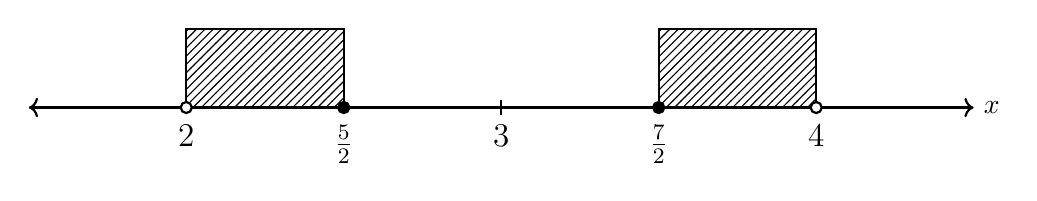
\begin{tikzpicture}
    \draw[thick,<->] (-6,0) -- (6,0) node[right] {$x$};
    \fill[pattern=north east lines] (-4,0) rectangle (-2,1);
    \fill[pattern=north east lines] (2,0) rectangle (4,1);
    \draw[thick] (-4,0) -- (-4,1) -- (-2,1) -- (-2,0);
    \draw[thick] (2,0) -- (2,1) -- (4,1) -- (4,0);
    \draw (-4,-0.1) node[below] {\large{$2$}};
    \draw (-2,-0.1) node[below] {\large{$\frac{5}{2}$}};
    \draw (0,-0.1) node[below] {\large{$3$}};
    \draw (2,-0.1) node[below] {\large{$\frac{7}{2}$}};
    \draw (4,-0.1) node[below] {\large{$4$}};
    \draw[thick] (0,-0.1) -- (0,0.1);
    \draw[fill=white, thick] (-4,0) circle (2pt);
    \draw[fill=black, thick] (-2,0) circle (2pt);
    \draw[fill=black, thick] (2,0) circle (2pt);
    \draw[fill=white, thick] (4,0) circle (2pt);
            \end{tikzpicture}
        \end{center}
        Sebagai pengecekan, untuk $x=\frac{9}{4}$ diperoleh $\frac{1}{|x-3|}=\frac{4}{3}$, dan berlaku $1<\frac{4}{3}\leq 2$. Jadi semua nilai $x$ yang memenuhi adalah $2<x\leq\frac{5}{2}$ atau $\frac{7}{2}\leq x<4$, atau dalam notasi interval $\colorlet{oldcolor}{.}
        \color{red}
        \setlength{\fboxrule}{1pt} \boxed{\color{oldcolor}\left(2,\frac{5}{2}\right]\cup\left[\frac{7}{2},4\right)}\color{oldcolor}$.
    }
    \end{jawab}

    \item \textbf{[Subbab 2.1, 2.2]} Diberikan $f(x)=\sqrt{16-x^2}$ dan $g(x)=\dfrac{1}{x^2-4}$.
    \begin{enumerate}
        \item Dapatkan domain $f(x)$ dan $g(x)$.
        \item Dapatkan $(g\circ f)(x)$ dan domain $(g\circ f)(x)$.
    \end{enumerate}
    \begin{jawab}[domain fungsi, fungsi komposisi, domain fungsi komposisi]{
        \begin{enumerate}
            \item Diperhatikan bahwa $f(x)$ memuat akar kuadrat, sehingga syaratnya adalah $16-x^2\geq 0$, yaitu $(4-x)(4+x)\geq 0$ yang dipenuhi oleh $-4\leq x\leq 4$. Jadi
            \begin{align*}
                \colorlet{oldcolor}{.}
        \color{red}
        \setlength{\fboxrule}{1pt} \boxed{\color{oldcolor}D(f)=\{x\in\mathbb{R} : -4\leq x\leq 4\}=[-4,4]}\color{oldcolor}.
            \end{align*}
            Selanjutnya, $g(x)$ merupakan fungsi rasional, sehingga syaratnya adalah $x^2-4=(x-2)(x+2)\neq 0$. Jadi
            \begin{align*}
                \colorlet{oldcolor}{.}
        \color{red}
        \setlength{\fboxrule}{1pt} \boxed{\color{oldcolor}D(g)=\{x\in\mathbb{R} : x\neq -2,~x\neq 2\}=\mathbb{R}\setminus\{-2,2\}}\color{oldcolor}.
            \end{align*}
            \item Diperhatikan bahwa
            \begin{align*}
                (g\circ f)(x) = g(f(x)) = g\left(\sqrt{16-x^2}\right) = \frac{1}{\left(\sqrt{16-x^2}\right)^2-4} = \frac{1}{16-x^2-4} = \colorlet{oldcolor}{.}
        \color{red}
        \setlength{\fboxrule}{1pt} \boxed{\color{oldcolor}\frac{1}{12-x^2}}\color{oldcolor}.
            \end{align*}
            Domain dari fungsi komposisi $g\circ f$ adalah semua nilai $x$ pada domain $f$ sehingga nilai dari $f(x)$ berada pada domain $g$, yang dapat dirumuskan sebagai
            \begin{align*}
                \colorlet{oldcolor}{.}
        \color{blue}
        \setlength{\fboxrule}{1pt} \boxed{\color{oldcolor}D(g\circ f) = \{x \in D(f) : f(x) \in D(g)\} = \left\{x \in [-4,4] : \sqrt{16-x^2} \neq \pm 2\right\}}\color{oldcolor}.
            \end{align*}
            Karena $\sqrt{16-x^2}\geq 0$, maka $\sqrt{16-x^2}\neq -2$ selalu berlaku. Selanjutnya, $\sqrt{16-x^2}=2$ jika dan hanya jika $16-x^2=4$, yaitu $x^2=12$ atau $x=\pm 2\sqrt{3}$. Kedua nilai ini berada di $[-4,4]$ karena $2\sqrt{3}\approx 3{,}46$. Didapatkan
            \begin{align*}
                \colorlet{oldcolor}{.}
        \color{red}
        \setlength{\fboxrule}{1pt} \boxed{\color{oldcolor}D(g\circ f) = [-4,4]\setminus\left\{-2\sqrt{3},2\sqrt{3}\right\} = \left[-4,-2\sqrt{3}\right)\cup\left(-2\sqrt{3},2\sqrt{3}\right)\cup\left(2\sqrt{3},4\right]}\color{oldcolor}.
            \end{align*}
        \end{enumerate}
    }
    \end{jawab}

    \item \textbf{[Subbab 3.4]} Diberikan fungsi $f(x)=\left|\dfrac{x^2-4}{x+2}\right|$. Dapatkan titik $x$ di mana fungsi $f(x)$ diskontinu.\\
    Dapatkan nilai fungsi $f(x)$ pada titik tersebut agar menjadi kontinu dan sketsa grafik fungsi tersebut.
    \begin{jawab}[kekontinuan, diskontinuitas yang dapat dihapus, limit, nilai mutlak, sketsa grafik]{~\\
        Fungsi $f$ tidak terdefinisi saat penyebutnya nol, yaitu $x+2=0$ atau $x=-2$. Untuk $x\neq -2$, fungsi dapat disederhanakan menjadi
        \begin{align*}
            f(x) = \left|\frac{(x-2)(x+2)}{x+2}\right| = \colorlet{oldcolor}{.}
        \color{blue}
        \setlength{\fboxrule}{1pt} \boxed{\color{oldcolor}|x-2|}\color{oldcolor}, \quad x\neq -2.
        \end{align*}
        Fungsi $|x-2|$ kontinu di setiap bilangan real, sehingga satu-satunya titik diskontinu dari $f$ adalah titik di mana $f$ tidak terdefinisi, yaitu $\colorlet{oldcolor}{.}
        \color{red}
        \setlength{\fboxrule}{1pt} \boxed{\color{oldcolor}x=-2}\color{oldcolor}$.\\
        Selanjutnya, limit fungsi di titik tersebut adalah
        \begin{align*}
            \lim_{x\to -2} f(x) = \lim_{x\to -2} |x-2| = |-2-2| = 4.
        \end{align*}
        Karena limitnya ada, diskontinuitas di $x=-2$ dapat dihilangkan dengan mendefinisikan nilai fungsi di titik tersebut sama dengan limitnya, yaitu $\colorlet{oldcolor}{.}
        \color{red}
        \setlength{\fboxrule}{1pt} \boxed{\color{oldcolor}f(-2)=4}\color{oldcolor}$. Dengan definisi ini, $f(x)=|x-2|$ untuk setiap $x\in\mathbb{R}$, sehingga $f$ kontinu di mana-mana.\\
        Grafik $f$ sama dengan grafik $y=|x-2|$, yaitu grafik $y=|x|$ yang digeser $2$ satuan ke kanan, dengan titik puncak $(2,0)$. Pada fungsi semula, titik $(-2,4)$ berlubang (bulatan kosong), dan lubang tersebut tertutup setelah didefinisikan $f(-2)=4$. Sketsa grafiknya adalah sebagai berikut:
        \begin{center}
            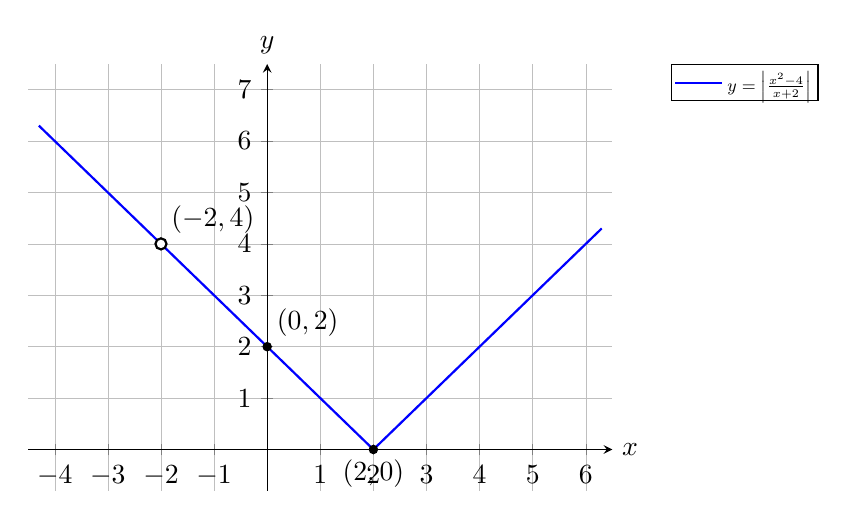
\begin{tikzpicture}
                \begin{axis}[
        axis lines = middle,
        xlabel = $x$,
        ylabel = {$y$},
        grid=both,
        grid style={line width=.1pt, draw=gray!10},
        major grid style={line width=.2pt,draw=gray!50},
        x label style={anchor=west}, % label x ke kanan
        y label style={anchor=south}, % label y ke atas
        samples=200,
        legend style={
                at={(1.1,1)},
                anchor=north west,
                font=\small,         % mengecilkan ukuran font
                row sep=1pt,         % jarak antar baris legend
                inner sep=1pt,       % margin dalam kotak legend
                nodes={scale=0.7}    % skalakan isi legend
            },
        xtick={-4,-3,...,6},
        ytick={0,1,...,7},
        xmin=-4.5, xmax=6.5,
        ymin=-0.8, ymax=7.5,
        width=9cm,
        height=7cm
    ]
\addplot[domain=-4.3:2, color=blue, thick, samples=2] {2-x};
\addlegendentry{$y=\left|\frac{x^2-4}{x+2}\right|$}
\addplot[domain=2:6.3, color=blue, thick, samples=2, forget plot] {x-2};
\draw[fill=white, thick] (-2,4) circle (2pt) node[above right] {$(-2,4)$};
\draw[fill=black] (2,0) circle (1.5pt) node[below] {$(2,0)$};
\draw[fill=black] (0,2) circle (1.5pt) node[above right] {$(0,2)$};
\end{axis}
            \end{tikzpicture}
        \end{center}
    }
    \end{jawab}

    \item \textbf{[Subbab 3.4]} Diberikan fungsi
    \begin{align*}
        f(x)=\begin{cases}
            \dfrac{x-16}{\sqrt{x}-4}, & x\neq 16\\
            7, & x=16
        \end{cases}.
    \end{align*}
    Selidiki kekontinuan $f(x)$ di $x=16$. Jika tidak kontinu, apakah diskontinuitasnya dapat dihilangkan? Jelaskan.
    \begin{jawab}[kekontinuan, limit fungsi, diskontinuitas yang dapat dihapus]{~\\
        Ingat kembali syarat fungsi kontinu di suatu titik \(x = a\) adalah
        \begin{enumerate}
            \item \(f(a)\) terdefinisi
            \item \(\displaystyle \lim_{x \to a} f(x)\) ada, yaitu $\displaystyle \lim_{x \to a^-} f(x) = \lim_{x \to a^+} f(x)$
            \item \(\displaystyle\lim_{x \to a} f(x) = f(a)\)
        \end{enumerate}
        Diperhatikan bahwa untuk $x=16$, $\colorlet{oldcolor}{.}
        \color{blue}
        \setlength{\fboxrule}{1pt} \boxed{\color{oldcolor}f(16) = 7~\text{terdefinisi}}\color{oldcolor}$. Selanjutnya, karena $x-16=(\sqrt{x})^2-4^2=(\sqrt{x}-4)(\sqrt{x}+4)$ untuk $x\geq 0$, limitnya adalah
        \begin{align*}
            \lim_{x\to 16} f(x) = \lim_{x\to 16} \frac{x-16}{\sqrt{x}-4} = \lim_{x\to 16} \frac{(\sqrt{x}-4)(\sqrt{x}+4)}{\sqrt{x}-4} = \lim_{x\to 16} (\sqrt{x}+4) = 4+4 = \colorlet{oldcolor}{.}
        \color{blue}
        \setlength{\fboxrule}{1pt} \boxed{\color{oldcolor}8}\color{oldcolor}.
        \end{align*}
        Syarat pertama dan kedua terpenuhi, tetapi $\displaystyle\lim_{x\to 16}f(x)=8\neq 7=f(16)$, sehingga syarat ketiga tidak terpenuhi. Jadi $\colorlet{oldcolor}{.}
        \color{red}
        \setlength{\fboxrule}{1pt} \boxed{\color{oldcolor}f \text{ tidak kontinu di } x=16}\color{oldcolor}$.\\
        Karena $\displaystyle\lim_{x\to 16}f(x)$ ada (bernilai $8$), maka diskontinuitas di $x=16$ $\colorlet{oldcolor}{.}
        \color{red}
        \setlength{\fboxrule}{1pt} \boxed{\color{oldcolor}\text{dapat dihilangkan}}\color{oldcolor}$, yaitu dengan mendefinisikan ulang nilai fungsi di titik tersebut menjadi $f(16)=8$. Dengan definisi baru ini, $f(x)=\sqrt{x}+4$ untuk setiap $x\geq 0$, dan $f$ kontinu di $x=16$.
    }
    \end{jawab}

    \item \textbf{[Subbab 4.3]} Dapatkan $f''(x)$ dimana $f(x)=\dfrac{x^2+1}{x-1}$.
    \begin{jawab}[turunan kedua, aturan pembagian]{~\\
        Ingat kembali aturan turunan untuk pembagian fungsi, yaitu
        \[
        \colorlet{oldcolor}{.}
        \color{blue}
        \setlength{\fboxrule}{1pt} \boxed{\color{oldcolor}\left(\frac{u}{v}\right)' = \frac{u'v - uv'}{v^2}}\color{oldcolor}.
        \]
        Misalkan $u=x^2+1$ dan $v=x-1$, maka $u'=2x$ dan $v'=1$. Turunan pertama dari $f$ adalah
        \begin{align*}
            f'(x) = \frac{2x(x-1)-(x^2+1)(1)}{(x-1)^2} = \frac{2x^2-2x-x^2-1}{(x-1)^2} = \colorlet{oldcolor}{.}
        \color{blue}
        \setlength{\fboxrule}{1pt} \boxed{\color{oldcolor}\frac{x^2-2x-1}{(x-1)^2}}\color{oldcolor}.
        \end{align*}
        Untuk turunan kedua, aturan pembagian digunakan sekali lagi dengan $u=x^2-2x-1$ dan $v=(x-1)^2=x^2-2x+1$, sehingga $u'=2x-2=2(x-1)$ dan $v'=2x-2=2(x-1)$. Diperoleh
        \begin{align*}
            f''(x) &= \frac{2(x-1)\cdot(x-1)^2-(x^2-2x-1)\cdot 2(x-1)}{(x-1)^4}\\
            &= \frac{2(x-1)\left[(x-1)^2-(x^2-2x-1)\right]}{(x-1)^4}\\
            &= \frac{2\left[x^2-2x+1-x^2+2x+1\right]}{(x-1)^3}\\
            &= \colorlet{oldcolor}{.}
        \color{red}
        \setlength{\fboxrule}{1pt} \boxed{\color{oldcolor}\frac{4}{(x-1)^3}}\color{oldcolor}, \quad x\neq 1.
        \end{align*}
    }
    \end{jawab}

\end{enumerate}

\newpage

%%%%%%%%%%%%%%%%%%%%%%%%%%%%%%%%%%%%%%%%%%%%%%%%%%%%%%%%%%%%%%%%%%%%%%%%%%%%%%
% Kal-1
% Kisi-kisi hari Selasa: subbab 1.2, 1.4, 2.1, 2.2, 3.2, 3.4, 4.2, 4.3
\kopsoal{Kal-1}{1-6}{Fisika, T. Kimia, T. Pangan}{Selasa, Kamis; 12.30-15.00}{8}
\begin{enumerate}
    \item \textbf{[Subbab 1.2]} Tentukan himpunan penyelesaian dari
    \begin{align*}
        \frac{5}{|3x-2|}\geq 2.
    \end{align*}
    \begin{jawab}[pertidaksamaan nilai mutlak, sifat nilai mutlak, notasi interval]{~\\
        Agar bentuk $\frac{5}{|3x-2|}$ terdefinisi, haruslah $\colorlet{oldcolor}{.}
        \color{blue}
        \setlength{\fboxrule}{1pt} \boxed{\color{oldcolor}x\neq\frac{2}{3}}\color{oldcolor}$, sehingga $|3x-2|>0$. Karena $|3x-2|$ positif, kedua ruas dapat dikalikan dengan $|3x-2|$ tanpa mengubah arah tanda pertidaksamaan, sehingga
        \begin{align*}
            \frac{5}{|3x-2|}\geq 2 \iff 5\geq 2|3x-2| \iff \colorlet{oldcolor}{.}
        \color{blue}
        \setlength{\fboxrule}{1pt} \boxed{\color{oldcolor}|3x-2|\leq\frac{5}{2}}\color{oldcolor}.
        \end{align*}
        Ingat kembali sifat nilai mutlak, yaitu untuk $a>0$ berlaku $\colorlet{oldcolor}{.}
        \color{blue}
        \setlength{\fboxrule}{1pt} \boxed{\color{oldcolor}|u|\leq a \iff -a\leq u\leq a}\color{oldcolor}$. Diperoleh
        \begin{align*}
            -\frac{5}{2}\leq 3x-2\leq\frac{5}{2} \iff -\frac{1}{2}\leq 3x\leq\frac{9}{2} \iff -\frac{1}{6}\leq x\leq\frac{3}{2}.
        \end{align*}
        Dengan mengingat syarat $x\neq\frac{2}{3}$, penyelesaiannya dapat digambarkan pada garis bilangan sebagai berikut
        \begin{center}
            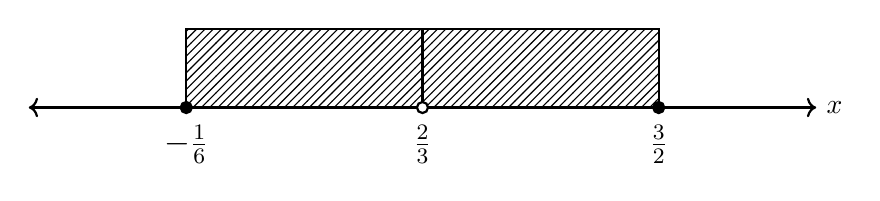
\begin{tikzpicture}
    \draw[thick,<->] (-5,0) -- (5,0) node[right] {$x$};
    \fill[pattern=north east lines] (-3,0) rectangle (3,1);
    \draw[thick] (-3,0) -- (-3,1) -- (3,1) -- (3,0);
    \draw (-3,-0.1) node[below] {\large{$-\frac{1}{6}$}};
    \draw (0,-0.1) node[below] {\large{$\frac{2}{3}$}};
    \draw (3,-0.1) node[below] {\large{$\frac{3}{2}$}};
    \draw[thick] (0,0) -- (0,1);
    \draw[fill=black, thick] (-3,0) circle (2pt);
    \draw[fill=white, thick] (0,0) circle (2pt);
    \draw[fill=black, thick] (3,0) circle (2pt);
            \end{tikzpicture}
        \end{center}
        Jadi himpunan penyelesaiannya adalah
        \[
        \colorlet{oldcolor}{.}
        \color{red}
        \setlength{\fboxrule}{1pt} \boxed{\color{oldcolor}\left[-\frac{1}{6},\frac{2}{3}\right)\cup\left(\frac{2}{3},\frac{3}{2}\right]}\color{oldcolor}.
        \]
    }
    \end{jawab}

    \item \textbf{[Subbab 2.1, 2.2]} Diberikan fungsi $f(x)=\dfrac{1}{x-3}$ dan $g(x)=\sqrt{7-x}$. Tentukan:
    \begin{enumerate}
        \item Domain fungsi $f$ dan $g$.
        \item Fungsi $(f\circ g)(x)$ dan $\left(\dfrac{f}{g}\right)(x)$ beserta domainnya masing-masing.
    \end{enumerate}
    \begin{jawab}[domain fungsi, fungsi komposisi, operasi pembagian fungsi, domain fungsi]{
        \begin{enumerate}
            \item Diperhatikan bahwa $f(x)$ merupakan fungsi rasional, sehingga domainnya adalah semua bilangan real kecuali nilai yang membuat penyebutnya sama dengan nol, yaitu $x-3\neq 0$. Jadi
            \[
            \colorlet{oldcolor}{.}
        \color{red}
        \setlength{\fboxrule}{1pt} \boxed{\color{oldcolor}D(f)=\{x \in \mathbb{R} : x \neq 3\}}\color{oldcolor}.
            \]
            Selanjutnya, diperhatikan bahwa $g(x)$ memuat akar kuadrat, sehingga domainnya adalah semua bilangan real yang membuat ekspresi di dalam akar kuadrat tak negatif, yaitu $7-x\geq 0$. Jadi
            \[
            \colorlet{oldcolor}{.}
        \color{red}
        \setlength{\fboxrule}{1pt} \boxed{\color{oldcolor}D(g)=\{x \in \mathbb{R} : x \leq 7\}=(-\infty,7]}\color{oldcolor}.
            \]
            \item Diperhatikan bahwa
            \begin{align*}
                (f\circ g)(x) = f(g(x)) = f\left(\sqrt{7-x}\right) = \colorlet{oldcolor}{.}
        \color{red}
        \setlength{\fboxrule}{1pt} \boxed{\color{oldcolor}\frac{1}{\sqrt{7-x} - 3}}\color{oldcolor}
            \end{align*}
            Domain dari fungsi komposisi $f\circ g$ adalah semua nilai $x$ pada domain $g$ sehingga nilai dari $g(x)$ berada pada domain $f$, yang dapat dirumuskan sebagai
            \begin{align*}
                \colorlet{oldcolor}{.}
        \color{blue}
        \setlength{\fboxrule}{1pt} \boxed{\color{oldcolor}D(f\circ g) = \{x \in D(g) : g(x) \in D(f)\} = \left\{x \in (-\infty, 7] : \sqrt{7-x} \neq 3\right\}}\color{oldcolor}.
            \end{align*}
            Karena $\sqrt{7-x} = 3$ jika dan hanya jika $7-x = 9$, yang berarti $x = -2$, didapatkan
            \begin{align*}
                \colorlet{oldcolor}{.}
        \color{red}
        \setlength{\fboxrule}{1pt} \boxed{\color{oldcolor}D(f\circ g) = (-\infty, 7] \setminus \{-2\} = (-\infty, -2) \cup (-2, 7]}\color{oldcolor}.
            \end{align*}
            Selanjutnya, untuk pembagian fungsi diperoleh
            \begin{align*}
                \left(\frac{f}{g}\right)(x) = \frac{f(x)}{g(x)} = \frac{\frac{1}{x-3}}{\sqrt{7-x}} = \colorlet{oldcolor}{.}
        \color{red}
        \setlength{\fboxrule}{1pt} \boxed{\color{oldcolor}\frac{1}{(x-3)\sqrt{7-x}}}\color{oldcolor}.
            \end{align*}
            Domain dari $\frac{f}{g}$ adalah irisan domain $f$ dan $g$, dikurangi nilai $x$ yang membuat $g(x)=0$, yaitu
            \begin{align*}
                \colorlet{oldcolor}{.}
        \color{blue}
        \setlength{\fboxrule}{1pt} \boxed{\color{oldcolor}D\left(\frac{f}{g}\right) = \{x \in D(f)\cap D(g) : g(x) \neq 0\}}\color{oldcolor}.
            \end{align*}
            Karena $D(f)\cap D(g) = (-\infty,3)\cup(3,7]$ dan $g(x)=\sqrt{7-x}=0$ jika dan hanya jika $x=7$, didapatkan
            \begin{align*}
                \colorlet{oldcolor}{.}
        \color{red}
        \setlength{\fboxrule}{1pt} \boxed{\color{oldcolor}D\left(\frac{f}{g}\right) = (-\infty, 3) \cup (3, 7)}\color{oldcolor}.
            \end{align*}
        \end{enumerate}
    }
    \end{jawab}

    \item \textbf{[Subbab 1.4]} Diberikan titik $A(-1,-3)$, $B(1,1)$, dan $C(5,2)$. Garis $\ell$ melalui titik $A$ dan $B$.
    \begin{enumerate}
        \item Dapatkan jarak titik $C$ ke garis $\ell$.
        \item Dapatkan persamaan garis yang melalui $C$ dan sejajar dengan garis $\ell$.
    \end{enumerate}
    \begin{jawab}[gradien garis, persamaan garis, jarak titik ke garis, garis sejajar]{
        \begin{enumerate}
            \item Terlebih dahulu ditentukan persamaan garis $\ell$. Gradien garis yang melalui $A(-1,-3)$ dan $B(1,1)$ adalah
            \begin{align*}
                m_\ell = \frac{1-(-3)}{1-(-1)} = \frac{4}{2} = \colorlet{oldcolor}{.}
        \color{blue}
        \setlength{\fboxrule}{1pt} \boxed{\color{oldcolor}2}\color{oldcolor}.
            \end{align*}
            Karena $\ell$ melalui $B(1,1)$, persamaannya adalah
            \begin{align*}
                y-1=2(x-1) \iff y=2x-1 \iff \colorlet{oldcolor}{.}
        \color{blue}
        \setlength{\fboxrule}{1pt} \boxed{\color{oldcolor}2x-y-1=0}\color{oldcolor}.
            \end{align*}
            Ingat kembali rumus jarak titik $(x_0,y_0)$ ke garis $ax+by+c=0$, yaitu
            \begin{align*}
                \colorlet{oldcolor}{.}
        \color{blue}
        \setlength{\fboxrule}{1pt} \boxed{\color{oldcolor}d = \frac{|ax_0+by_0+c|}{\sqrt{a^2+b^2}}}\color{oldcolor}.
            \end{align*}
            Dengan $a=2$, $b=-1$, $c=-1$, dan titik $C(5,2)$, diperoleh
            \begin{align*}
                d = \frac{|2(5)-2-1|}{\sqrt{2^2+(-1)^2}} = \frac{7}{\sqrt{5}} = \colorlet{oldcolor}{.}
        \color{red}
        \setlength{\fboxrule}{1pt} \boxed{\color{oldcolor}\frac{7}{5}\sqrt{5}}\color{oldcolor}.
            \end{align*}
            \item Dua garis sejajar memiliki gradien yang sama, sehingga garis yang dicari memiliki gradien $2$ dan melalui $C(5,2)$. Dengan rumus $y - y_1 = m(x - x_1)$, diperoleh
            \begin{align*}
                y - 2 = 2(x - 5) \implies y = 2x - 8.
            \end{align*}
            Jadi persamaan garisnya adalah $\colorlet{oldcolor}{.}
        \color{red}
        \setlength{\fboxrule}{1pt} \boxed{\color{oldcolor}y = 2x - 8}\color{oldcolor}$ atau $2x-y-8=0$.
        \end{enumerate}
    }
    \end{jawab}

    \item \textbf{[Subbab 3.4]} Diberikan fungsi
    \begin{align*}
        f(x)=\begin{cases}
            \dfrac{9-x}{3-\sqrt{x}}, & x\neq 9\\
            k, & x=9
        \end{cases},\quad \text{dengan } x\in[0,\infty).
    \end{align*}
    \begin{enumerate}
        \item Tentukan nilai $k$ sehingga $f(x)$ kontinu di $x=9$.
        \item Untuk nilai $k$ tersebut, nyatakan $f(x)$ tanpa menggunakan bentuk fungsi sepotong-sepotong.
    \end{enumerate}
    \begin{jawab}[fungsi kontinu, limit fungsi, fungsi sepotong-sepotong]{
        \begin{enumerate}
            \item Ingat kembali syarat fungsi kontinu di suatu titik \(x = a\) adalah
            \begin{enumerate}
                \item \(f(a)\) terdefinisi
                \item \(\displaystyle \lim_{x \to a} f(x)\) ada, yaitu $\displaystyle \lim_{x \to a^-} f(x) = \lim_{x \to a^+} f(x)$
                \item \(\displaystyle\lim_{x \to a} f(x) = f(a)\)
            \end{enumerate}
            Diperhatikan bahwa untuk \(x = 9\), \(\colorlet{oldcolor}{.}
        \color{blue}
        \setlength{\fboxrule}{1pt} \boxed{\color{oldcolor}f(9) = k~\text{terdefinisi}}\color{oldcolor}\). Karena untuk $x\geq 0$ berlaku $9-x=3^2-(\sqrt{x})^2=(3-\sqrt{x})(3+\sqrt{x})$, didapatkan limitnya adalah
            \begin{align*}
            \lim_{x \to 9} f(x) = \lim_{x \to 9} \frac{9-x}{3-\sqrt{x}} = \lim_{x \to 9} \frac{(3-\sqrt{x})(3+\sqrt{x})}{3-\sqrt{x}} = \lim_{x \to 9} (3+\sqrt{x}) = 3+3 = \colorlet{oldcolor}{.}
        \color{blue}
        \setlength{\fboxrule}{1pt} \boxed{\color{oldcolor}6}\color{oldcolor}.
            \end{align*}
            Selanjutnya, untuk syarat ketiga, haruslah $\displaystyle \colorlet{oldcolor}{.}
        \color{blue}
        \setlength{\fboxrule}{1pt} \boxed{\color{oldcolor}\lim_{x \to 9} f(x) = f(9)}\color{oldcolor}$, sehingga diperoleh $\colorlet{oldcolor}{.}
        \color{red}
        \setlength{\fboxrule}{1pt} \boxed{\color{oldcolor}k=6}\color{oldcolor}$.
            \item Diperhatikan bahwa untuk $x\in[0,\infty)$ dengan $x\neq 9$ berlaku $f(x)=3+\sqrt{x}$ (dari proses perhitungan limit di atas), dan untuk $x=9$ nilai $3+\sqrt{9}=6=k=f(9)$. Dengan demikian, fungsi $f(x)$ dapat dinyatakan tanpa bentuk sepotong-sepotong sebagai
            \begin{align*}
                \colorlet{oldcolor}{.}
        \color{red}
        \setlength{\fboxrule}{1pt} \boxed{\color{oldcolor}f(x) = 3+\sqrt{x}, \quad x \in [0,\infty)}\color{oldcolor}.
            \end{align*}
        \end{enumerate}
    }
    \end{jawab}

    \item \textbf{[Subbab 4.3]} Dapatkan $f''(x)$ dimana $f(x)=x^3+\dfrac{x}{x+1}$.
    \begin{jawab}[turunan kedua, aturan pembagian]{~\\
        Ingat kembali aturan turunan untuk pembagian fungsi, yaitu
        \[
        \colorlet{oldcolor}{.}
        \color{blue}
        \setlength{\fboxrule}{1pt} \boxed{\color{oldcolor}\left(\frac{u}{v}\right)' = \frac{u'v - uv'}{v^2}}\color{oldcolor}.
        \]
        Untuk suku $\frac{x}{x+1}$, misalkan $u=x$ dan $v=x+1$, maka $u'=1$ dan $v'=1$, sehingga
        \begin{align*}
            \frac{d}{dx}\left(\frac{x}{x+1}\right) = \frac{1\cdot(x+1)-x\cdot 1}{(x+1)^2} = \frac{1}{(x+1)^2}.
        \end{align*}
        Dengan demikian, turunan pertama dari $f$ adalah
        \begin{align*}
            \colorlet{oldcolor}{.}
        \color{blue}
        \setlength{\fboxrule}{1pt} \boxed{\color{oldcolor}f'(x) = 3x^2+\frac{1}{(x+1)^2}}\color{oldcolor}.
        \end{align*}
        Untuk turunan kedua, suku $\frac{1}{(x+1)^2}=\frac{1}{x^2+2x+1}$ diturunkan dengan aturan pembagian, dengan $u=1$ dan $v=x^2+2x+1$, sehingga $u'=0$ dan $v'=2x+2=2(x+1)$. Diperoleh
        \begin{align*}
            \frac{d}{dx}\left(\frac{1}{(x+1)^2}\right) = \frac{0\cdot(x+1)^2-1\cdot 2(x+1)}{(x+1)^4} = -\frac{2}{(x+1)^3}.
        \end{align*}
        Jadi turunan kedua dari $f$ adalah
        \begin{align*}
            f''(x) = \colorlet{oldcolor}{.}
        \color{red}
        \setlength{\fboxrule}{1pt} \boxed{\color{oldcolor}6x-\frac{2}{(x+1)^3}}\color{oldcolor}, \quad x\neq -1.
        \end{align*}
    }
    \end{jawab}

\end{enumerate}

\newpage

%%%%%%%%%%%%%%%%%%%%%%%%%%%%%%%%%%%%%%%%%%%%%%%%%%%%%%%%%%%%%%%%%%%%%%%%%%%%%%
% Kal-2
% Kisi-kisi hari Selasa: subbab 1.2, 1.4, 2.1, 2.2, 3.2, 3.4, 4.2, 4.3
\kopsoal{Kal-2}{7-12}{T. Lingkungan, T. Elektro, T. Biomedik}{Selasa, Kamis; 12.30-15.00}{8}
\begin{enumerate}
    \item \textbf{[Subbab 1.4]} Diberikan garis $\ell$ melalui titik $(3,2)$ dan $(a,b)$ dengan kemiringan $2$, dan garis $k$ melalui titik $(0,-1)$ dan $(a,b)$ dengan kemiringan $-1$. Dapatkan nilai $a$ dan $b$.
    \begin{jawab}[kemiringan garis, persamaan garis, sistem persamaan linear]{~\\
        Kemiringan garis yang melalui dua titik $(x_1,y_1)$ dan $(x_2,y_2)$ adalah $\colorlet{oldcolor}{.}
        \color{blue}
        \setlength{\fboxrule}{1pt} \boxed{\color{oldcolor}m = \frac{y_2 - y_1}{x_2 - x_1}}\color{oldcolor}$.
        \begin{itemize}
            \item Garis $\ell$ melalui $(3,2)$ dan $(a,b)$ dengan kemiringan $2$, sehingga
            \begin{align*}
                \frac{b-2}{a-3} = 2 \implies b-2 = 2a-6 \implies \colorlet{oldcolor}{.}
        \color{blue}
        \setlength{\fboxrule}{1pt} \boxed{\color{oldcolor}b = 2a-4}\color{oldcolor}.
            \end{align*}
            \item Garis $k$ melalui $(0,-1)$ dan $(a,b)$ dengan kemiringan $-1$, sehingga
            \begin{align*}
                \frac{b-(-1)}{a-0} = -1 \implies b+1 = -a \implies \colorlet{oldcolor}{.}
        \color{blue}
        \setlength{\fboxrule}{1pt} \boxed{\color{oldcolor}b = -a-1}\color{oldcolor}.
            \end{align*}
        \end{itemize}
        Dengan menyamakan kedua persamaan tersebut, diperoleh
        \begin{align*}
            2a-4 = -a-1 \implies 3a = 3 \implies a = 1,
        \end{align*}
        dan $b=2(1)-4=-2$. Sebagai pengecekan, kemiringan dari $(3,2)$ ke $(1,-2)$ adalah $\frac{-2-2}{1-3}=2$, dan kemiringan dari $(0,-1)$ ke $(1,-2)$ adalah $\frac{-2+1}{1-0}=-1$. Jadi $\colorlet{oldcolor}{.}
        \color{red}
        \setlength{\fboxrule}{1pt} \boxed{\color{oldcolor}a=1 \text{ dan } b=-2}\color{oldcolor}$, yaitu titik $(a,b)=(1,-2)$ merupakan titik potong kedua garis.
    }
    \end{jawab}

    \item \textbf{[Subbab 1.2]} Tentukan semua nilai $x$ yang memenuhi pertidaksamaan
    \begin{align*}
        |x+4|\leq|2x-1|.
    \end{align*}
    \begin{jawab}[pertidaksamaan nilai mutlak, sifat nilai mutlak, pertidaksamaan kuadrat]{~\\
        Karena kedua ruas bernilai tak negatif, kedua ruas dapat dikuadratkan tanpa mengubah arah tanda pertidaksamaan. Ingat kembali bahwa $\colorlet{oldcolor}{.}
        \color{blue}
        \setlength{\fboxrule}{1pt} \boxed{\color{oldcolor}|u|\leq|v| \iff u^2\leq v^2}\color{oldcolor}$. Diperoleh
        \begin{align*}
            (x+4)^2 &\leq (2x-1)^2\\
            x^2+8x+16 &\leq 4x^2-4x+1\\
            0 &\leq 3x^2-12x-15\\
            0 &\leq 3(x-5)(x+1).
        \end{align*}
        Pembuat nolnya adalah $\colorlet{oldcolor}{.}
        \color{blue}
        \setlength{\fboxrule}{1pt} \boxed{\color{oldcolor}x=-1}\color{oldcolor}$ dan $\colorlet{oldcolor}{.}
        \color{blue}
        \setlength{\fboxrule}{1pt} \boxed{\color{oldcolor}x=5}\color{oldcolor}$. Dengan uji titik, misalkan $x=-2$ diperoleh $3(-7)(-1)>0$, $x=0$ diperoleh $3(-5)(1)<0$, dan $x=6$ diperoleh $3(1)(7)>0$.
        \begin{center}
            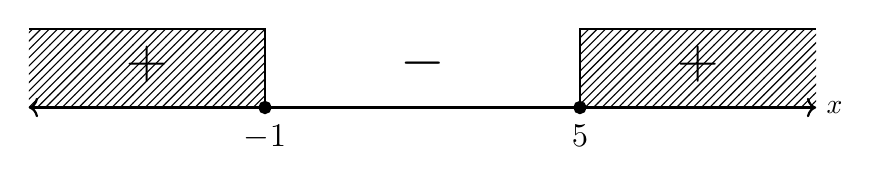
\begin{tikzpicture}
    \draw[thick,<->] (-5,0) -- (5,0) node[right] {$x$};
    \fill[pattern=north east lines] (-5,0) rectangle (-2,1);
    \fill[pattern=north east lines] (2,0) rectangle (5,1);
    \draw[thick] (-5,1) -- (-2,1) -- (-2,0);
    \draw[thick] (2,0) -- (2,1) -- (5,1);
    \draw (-2,-0.1) node[below] {\large{$-1$}};
    \draw (2,-0.1) node[below] {\large{$5$}};
    \draw (-3.5,0.2) node[above] {\huge{$+$}};
    \draw (0,0.2) node[above] {\huge{$-$}};
    \draw (3.5,0.2) node[above] {\huge{$+$}};
    \draw[fill=black, thick] (-2,0) circle (2pt);
    \draw[fill=black, thick] (2,0) circle (2pt);
            \end{tikzpicture}
        \end{center}
        Sebagai pengecekan, untuk $x=6$ diperoleh $|10|=10\leq|11|=11$, sedangkan untuk $x=0$ diperoleh $|4|=4\not\leq|-1|=1$. Jadi semua nilai $x$ yang memenuhi adalah $x\leq -1$ atau $x\geq 5$, atau dalam notasi interval $\colorlet{oldcolor}{.}
        \color{red}
        \setlength{\fboxrule}{1pt} \boxed{\color{oldcolor}(-\infty,-1]\cup[5,\infty)}\color{oldcolor}$.
    }
    \end{jawab}

    \item \textbf{[Subbab 2.1, 2.2]} Diberikan fungsi $f(x)=\sqrt{x^2-4}$ dan $g(x)=\dfrac{4}{x}$.
    \begin{enumerate}
        \item Dapatkan domain $f$ dan $g$.
        \item Dapatkan fungsi $(f\cdot g)(x)$ beserta domainnya.
        \item Dapatkan fungsi $f(g(x))$ beserta domainnya.
    \end{enumerate}
    \begin{jawab}[domain fungsi, operasi perkalian fungsi, fungsi komposisi, domain fungsi komposisi]{
        \begin{enumerate}
            \item Fungsi $f$ terdefinisi jika $x^2-4\geq 0$, yaitu $(x-2)(x+2)\geq 0$, yang dipenuhi oleh $x\leq -2$ atau $x\geq 2$. Fungsi $g$ terdefinisi jika $x\neq 0$. Jadi
            \begin{align*}
                \colorlet{oldcolor}{.}
        \color{red}
        \setlength{\fboxrule}{1pt} \boxed{\color{oldcolor}D(f)=(-\infty,-2]\cup[2,\infty)}\color{oldcolor} \quad\text{dan}\quad \colorlet{oldcolor}{.}
        \color{red}
        \setlength{\fboxrule}{1pt} \boxed{\color{oldcolor}D(g)=\mathbb{R}\setminus\{0\}}\color{oldcolor}.
            \end{align*}
            \item Diperoleh $(f\cdot g)(x)=f(x)\cdot g(x)=\sqrt{x^2-4}\cdot\frac{4}{x}=\colorlet{oldcolor}{.}
        \color{red}
        \setlength{\fboxrule}{1pt} \boxed{\color{oldcolor}\frac{4\sqrt{x^2-4}}{x}}\color{oldcolor}$. Domain dari $f\cdot g$ adalah irisan domain $f$ dan $g$, yaitu
            \begin{align*}
                \colorlet{oldcolor}{.}
        \color{blue}
        \setlength{\fboxrule}{1pt} \boxed{\color{oldcolor}D(f\cdot g)=D(f)\cap D(g)}\color{oldcolor} = \colorlet{oldcolor}{.}
        \color{red}
        \setlength{\fboxrule}{1pt} \boxed{\color{oldcolor}(-\infty,-2]\cup[2,\infty)}\color{oldcolor},
            \end{align*}
            karena $x=0$ memang tidak termasuk dalam $D(f)$.
            \item Diperhatikan bahwa
            \begin{align*}
                f(g(x)) = f\left(\frac{4}{x}\right) = \sqrt{\frac{16}{x^2}-4} = \sqrt{\frac{16-4x^2}{x^2}} = \colorlet{oldcolor}{.}
        \color{red}
        \setlength{\fboxrule}{1pt} \boxed{\color{oldcolor}\frac{2\sqrt{4-x^2}}{|x|}}\color{oldcolor}.
            \end{align*}
            Domain dari fungsi komposisi adalah semua nilai $x$ pada domain $g$ sehingga nilai dari $g(x)$ berada pada domain $f$, yaitu
            \begin{align*}
                \colorlet{oldcolor}{.}
        \color{blue}
        \setlength{\fboxrule}{1pt} \boxed{\color{oldcolor}D(f\circ g) = \{x \in D(g) : g(x) \in D(f)\} = \left\{x\neq 0 : \frac{16}{x^2}-4\geq 0\right\}}\color{oldcolor}.
            \end{align*}
            Untuk $x\neq 0$, syarat $\frac{16}{x^2}\geq 4$ setara dengan $x^2\leq 4$, yaitu $-2\leq x\leq 2$. Dengan mengecualikan $x=0$, didapatkan
            \begin{align*}
                \colorlet{oldcolor}{.}
        \color{red}
        \setlength{\fboxrule}{1pt} \boxed{\color{oldcolor}D(f\circ g) = [-2,0)\cup(0,2]}\color{oldcolor}.
            \end{align*}
        \end{enumerate}
    }
    \end{jawab}

    \item \textbf{[Subbab 3.4]} Diberikan fungsi
    \begin{align*}
        f(x)=\begin{cases}
            ax+b, & x<1\\
            x^2+2x, & x\geq 1
        \end{cases}.
    \end{align*}
    Tentukan nilai $a$ dan $b$ agar $f$ kontinu di $x=1$ dan $f(-1)=-1$.
    \begin{jawab}[kekontinuan, limit sepihak, sistem persamaan linear]{~\\
        Ingat kembali syarat fungsi kontinu di suatu titik \(x = c\) adalah
        \begin{enumerate}
            \item \(f(c)\) terdefinisi
            \item \(\displaystyle \lim_{x \to c} f(x)\) ada, yaitu $\displaystyle \lim_{x \to c^-} f(x) = \lim_{x \to c^+} f(x)$
            \item \(\displaystyle\lim_{x \to c} f(x) = f(c)\)
        \end{enumerate}
        Diperhatikan bahwa $\colorlet{oldcolor}{.}
        \color{blue}
        \setlength{\fboxrule}{1pt} \boxed{\color{oldcolor}f(1)=1^2+2(1)=3~\text{terdefinisi}}\color{oldcolor}$, serta
        \begin{align*}
            \lim_{x\to 1^-}f(x)=\lim_{x\to 1^-}(ax+b)=a+b \quad\text{dan}\quad \lim_{x\to 1^+}f(x)=\lim_{x\to 1^+}(x^2+2x)=3.
        \end{align*}
        Agar $f$ kontinu di $x=1$, haruslah $\colorlet{oldcolor}{.}
        \color{blue}
        \setlength{\fboxrule}{1pt} \boxed{\color{oldcolor}a+b=3}\color{oldcolor}$. Selanjutnya, karena $-1<1$, nilai $f(-1)$ dihitung dengan rumus $ax+b$, sehingga syarat $f(-1)=-1$ memberikan $\colorlet{oldcolor}{.}
        \color{blue}
        \setlength{\fboxrule}{1pt} \boxed{\color{oldcolor}-a+b=-1}\color{oldcolor}$. Dengan menjumlahkan kedua persamaan, diperoleh $2b=2$, yaitu $b=1$, dan $a=3-1=2$.\\
        Sebagai pengecekan, untuk $a=2$ dan $b=1$ diperoleh $f(x)=2x+1$ untuk $x<1$, sehingga $\displaystyle\lim_{x\to 1^-}f(x)=3=f(1)$ dan $f(-1)=-2+1=-1$. Jadi $\colorlet{oldcolor}{.}
        \color{red}
        \setlength{\fboxrule}{1pt} \boxed{\color{oldcolor}a=2 \text{ dan } b=1}\color{oldcolor}$.
    }
    \end{jawab}

    \item \textbf{[Subbab 4.3]} Diberikan kurva $y=\dfrac{x+5}{x+3}$. Dapatkan titik-titik pada kurva yang garis singgungnya sejajar dengan garis $y=-2x+1$, beserta persamaan garis singgungnya.
    \begin{jawab}[turunan, aturan pembagian, garis sejajar, persamaan garis singgung]{~\\
        Ingat kembali aturan turunan untuk pembagian fungsi, yaitu $\colorlet{oldcolor}{.}
        \color{blue}
        \setlength{\fboxrule}{1pt} \boxed{\color{oldcolor}\left(\frac{u}{v}\right)' = \frac{u'v - uv'}{v^2}}\color{oldcolor}$. Untuk $u=x+5$ dan $v=x+3$, diperoleh
        \begin{align*}
            y' = \frac{(1)(x+3)-(x+5)(1)}{(x+3)^2} = \colorlet{oldcolor}{.}
        \color{blue}
        \setlength{\fboxrule}{1pt} \boxed{\color{oldcolor}-\frac{2}{(x+3)^2}}\color{oldcolor}.
        \end{align*}
        Garis $y=-2x+1$ bergradien $-2$, sehingga garis singgung yang sejajar dengannya juga bergradien $-2$. Haruslah
        \begin{align*}
            -\frac{2}{(x+3)^2} = -2 \iff (x+3)^2=1 \iff x+3=\pm 1 \iff x=-2 \;\vee\; x=-4.
        \end{align*}
        Untuk $x=-2$ diperoleh $y=\frac{3}{1}=3$, dan untuk $x=-4$ diperoleh $y=\frac{1}{-1}=-1$. Dengan rumus $y - y_1 = m(x - x_1)$ dan $m=-2$, diperoleh
        \begin{itemize}
            \item di titik $(-2,3)$: $y-3=-2(x+2)$, yaitu $y=-2x-1$;
            \item di titik $(-4,-1)$: $y+1=-2(x+4)$, yaitu $y=-2x-9$.
        \end{itemize}
        Jadi titik-titiknya adalah $\colorlet{oldcolor}{.}
        \color{red}
        \setlength{\fboxrule}{1pt} \boxed{\color{oldcolor}(-2,3) \text{ dan } (-4,-1)}\color{oldcolor}$, dengan persamaan garis singgung
        \[\colorlet{oldcolor}{.}
        \color{red}
        \setlength{\fboxrule}{1pt} \boxed{\color{oldcolor}y=-2x-1 \quad\text{dan}\quad y=-2x-9}\color{oldcolor}.\]
    }
    \end{jawab}

\end{enumerate}

\newpage

%%%%%%%%%%%%%%%%%%%%%%%%%%%%%%%%%%%%%%%%%%%%%%%%%%%%%%%%%%%%%%%%%%%%%%%%%%%%%%
% Kal-10
% Kisi-kisi hari Selasa: subbab 1.2, 1.4, 2.1, 2.2, 3.2, 3.4, 4.2, 4.3
\kopsoal{Kal-10}{49-50}{Teknologi Kedokteran}{Selasa, Kamis; 12.30-15.00}{8}
\begin{enumerate}
    \item \textbf{[Subbab 1.2]} \begin{enumerate}
        \item Tuliskan kembali $|x|+2|x-2|$ tanpa menggunakan tanda nilai mutlak.
        \item Berdasarkan point (a), tentukan himpunan penyelesaian dari $|x|+2|x-2|\leq 5$.
    \end{enumerate}
    \begin{jawab}[definisi nilai mutlak, fungsi sepotong-sepotong, pertidaksamaan nilai mutlak]{
        \begin{enumerate}
            \item Ingat kembali definisi nilai mutlak, yaitu $|x|=x$ untuk $x\geq 0$ dan $|x|=-x$ untuk $x<0$, serta $|x-2|=x-2$ untuk $x\geq 2$ dan $|x-2|=-(x-2)$ untuk $x<2$. Titik-titik batasnya adalah $x=0$ dan $x=2$, sehingga
            \begin{itemize}
                \item untuk $x<0$: $|x|+2|x-2|=-x+2(2-x)=-3x+4$,
                \item untuk $0\leq x<2$: $|x|+2|x-2|=x+2(2-x)=-x+4$,
                \item untuk $x\geq 2$: $|x|+2|x-2|=x+2(x-2)=3x-4$.
            \end{itemize}
            Jadi
            \begin{align*}
                \colorlet{oldcolor}{.}
        \color{red}
        \setlength{\fboxrule}{1pt} \boxed{\color{oldcolor}|x|+2|x-2|=\begin{cases}
                    -3x+4, & x<0\\
                    -x+4, & 0\leq x<2\\
                    3x-4, & x\geq 2
                \end{cases}}\color{oldcolor}.
            \end{align*}
            \item Berdasarkan (a), pertidaksamaan $|x|+2|x-2|\leq 5$ diselesaikan pada setiap kasus.
            \begin{enumerate}
                \item[(i)] Jika $x<0$: $-3x+4\leq 5\iff x\geq -\frac{1}{3}$. Irisan dengan $x<0$ adalah $\colorlet{oldcolor}{.}
        \color{blue}
        \setlength{\fboxrule}{1pt} \boxed{\color{oldcolor}-\frac{1}{3}\leq x<0}\color{oldcolor}$.
                \item[(ii)] Jika $0\leq x<2$: $-x+4\leq 5\iff x\geq -1$. Irisan dengan $0\leq x<2$ adalah $\colorlet{oldcolor}{.}
        \color{blue}
        \setlength{\fboxrule}{1pt} \boxed{\color{oldcolor}0\leq x<2}\color{oldcolor}$.
                \item[(iii)] Jika $x\geq 2$: $3x-4\leq 5\iff x\leq 3$. Irisan dengan $x\geq 2$ adalah $\colorlet{oldcolor}{.}
        \color{blue}
        \setlength{\fboxrule}{1pt} \boxed{\color{oldcolor}2\leq x\leq 3}\color{oldcolor}$.
            \end{enumerate}
            Dengan menggabungkan ketiga kasus, diperoleh himpunan penyelesaian $\colorlet{oldcolor}{.}
        \color{red}
        \setlength{\fboxrule}{1pt} \boxed{\color{oldcolor}\left[-\frac{1}{3},3\right]}\color{oldcolor}$.
        \end{enumerate}
    }
    \end{jawab}

    \item \textbf{[Subbab 2.1, 2.2]} Diberikan fungsi $f(x)=\sqrt{2-x}$ dan $g(x)=\dfrac{1}{\sqrt{16-x^2}}$.
    \begin{enumerate}
        \item Dapatkan domain $f$ dan $g$.
        \item Dapatkan $(g\circ f)(x)$ beserta domainnya.
    \end{enumerate}
    \begin{jawab}[domain fungsi, fungsi komposisi, domain fungsi komposisi]{
        \begin{enumerate}
            \item Diperhatikan bahwa $f(x)$ memuat akar kuadrat, sehingga syaratnya adalah $2-x\geq 0$, yaitu $x\leq 2$. Jadi
            \begin{align*}
                \colorlet{oldcolor}{.}
        \color{red}
        \setlength{\fboxrule}{1pt} \boxed{\color{oldcolor}D(f)=\{x\in\mathbb{R} : x\leq 2\}=(-\infty,2]}\color{oldcolor}.
            \end{align*}
            Selanjutnya, $g(x)$ memuat akar kuadrat di penyebut, sehingga ekspresi di dalam akar harus positif (tidak boleh nol), yaitu $16-x^2>0$ atau $(4-x)(4+x)>0$, yang dipenuhi oleh $-4<x<4$. Jadi
            \begin{align*}
                \colorlet{oldcolor}{.}
        \color{red}
        \setlength{\fboxrule}{1pt} \boxed{\color{oldcolor}D(g)=\{x\in\mathbb{R} : -4<x<4\}=(-4,4)}\color{oldcolor}.
            \end{align*}
            \item Diperhatikan bahwa
            \begin{align*}
                (g\circ f)(x) = g(f(x)) = \frac{1}{\sqrt{16-\left(\sqrt{2-x}\right)^2}} = \frac{1}{\sqrt{16-(2-x)}} = \colorlet{oldcolor}{.}
        \color{red}
        \setlength{\fboxrule}{1pt} \boxed{\color{oldcolor}\frac{1}{\sqrt{14+x}}}\color{oldcolor}.
            \end{align*}
            Domain dari fungsi komposisi $g\circ f$ adalah semua nilai $x$ pada domain $f$ sehingga nilai dari $f(x)$ berada pada domain $g$, yang dapat dirumuskan sebagai
            \begin{align*}
                \colorlet{oldcolor}{.}
        \color{blue}
        \setlength{\fboxrule}{1pt} \boxed{\color{oldcolor}D(g\circ f) = \{x \in D(f) : f(x) \in D(g)\} = \left\{x \leq 2 : -4<\sqrt{2-x}<4\right\}}\color{oldcolor}.
            \end{align*}
            Karena $\sqrt{2-x}\geq 0>-4$, syarat $\sqrt{2-x}>-4$ selalu berlaku. Selanjutnya, $\sqrt{2-x}<4$ jika dan hanya jika $2-x<16$, yaitu $x>-14$. Dengan menggabungkan syarat $x\leq 2$, didapatkan
            \begin{align*}
                \colorlet{oldcolor}{.}
        \color{red}
        \setlength{\fboxrule}{1pt} \boxed{\color{oldcolor}D(g\circ f) = \{x\in\mathbb{R} : -14<x\leq 2\} = (-14,2]}\color{oldcolor}.
            \end{align*}
            \textit{Catatan:} meskipun bentuk akhir $\frac{1}{\sqrt{14+x}}$ terdefinisi untuk $x>2$, nilai-nilai tersebut tidak termasuk domain karena $f(x)$ tidak terdefinisi di sana.
        \end{enumerate}
    }
    \end{jawab}

    \item \textbf{[Subbab 1.4]} \begin{enumerate}
        \item Jika titik tengah antara titik $A(-1,2)$ dan titik $B$ adalah titik $C(1,3)$, tentukan koordinat titik $B$ dan panjang ruas garis $AB$.
        \item Dapatkan persamaan garis yang melalui $C$ dan tegak lurus dengan garis $AB$, kemudian tentukan jarak titik $A$ ke garis tersebut.
    \end{enumerate}
    \begin{jawab}[titik tengah, jarak dua titik, garis tegak lurus, jarak titik ke garis]{
        \begin{enumerate}
            \item Misalkan $B(x_B,y_B)$. Titik tengah dari dua titik $(x_1,y_1)$ dan $(x_2,y_2)$ adalah $\colorlet{oldcolor}{.}
        \color{blue}
        \setlength{\fboxrule}{1pt} \boxed{\color{oldcolor}\left(\frac{x_1+x_2}{2},\frac{y_1+y_2}{2}\right)}\color{oldcolor}$, sehingga
            \begin{align*}
                \frac{-1+x_B}{2}=1 \implies x_B=3 \quad\text{dan}\quad \frac{2+y_B}{2}=3 \implies y_B=4.
            \end{align*}
            Jadi $\colorlet{oldcolor}{.}
        \color{red}
        \setlength{\fboxrule}{1pt} \boxed{\color{oldcolor}B(3,4)}\color{oldcolor}$. Panjang ruas garis $AB$ adalah
            \begin{align*}
                |AB|=\sqrt{(3-(-1))^2+(4-2)^2}=\sqrt{16+4}=\colorlet{oldcolor}{.}
        \color{red}
        \setlength{\fboxrule}{1pt} \boxed{\color{oldcolor}2\sqrt{5}}\color{oldcolor}.
            \end{align*}
            \item Gradien garis $AB$ adalah $m_{AB}=\frac{4-2}{3-(-1)}=\frac{1}{2}$, sehingga garis yang tegak lurus dengannya bergradien $m=-2$ (karena $m_{AB}\cdot m=-1$). Garis tersebut melalui $C(1,3)$, sehingga
            \begin{align*}
                y-3=-2(x-1) \implies y=-2x+5 \implies \colorlet{oldcolor}{.}
        \color{red}
        \setlength{\fboxrule}{1pt} \boxed{\color{oldcolor}2x+y-5=0}\color{oldcolor}.
            \end{align*}
            Dengan rumus jarak titik $(x_0,y_0)$ ke garis $ax+by+c=0$, yaitu $\colorlet{oldcolor}{.}
        \color{blue}
        \setlength{\fboxrule}{1pt} \boxed{\color{oldcolor}d=\frac{|ax_0+by_0+c|}{\sqrt{a^2+b^2}}}\color{oldcolor}$, jarak titik $A(-1,2)$ ke garis $2x+y-5=0$ adalah
            \begin{align*}
                d=\frac{|2(-1)+2-5|}{\sqrt{2^2+1^2}}=\frac{5}{\sqrt{5}}=\colorlet{oldcolor}{.}
        \color{red}
        \setlength{\fboxrule}{1pt} \boxed{\color{oldcolor}\sqrt{5}}\color{oldcolor}.
            \end{align*}
            Hasil ini masuk akal, karena garis tersebut adalah garis sumbu dari ruas $AB$ (melalui titik tengah dan tegak lurus $AB$), sehingga jarak $A$ ke garis tersebut sama dengan setengah panjang $AB$.
        \end{enumerate}
    }
    \end{jawab}

    \item \textbf{[Subbab 3.4, 4.2]} Tunjukkan bahwa $f(x)=\begin{cases}
        x^2+1, & x\leq 1\\
        4x-2, & x>1
    \end{cases}$ adalah fungsi kontinu tetapi tidak dapat diturunkan di $x=1$.
    \begin{jawab}[fungsi kontinu, limit sepihak, turunan sepihak]{~\\
        Ingat kembali syarat fungsi kontinu di suatu titik \(x = a\) adalah
        \begin{enumerate}
            \item \(f(a)\) terdefinisi
            \item \(\displaystyle \lim_{x \to a} f(x)\) ada, yaitu $\displaystyle \lim_{x \to a^-} f(x) = \lim_{x \to a^+} f(x)$
            \item \(\displaystyle\lim_{x \to a} f(x) = f(a)\)
        \end{enumerate}
        Diperhatikan bahwa untuk $x=1$, $\colorlet{oldcolor}{.}
        \color{blue}
        \setlength{\fboxrule}{1pt} \boxed{\color{oldcolor}f(1) = 1^2+1 = 2~\text{terdefinisi}}\color{oldcolor}$. Selanjutnya, limit kiri dan limit kanannya adalah
        \begin{align*}
            \lim_{x\to 1^-} f(x) = \lim_{x\to 1^-} (x^2+1) = 2 \quad\text{dan}\quad \lim_{x\to 1^+} f(x) = \lim_{x\to 1^+} (4x-2) = 2,
        \end{align*}
        sehingga $\colorlet{oldcolor}{.}
        \color{blue}
        \setlength{\fboxrule}{1pt} \boxed{\color{oldcolor}\lim_{x\to 1} f(x) = 2 = f(1)}\color{oldcolor}$. Jadi $\colorlet{oldcolor}{.}
        \color{red}
        \setlength{\fboxrule}{1pt} \boxed{\color{oldcolor}f \text{ kontinu di } x=1}\color{oldcolor}$.\\
        Selanjutnya, ingat bahwa $f$ dapat diturunkan di $x=a$ jika limit $\displaystyle f'(a)=\lim_{h\to 0}\frac{f(a+h)-f(a)}{h}$ ada, yaitu turunan kiri sama dengan turunan kanan. Untuk turunan kiri ($h<0$, sehingga $1+h<1$), diperoleh
        \begin{align*}
            f'_-(1) = \lim_{h\to 0^-}\frac{f(1+h)-f(1)}{h} = \lim_{h\to 0^-}\frac{(1+h)^2+1-2}{h} = \lim_{h\to 0^-}\frac{2h+h^2}{h} = \lim_{h\to 0^-}(2+h) = \colorlet{oldcolor}{.}
        \color{blue}
        \setlength{\fboxrule}{1pt} \boxed{\color{oldcolor}2}\color{oldcolor}.
        \end{align*}
        Untuk turunan kanan ($h>0$, sehingga $1+h>1$), diperoleh
        \begin{align*}
            f'_+(1) = \lim_{h\to 0^+}\frac{f(1+h)-f(1)}{h} = \lim_{h\to 0^+}\frac{4(1+h)-2-2}{h} = \lim_{h\to 0^+}\frac{4h}{h} = \colorlet{oldcolor}{.}
        \color{blue}
        \setlength{\fboxrule}{1pt} \boxed{\color{oldcolor}4}\color{oldcolor}.
        \end{align*}
        Karena $f'_-(1)=2\neq 4=f'_+(1)$, maka $f'(1)$ tidak ada. Jadi terbukti bahwa
        \[\colorlet{oldcolor}{.}
        \color{red}
        \setlength{\fboxrule}{1pt} \boxed{\color{oldcolor}f \text{ kontinu tetapi tidak dapat diturunkan di } x=1}\color{oldcolor}.\]
        Secara grafik, di titik $(1,2)$ grafik $f$ membentuk ``sudut'' (tidak mulus).
    }
    \end{jawab}

    \item \textbf{[Subbab 4.3]} Dapatkan semua nilai $x_0$ sehingga garis singgung pada kurva $y=\dfrac{2x-1}{x+1}$ di $x=x_0$ sejajar dengan garis $y=3x$. Tentukan pula persamaan garis singgungnya.
    \begin{jawab}[turunan, aturan pembagian, garis sejajar, persamaan garis singgung]{~\\
        Ingat kembali aturan turunan untuk pembagian fungsi, yaitu $\colorlet{oldcolor}{.}
        \color{blue}
        \setlength{\fboxrule}{1pt} \boxed{\color{oldcolor}\left(\frac{u}{v}\right)' = \frac{u'v - uv'}{v^2}}\color{oldcolor}$. Untuk $u=2x-1$ dan $v=x+1$, diperoleh
        \begin{align*}
            y' = \frac{2(x+1)-(2x-1)(1)}{(x+1)^2} = \colorlet{oldcolor}{.}
        \color{blue}
        \setlength{\fboxrule}{1pt} \boxed{\color{oldcolor}\frac{3}{(x+1)^2}}\color{oldcolor}.
        \end{align*}
        Garis singgung sejajar dengan $y=3x$ jika gradiennya sama dengan $3$, sehingga
        \begin{align*}
            \frac{3}{(x_0+1)^2}=3 \iff (x_0+1)^2=1 \iff x_0+1=\pm 1 \iff x_0=0 \;\vee\; x_0=-2.
        \end{align*}
        Untuk $x_0=0$ diperoleh $y=\frac{-1}{1}=-1$, dan untuk $x_0=-2$ diperoleh $y=\frac{-5}{-1}=5$. Dengan rumus $y - y_1 = m(x - x_1)$ dan $m=3$, diperoleh
        \begin{itemize}
            \item di titik $(0,-1)$: $y+1=3x$, yaitu $y=3x-1$;
            \item di titik $(-2,5)$: $y-5=3(x+2)$, yaitu $y=3x+11$.
        \end{itemize}
        Jadi $\colorlet{oldcolor}{.}
        \color{red}
        \setlength{\fboxrule}{1pt} \boxed{\color{oldcolor}x_0=0 \text{ atau } x_0=-2}\color{oldcolor}$, dengan persamaan garis singgung
        \[\colorlet{oldcolor}{.}
        \color{red}
        \setlength{\fboxrule}{1pt} \boxed{\color{oldcolor}y=3x-1 \quad\text{dan}\quad y=3x+11}\color{oldcolor}.\]
    }
    \end{jawab}

\end{enumerate}

\newpage

%%%%%%%%%%%%%%%%%%%%%%%%%%%%%%%%%%%%%%%%%%%%%%%%%%%%%%%%%%%%%%%%%%%%%%%%%%%%%%
% Kal-iup-3
% Kisi-kisi hari Selasa: subbab 1.2, 1.4, 2.1, 2.2, 3.2, 3.4, 4.2, 4.3
\kopsoaliup{Kal-iup-3}{63, 64, 70}{Civil, Geomatics, Geophysical Engineering, Naval Architecture (JD)}{Tuesday, Thursday; 15.30-17.10}{9}
\begin{enumerate}
    \item \textbf{[Subbab 1.2]} Find the solution set of the following inequality
    \begin{align*}
        |x-1|+|x+2|\leq 5.
    \end{align*}
    \begin{jawab}[definisi nilai mutlak, pertidaksamaan nilai mutlak, pembagian kasus]{~\\
        Ingat kembali definisi nilai mutlak. Titik-titik batasnya adalah $\colorlet{oldcolor}{.}
        \color{blue}
        \setlength{\fboxrule}{1pt} \boxed{\color{oldcolor}x=-2}\color{oldcolor}$ (dari $|x+2|$) dan $\colorlet{oldcolor}{.}
        \color{blue}
        \setlength{\fboxrule}{1pt} \boxed{\color{oldcolor}x=1}\color{oldcolor}$ (dari $|x-1|$), sehingga garis bilangan terbagi menjadi tiga kasus.
        \begin{enumerate}
            \item[(i)] Jika $x<-2$, maka $|x-1|=-(x-1)$ dan $|x+2|=-(x+2)$, sehingga
            \begin{align*}
                -(x-1)-(x+2)\leq 5 \iff -2x-1\leq 5 \iff x\geq -3.
            \end{align*}
            Irisan dengan $x<-2$ adalah $\colorlet{oldcolor}{.}
        \color{blue}
        \setlength{\fboxrule}{1pt} \boxed{\color{oldcolor}-3\leq x<-2}\color{oldcolor}$.
            \item[(ii)] Jika $-2\leq x<1$, maka $|x-1|=-(x-1)$ dan $|x+2|=x+2$, sehingga
            \begin{align*}
                -(x-1)+(x+2)\leq 5 \iff 3\leq 5,
            \end{align*}
            yang selalu benar. Jadi semua $x$ pada kasus ini memenuhi, yaitu $\colorlet{oldcolor}{.}
        \color{blue}
        \setlength{\fboxrule}{1pt} \boxed{\color{oldcolor}-2\leq x<1}\color{oldcolor}$.
            \item[(iii)] Jika $x\geq 1$, maka $|x-1|=x-1$ dan $|x+2|=x+2$, sehingga
            \begin{align*}
                (x-1)+(x+2)\leq 5 \iff 2x+1\leq 5 \iff x\leq 2.
            \end{align*}
            Irisan dengan $x\geq 1$ adalah $\colorlet{oldcolor}{.}
        \color{blue}
        \setlength{\fboxrule}{1pt} \boxed{\color{oldcolor}1\leq x\leq 2}\color{oldcolor}$.
        \end{enumerate}
        Dengan menggabungkan ketiga kasus, himpunan penyelesaiannya adalah $\colorlet{oldcolor}{.}
        \color{red}
        \setlength{\fboxrule}{1pt} \boxed{\color{oldcolor}[-3,2]}\color{oldcolor}$. Secara geometris, $|x-1|+|x+2|$ adalah jumlah jarak $x$ ke titik $1$ dan ke titik $-2$ pada garis bilangan, dan jumlah jarak tersebut paling banyak $5$ tepat ketika $-3\leq x\leq 2$.
    }
    \end{jawab}

    \item \textbf{[Subbab 1.4]} \begin{enumerate}
        \item Find the gradient of the line $\ell$ which goes through $(0,0)$ and $(1,3)$.
        \item If line $\ell$ is perpendicular with the line that tangent with a circle centered at $(0,0)$ and radius $\sqrt{10}$, at $(1,3)$, then find the aforementioned tangent line equation and sketch the graph.
    \end{enumerate}
    \begin{jawab}[kemiringan garis, garis tegak lurus, garis singgung lingkaran]{
        \begin{enumerate}
            \item Kemiringan garis yang melalui dua titik $(x_1,y_1)$ dan $(x_2,y_2)$ adalah
            \begin{align*}
                m = \frac{y_2 - y_1}{x_2 - x_1}.
            \end{align*}
            Dengan substitusi $(x_1,y_1)=(0,0)$ dan $(x_2,y_2)=(1,3)$, diperoleh
            \begin{align*}
                m_\ell = \frac{3 - 0}{1 - 0} = 3.
            \end{align*}
            Jadi kemiringan garis $\ell$ adalah $\colorlet{oldcolor}{.}
        \color{red}
        \setlength{\fboxrule}{1pt} \boxed{\color{oldcolor}m_\ell = 3}\color{oldcolor}$.
            \item Persamaan lingkaran yang berpusat di $(0,0)$ dan berjari-jari $\sqrt{10}$ adalah $x^2 + y^2 = 10$. Diperhatikan bahwa titik $(1,3)$ terletak pada lingkaran, karena $1^2 + 3^2 = 1 + 9 = 10$. \\
            Ingat kembali bahwa dua garis dengan gradien $m_1$ dan $m_2$ saling tegak lurus jika $\colorlet{oldcolor}{.}
        \color{blue}
        \setlength{\fboxrule}{1pt} \boxed{\color{oldcolor}m_1\cdot m_2=-1}\color{oldcolor}$. Karena garis singgung tegak lurus dengan garis $\ell$, maka gradien garis singgung $m_s$ memenuhi
            \begin{align*}
                m_\ell \cdot m_s = -1 \implies 3\cdot m_s = -1 \implies \colorlet{oldcolor}{.}
        \color{blue}
        \setlength{\fboxrule}{1pt} \boxed{\color{oldcolor}m_s = -\frac{1}{3}}\color{oldcolor}.
            \end{align*}
            Garis singgung melalui titik $(1,3)$ dengan gradien $-\frac{1}{3}$, sehingga dengan rumus $y - y_1 = m(x - x_1)$ diperoleh
            \begin{align*}
                y - 3 &= -\frac{1}{3}(x - 1)\\
                y &= -\frac{1}{3}x + \frac{1}{3} + 3\\
                y &= -\frac{1}{3}x + \frac{10}{3}.
            \end{align*}
            Jadi persamaan garis singgung lingkaran tersebut adalah $\colorlet{oldcolor}{.}
        \color{red}
        \setlength{\fboxrule}{1pt} \boxed{\color{oldcolor}y = -\frac{1}{3}x + \frac{10}{3}}\color{oldcolor}$ atau $x+3y=10$. Sketsa grafiknya adalah sebagai berikut:
            \begin{center}
                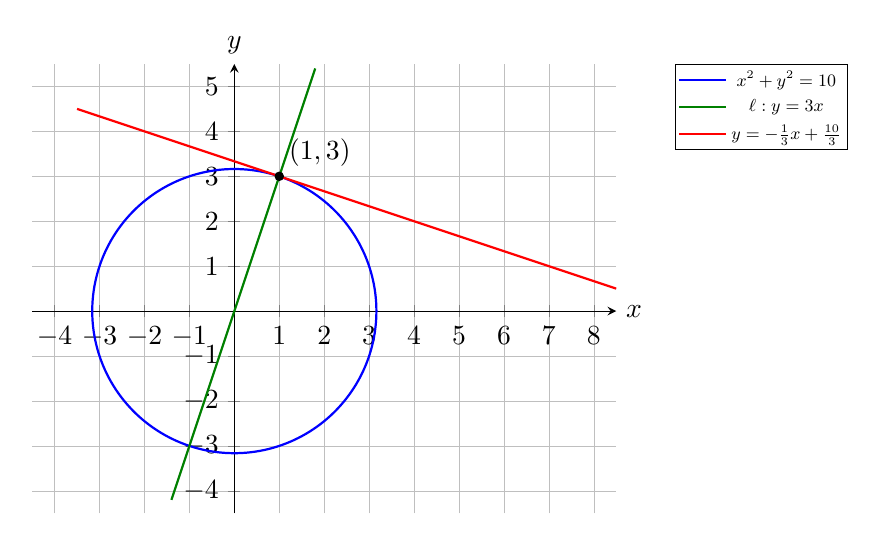
\begin{tikzpicture}
                    \begin{axis}[
        axis lines = middle,
        xlabel = $x$,
        ylabel = {$y$},
        grid=both,
        grid style={line width=.1pt, draw=gray!10},
        major grid style={line width=.2pt,draw=gray!50},
        x label style={anchor=west}, % label x ke kanan
        y label style={anchor=south}, % label y ke atas
        samples=200,
        legend style={
                at={(1.1,1)},
                anchor=north west,
                font=\small,         % mengecilkan ukuran font
                row sep=1pt,         % jarak antar baris legend
                inner sep=1pt,       % margin dalam kotak legend
                nodes={scale=0.7}    % skalakan isi legend
            },
        xtick={-4,-3,...,8},
        ytick={-4,-3,...,5},
        xmin=-4.5, xmax=8.5,
        ymin=-4.5, ymax=5.5,
        axis equal image,
        width=9cm
    ]
\addplot[domain=0:360, color=blue, thick] ({sqrt(10)*cos(x)}, {sqrt(10)*sin(x)});
\addlegendentry{$x^2+y^2=10$}
\addplot[domain=-1.4:1.8, color=green!50!black, thick, samples=2] {3*x};
\addlegendentry{$\ell: y=3x$}
\addplot[domain=-3.5:8.5, color=red, thick, samples=2] {-x/3+10/3};
\addlegendentry{$y=-\frac{1}{3}x+\frac{10}{3}$}
\draw[fill=black] (1,3) circle (1.5pt) node[above right] {$(1,3)$};
\end{axis}
                \end{tikzpicture}
            \end{center}
        \end{enumerate}
    }
    \end{jawab}

    \item \textbf{[Subbab 2.1, 2.2]} Given a function $f(x)=\sqrt{x+1}$ and $g(x)=2x-3$ on the interval $1\leq x\leq 4$.
    \begin{enumerate}
        \item Find the domain and range of $f$.
        \item Find the composite function $f(g(x))$, its domain, and its range.
    \end{enumerate}
    \begin{jawab}[domain dan range fungsi, fungsi komposisi, domain fungsi komposisi]{
        \begin{enumerate}
            \item Fungsi $f$ terdefinisi jika $x+1\geq 0$, sehingga $\colorlet{oldcolor}{.}
        \color{red}
        \setlength{\fboxrule}{1pt} \boxed{\color{oldcolor}D(f)=[-1,\infty)}\color{oldcolor}$. Karena akar kuadrat selalu tak negatif dan $\sqrt{x+1}$ membesar tanpa batas, maka $\colorlet{oldcolor}{.}
        \color{red}
        \setlength{\fboxrule}{1pt} \boxed{\color{oldcolor}R(f)=[0,\infty)}\color{oldcolor}$.
            \item Diperhatikan bahwa
            \begin{align*}
                f(g(x)) = f(2x-3) = \sqrt{(2x-3)+1} = \colorlet{oldcolor}{.}
        \color{red}
        \setlength{\fboxrule}{1pt} \boxed{\color{oldcolor}\sqrt{2x-2}}\color{oldcolor}.
            \end{align*}
            Domain dari fungsi komposisi adalah semua nilai $x$ pada domain $g$ sehingga nilai dari $g(x)$ berada pada domain $f$, yaitu
            \begin{align*}
                \colorlet{oldcolor}{.}
        \color{blue}
        \setlength{\fboxrule}{1pt} \boxed{\color{oldcolor}D(f\circ g) = \{x \in D(g) : g(x) \in D(f)\} = \{x \in [1,4] : 2x-3\geq -1\}}\color{oldcolor}.
            \end{align*}
            Syarat $2x-3\geq -1$ setara dengan $x\geq 1$, yang selalu terpenuhi untuk $x\in[1,4]$. Jadi
            \begin{align*}
                \colorlet{oldcolor}{.}
        \color{red}
        \setlength{\fboxrule}{1pt} \boxed{\color{oldcolor}D(f\circ g)=[1,4]}\color{oldcolor}.
            \end{align*}
            \textit{Catatan:} meskipun bentuk akhir $\sqrt{2x-2}$ terdefinisi untuk semua $x\geq 1$, domain komposisi tetap dibatasi oleh domain $g$, yaitu $[1,4]$.\\
            Karena $\sqrt{2x-2}$ naik pada $[1,4]$, nilai terkecilnya $0$ (di $x=1$) dan nilai terbesarnya $\sqrt{6}$ (di $x=4$). Jadi range dari $f\circ g$ adalah $\colorlet{oldcolor}{.}
        \color{red}
        \setlength{\fboxrule}{1pt} \boxed{\color{oldcolor}\left[0,\sqrt{6}\right]}\color{oldcolor}$.
        \end{enumerate}
    }
    \end{jawab}

    \item \textbf{[Subbab 3.4]} Given $f(x)=\begin{cases}
        kx^2+2, & x\leq 1\\
        4x-k, & x>1
    \end{cases}$. Find the value of $k$ such that $f$ is continuous everywhere.
    \begin{jawab}[kekontinuan, limit sepihak, fungsi sepotong-sepotong]{~\\
        Untuk $x<1$ dan $x>1$, fungsi $f$ berupa polinomial sehingga kontinu. Jadi $f$ kontinu di mana-mana jika dan hanya jika $f$ kontinu di $x=1$. Ingat kembali syarat fungsi kontinu di suatu titik \(x = a\) adalah
        \begin{enumerate}
            \item \(f(a)\) terdefinisi
            \item \(\displaystyle \lim_{x \to a} f(x)\) ada, yaitu $\displaystyle \lim_{x \to a^-} f(x) = \lim_{x \to a^+} f(x)$
            \item \(\displaystyle\lim_{x \to a} f(x) = f(a)\)
        \end{enumerate}
        Diperhatikan bahwa $\colorlet{oldcolor}{.}
        \color{blue}
        \setlength{\fboxrule}{1pt} \boxed{\color{oldcolor}f(1)=k+2~\text{terdefinisi}}\color{oldcolor}$, serta
        \begin{align*}
            \lim_{x\to 1^-}f(x)=\lim_{x\to 1^-}(kx^2+2)=k+2 \quad\text{dan}\quad \lim_{x\to 1^+}f(x)=\lim_{x\to 1^+}(4x-k)=4-k.
        \end{align*}
        Agar kontinu, haruslah $k+2=4-k$, yaitu $2k=2$, sehingga $\colorlet{oldcolor}{.}
        \color{red}
        \setlength{\fboxrule}{1pt} \boxed{\color{oldcolor}k=1}\color{oldcolor}$. Sebagai pengecekan, untuk $k=1$ diperoleh $f(1)=3$ dan kedua limit sepihak juga bernilai $3$.
    }
    \end{jawab}

    \item \textbf{[Subbab 4.3]} Write the derivative formula of $\dfrac{f}{g}$, that is $\dfrac{d}{dx}\left(\dfrac{f(x)}{g(x)}\right)$.\\
    Then, find the derivative of $\dfrac{f}{g}$ given that $f(x)=2x^2-1$ and $g(x)=x+3$ for $x\neq -3$.
    \begin{jawab}[turunan, aturan pembagian]{~\\
        Ingat kembali aturan turunan untuk pembagian fungsi, yaitu
        \[
        \colorlet{oldcolor}{.}
        \color{red}
        \setlength{\fboxrule}{1pt} \boxed{\color{oldcolor}\frac{d}{dx}\left(\frac{f(x)}{g(x)}\right) = \frac{f'(x)g(x) - f(x)g'(x)}{(g(x))^2}}\color{oldcolor}.
        \]
        Selanjutnya, kita hitung turunan dari \(f(x)\) dan \(g(x)\):
        \begin{align*}
            \colorlet{oldcolor}{.}
        \color{blue}
        \setlength{\fboxrule}{1pt} \boxed{\color{oldcolor}f'(x) = \frac{d}{dx}(2x^2-1) = 4x}\color{oldcolor}\\
            \colorlet{oldcolor}{.}
        \color{blue}
        \setlength{\fboxrule}{1pt} \boxed{\color{oldcolor}g'(x) = \frac{d}{dx}(x+3) = 1}\color{oldcolor}
        \end{align*}
        Dengan demikian, turunan dari \(\frac{f}{g}\) adalah
        \begin{align*}
            \frac{d}{dx}\left(\frac{f(x)}{g(x)}\right) &= \frac{4x(x+3)-(2x^2-1)(1)}{(x+3)^2}\\
            &= \frac{4x^2+12x-2x^2+1}{(x+3)^2}\\
            &= \colorlet{oldcolor}{.}
        \color{red}
        \setlength{\fboxrule}{1pt} \boxed{\color{oldcolor}\frac{2x^2+12x+1}{(x+3)^2}}\color{oldcolor}.
        \end{align*}
    }
    \end{jawab}

\end{enumerate}

\newpage

%%%%%%%%%%%%%%%%%%%%%%%%%%%%%%%%%%%%%%%%%%%%%%%%%%%%%%%%%%%%%%%%%%%%%%%%%%%%%%
% M2-14
\kopsoalmat{M2-14}{1-7}{Sistem Informasi, Manajemen Bisnis, Studi Pembangunan, Bdigt, Skom}{Jum'at, 07.00-09.30}{11}
\begin{enumerate}
    \item Dapatkan himpunan penyelesaian dari $\dfrac{2}{x-2}\geq\dfrac{1}{x+1}$.
    \begin{jawab}[pertidaksamaan rasional, pecahan, garis bilangan, notasi interval]{~\\
        Untuk menyelesaikan pertidaksamaan rasional, pastikan ruas kanan sudah bernilai nol (jangan dikali silang, karena tanda penyebutnya belum diketahui). Dengan mengurangkan \(\frac{1}{x+1}\) dari kedua ruas, didapatkan
        \[
        \frac{2}{x-2} - \frac{1}{x+1} \geq 0
        \]
        Selanjutnya, dengan menyamakan penyebut dan menyederhanakan bentuknya, diperoleh
        \begin{align}
            \frac{2(x+1)-(x-2)}{(x-2)(x+1)} &\geq 0\nonumber\\
            \frac{2x+2-x+2}{(x-2)(x+1)} &\geq 0\nonumber \\
            \frac{x+4}{(x-2)(x+1)} &\geq 0 \label{ineq:m2}
        \end{align}
        Didapatkan pembuat nol dari faktor-faktornya adalah
        \begin{align*}
            x+4 = 0 \quad &\vee\quad  x-2 = 0 \quad\vee\quad x+1=0\\
            \colorlet{oldcolor}{.}
        \color{blue}
        \setlength{\fboxrule}{1pt} \boxed{\color{oldcolor}x=-4}\color{oldcolor} \quad &\vee\quad \colorlet{oldcolor}{.}
        \color{blue}
        \setlength{\fboxrule}{1pt} \boxed{\color{oldcolor}x=2}\color{oldcolor} \quad\vee\quad \colorlet{oldcolor}{.}
        \color{blue}
        \setlength{\fboxrule}{1pt} \boxed{\color{oldcolor}x=-1}\color{oldcolor}
        \end{align*}
        Selanjutnya, dibuat garis bilangan dan dilakukan uji titik pada ekspresi \eqref{ineq:m2} sebagai berikut
        \begin{itemize}
            \item Untuk \(x < -4\), misalkan \(x = -5\):
            \[
            \frac{-5+4}{(-5-2)(-5+1)} = \frac{-1}{(-7)(-4)} = \frac{-1}{28} < 0
            \]
            \item Untuk \(-4 < x < -1\), misalkan \(x = -2\):
            \[
            \frac{-2+4}{(-2-2)(-2+1)} = \frac{2}{(-4)(-1)} = \frac{2}{4} > 0
            \]
            \item Untuk \(-1 < x < 2\), misalkan \(x = 0\):
            \[
            \frac{0+4}{(0-2)(0+1)} = \frac{4}{-2} < 0
            \]
            \item Untuk \(x > 2\), misalkan \(x = 3\):
            \[
            \frac{3+4}{(3-2)(3+1)} = \frac{7}{4} > 0
            \]
        \end{itemize}
        \begin{center}
           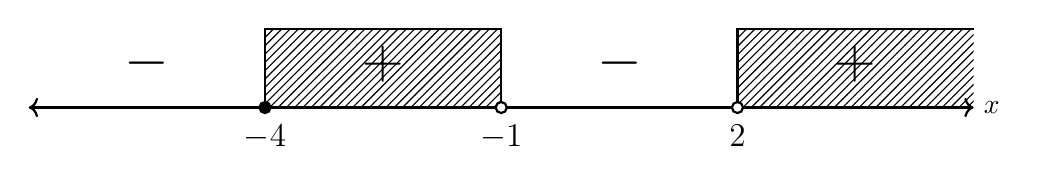
\begin{tikzpicture}
    \draw[thick,<->] (-6,0) -- (6,0) node[right] {$x$};
    \fill[pattern=north east lines] (-3,0) rectangle (0,1);
    \fill[pattern=north east lines] (3,0) rectangle (6,1);
    \draw[thick] (-3,0) -- (-3,1) -- (0,1) -- (0,0);
    \draw[thick] (3,0) -- (3,1) -- (6,1);
    \draw (-3,-0.1) node[below] {\large{$-4$}};
    \draw (0,-0.1) node[below] {\large{$-1$}};
    \draw (3,-0.1) node[below] {\large{$2$}};
    \draw (-4.5,0.2) node[above] {\huge{$-$}};
    \draw (-1.5,0.2) node[above] {\huge{$+$}};
    \draw (1.5,0.2) node[above] {\huge{$-$}};
    \draw (4.5,0.2) node[above] {\huge{$+$}};
    \draw[fill=black, thick] (-3,0) circle (2pt);
    \draw[fill=white, thick] (0,0) circle (2pt);
    \draw[fill=white, thick] (3,0) circle (2pt);
\end{tikzpicture}
        \end{center}
        Karena yang diminta adalah nilai \(x\) yang membuat pertidaksamaan \eqref{ineq:m2} lebih dari atau sama dengan nol, diambil interval yang bertanda positif beserta pembuat nol pembilang ($x=-4$). Pembuat nol penyebut ($x=-1$ dan $x=2$) tidak diikutkan karena membuat ekspresi tidak terdefinisi. Jadi himpunan penyelesaiannya adalah
        \[
        \colorlet{oldcolor}{.}
        \color{red}
        \setlength{\fboxrule}{1pt} \boxed{\color{oldcolor}\{x\in\mathbb{R} : -4\leq x<-1 \;\vee\; x>2\} = [-4,-1)\cup(2,\infty)}\color{oldcolor}.
        \]
    }
    \end{jawab}

    \item Diketahui garis $l_1$ melalui titik $(-1,2)$ dan $(3,4)$.
    \begin{enumerate}
        \item Dapatkan persamaan garis $l_2$ yang melalui titik $(2,1)$ dan tegak lurus dengan garis $l_1$.
        \item Tentukan titik potong garis $l_1$ dan $l_2$.
    \end{enumerate}
    \begin{jawab}[gradien garis, garis tegak lurus, persamaan garis, titik potong garis]{
        \begin{enumerate}
            \item Kemiringan garis yang melalui dua titik $(x_1,y_1)$ dan $(x_2,y_2)$ adalah $m = \frac{y_2 - y_1}{x_2 - x_1}$. Dengan substitusi $(-1,2)$ dan $(3,4)$, diperoleh
            \begin{align*}
                m_1 = \frac{4-2}{3-(-1)} = \frac{2}{4} = \colorlet{oldcolor}{.}
        \color{blue}
        \setlength{\fboxrule}{1pt} \boxed{\color{oldcolor}\frac{1}{2}}\color{oldcolor}.
            \end{align*}
            Dua garis saling tegak lurus jika $\colorlet{oldcolor}{.}
        \color{blue}
        \setlength{\fboxrule}{1pt} \boxed{\color{oldcolor}m_1\cdot m_2=-1}\color{oldcolor}$, sehingga $\frac{1}{2}\cdot m_2=-1$ dan diperoleh $m_2=-2$. Garis $l_2$ melalui titik $(2,1)$, sehingga dengan rumus $y - y_1 = m(x - x_1)$ diperoleh
            \begin{align*}
                y - 1 &= -2(x - 2)\\
                y &= -2x + 5.
            \end{align*}
            Jadi persamaan garis $l_2$ adalah $\colorlet{oldcolor}{.}
        \color{red}
        \setlength{\fboxrule}{1pt} \boxed{\color{oldcolor}y = -2x + 5}\color{oldcolor}$ atau $2x+y=5$.
            \item Terlebih dahulu ditentukan persamaan garis $l_1$, yaitu garis dengan gradien $\frac{1}{2}$ yang melalui titik $(-1,2)$:
            \begin{align*}
                y - 2 = \frac{1}{2}(x + 1) \implies \colorlet{oldcolor}{.}
        \color{blue}
        \setlength{\fboxrule}{1pt} \boxed{\color{oldcolor}y = \frac{1}{2}x + \frac{5}{2}}\color{oldcolor}.
            \end{align*}
            Untuk menentukan titik potong kedua garis, kita samakan persamaan kedua garis, yaitu
            \begin{align*}
                \frac{1}{2}x + \frac{5}{2} &= -2x + 5\\
                x + 5 &= -4x + 10\\
                5x &= 5 \implies x = 1.
            \end{align*}
            Substitusi $x=1$ ke persamaan $l_2$, diperoleh $y=-2(1)+5=3$ (dapat dicek pula $\frac{1}{2}(1)+\frac{5}{2}=3$). Jadi titik potong garis $l_1$ dan $l_2$ adalah $\colorlet{oldcolor}{.}
        \color{red}
        \setlength{\fboxrule}{1pt} \boxed{\color{oldcolor}(1,3)}\color{oldcolor}$.
        \end{enumerate}
    }
    \end{jawab}

    \item Diberikan SPL
    \begin{align*}
        x+2y-z &= 3\\
        2x-y+3z &= 6\\
        -x+y+2z &= 5
    \end{align*}
    \begin{enumerate}
        \item Nyatakan SPL tersebut dalam bentuk persamaan matriks $A\mathbf{x}=b$.
        \item Menggunakan eliminasi Gauss-Jordan, carilah solusi (jika ada) dari SPL tersebut.
    \end{enumerate}
    \begin{jawab}[sistem persamaan linear, matriks, eliminasi Gauss-Jordan]{
        \begin{enumerate}
            \item Koefisien dari variabel $x,y,z$ pada setiap persamaan disusun menjadi matriks $A$, variabelnya menjadi vektor $\mathbf{x}$, dan ruas kanan menjadi vektor $b$. Diperoleh
            \begin{align*}
                \colorlet{oldcolor}{.}
        \color{red}
        \setlength{\fboxrule}{1pt} \boxed{\color{oldcolor}\underbrace{\begin{bmatrix}
                    1 & 2 & -1\\
                    2 & -1 & 3\\
                    -1 & 1 & 2
                \end{bmatrix}}_{A}
                \underbrace{\begin{bmatrix}
                    x\\ y\\ z
                \end{bmatrix}}_{\mathbf{x}}
                =
                \underbrace{\begin{bmatrix}
                    3\\ 6\\ 5
                \end{bmatrix}}_{b}}\color{oldcolor}.
            \end{align*}
            \item Dibentuk matriks lengkap (\textit{augmented matrix}) $[A\,|\,b]$, kemudian dilakukan operasi baris elementer (OBE) sampai terbentuk matriks eselon baris tereduksi.
            \begin{align*}
                &\left[\begin{array}{ccc|c}
                    1 & 2 & -1 & 3\\
                    2 & -1 & 3 & 6\\
                    -1 & 1 & 2 & 5
                \end{array}\right]
                \xrightarrow[R_3 + R_1]{R_2 - 2R_1}
                \left[\begin{array}{ccc|c}
                    1 & 2 & -1 & 3\\
                    0 & -5 & 5 & 0\\
                    0 & 3 & 1 & 8
                \end{array}\right]
                \xrightarrow{-\frac{1}{5}R_2}
                \left[\begin{array}{ccc|c}
                    1 & 2 & -1 & 3\\
                    0 & 1 & -1 & 0\\
                    0 & 3 & 1 & 8
                \end{array}\right]\\
                &\xrightarrow[R_3 - 3R_2]{R_1 - 2R_2}
                \left[\begin{array}{ccc|c}
                    1 & 0 & 1 & 3\\
                    0 & 1 & -1 & 0\\
                    0 & 0 & 4 & 8
                \end{array}\right]
                \xrightarrow{\frac{1}{4}R_3}
                \left[\begin{array}{ccc|c}
                    1 & 0 & 1 & 3\\
                    0 & 1 & -1 & 0\\
                    0 & 0 & 1 & 2
                \end{array}\right]
                \xrightarrow[R_2 + R_3]{R_1 - R_3}
                \left[\begin{array}{ccc|c}
                    1 & 0 & 0 & 1\\
                    0 & 1 & 0 & 2\\
                    0 & 0 & 1 & 2
                \end{array}\right]
            \end{align*}
            Matriks terakhir sudah berbentuk eselon baris tereduksi dan setiap kolom variabel memiliki pivot, sehingga SPL memiliki solusi tunggal, yaitu $\colorlet{oldcolor}{.}
        \color{blue}
        \setlength{\fboxrule}{1pt} \boxed{\color{oldcolor}x=1}\color{oldcolor}$, $\colorlet{oldcolor}{.}
        \color{blue}
        \setlength{\fboxrule}{1pt} \boxed{\color{oldcolor}y=2}\color{oldcolor}$, dan $\colorlet{oldcolor}{.}
        \color{blue}
        \setlength{\fboxrule}{1pt} \boxed{\color{oldcolor}z=2}\color{oldcolor}$.\\
            Sebagai pengecekan, $1+2(2)-2=3$, $2(1)-2+3(2)=6$, dan $-1+2+2(2)=5$, sesuai dengan SPL. Jadi solusi dari SPL tersebut adalah $\colorlet{oldcolor}{.}
        \color{red}
        \setlength{\fboxrule}{1pt} \boxed{\color{oldcolor}(x,y,z)=(1,2,2)}\color{oldcolor}$.
        \end{enumerate}
    }
    \end{jawab}

    \item Diketahui fungsi $f(x)=x^2-4x-5$.
    \begin{enumerate}
        \item Dapatkan domain dan range dari $f(x)$.
        \item Sketsa grafik $f(x)$ beserta titik puncak dan titik potongnya dengan sumbu koordinat.
    \end{enumerate}
    \begin{jawab}[fungsi kuadrat, melengkapkan kuadrat, domain dan range, sketsa grafik]{
        \begin{enumerate}
            \item Karena $f$ adalah fungsi polinomial (fungsi kuadrat), maka $f$ terdefinisi untuk setiap bilangan real, sehingga $\colorlet{oldcolor}{.}
        \color{red}
        \setlength{\fboxrule}{1pt} \boxed{\color{oldcolor}D(f)=\mathbb{R}}\color{oldcolor}$. Selanjutnya, dengan melengkapkan kuadrat, diperoleh
            \begin{align*}
                f(x) = x^2-4x-5 = (x^2-4x+4)-4-5 = \colorlet{oldcolor}{.}
        \color{blue}
        \setlength{\fboxrule}{1pt} \boxed{\color{oldcolor}(x-2)^2-9}\color{oldcolor}.
            \end{align*}
            Karena $(x-2)^2\geq 0$ untuk setiap $x$, maka $f(x)\geq -9$, dengan nilai minimum $-9$ dicapai saat $x=2$. Grafiknya terbuka ke atas sehingga nilainya membesar tanpa batas. Jadi
            \begin{align*}
                \colorlet{oldcolor}{.}
        \color{red}
        \setlength{\fboxrule}{1pt} \boxed{\color{oldcolor}R(f)=\{y\in\mathbb{R} : y\geq -9\}=[-9,\infty)}\color{oldcolor}.
            \end{align*}
            \item Dari (a), titik puncak parabola adalah $\colorlet{oldcolor}{.}
        \color{blue}
        \setlength{\fboxrule}{1pt} \boxed{\color{oldcolor}(2,-9)}\color{oldcolor}$, dan karena koefisien $x^2$ positif, parabola terbuka ke atas.
            \begin{itemize}
                \item Titik potong dengan sumbu-$x$ ($y=0$): $x^2-4x-5=(x-5)(x+1)=0$, sehingga $x=5$ atau $x=-1$, yaitu titik $\colorlet{oldcolor}{.}
        \color{blue}
        \setlength{\fboxrule}{1pt} \boxed{\color{oldcolor}(-1,0)}\color{oldcolor}$ dan $\colorlet{oldcolor}{.}
        \color{blue}
        \setlength{\fboxrule}{1pt} \boxed{\color{oldcolor}(5,0)}\color{oldcolor}$.
                \item Titik potong dengan sumbu-$y$ ($x=0$): $f(0)=-5$, yaitu titik $\colorlet{oldcolor}{.}
        \color{blue}
        \setlength{\fboxrule}{1pt} \boxed{\color{oldcolor}(0,-5)}\color{oldcolor}$.
            \end{itemize}
            Sketsa grafiknya adalah sebagai berikut:
            \begin{center}
                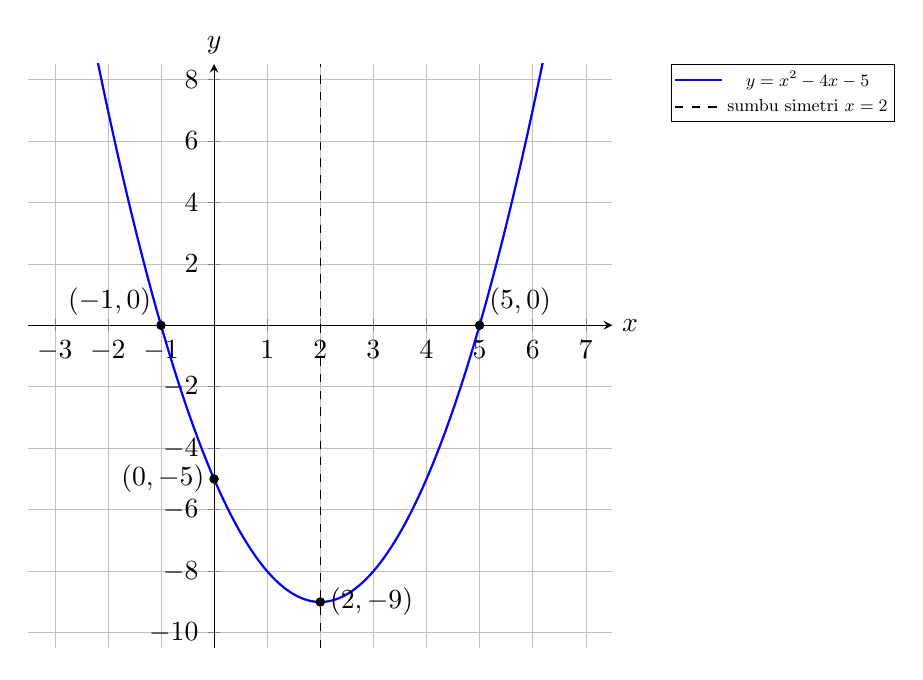
\begin{tikzpicture}
                    \begin{axis}[
        axis lines = middle,
        xlabel = $x$,
        ylabel = {$y$},
        grid=both,
        grid style={line width=.1pt, draw=gray!10},
        major grid style={line width=.2pt,draw=gray!50},
        x label style={anchor=west}, % label x ke kanan
        y label style={anchor=south}, % label y ke atas
        samples=200,
        legend style={
                at={(1.1,1)},
                anchor=north west,
                font=\small,         % mengecilkan ukuran font
                row sep=1pt,         % jarak antar baris legend
                inner sep=1pt,       % margin dalam kotak legend
                nodes={scale=0.7}    % skalakan isi legend
            },
        xtick={-3,-2,...,7},
        ytick={-10,-8,...,8},
        xmin=-3.5, xmax=7.5,
        ymin=-10.5, ymax=8.5,
        width=9cm,
        height=9cm
    ]
\addplot[domain=-2.4:6.4, color=blue, thick] {x^2-4*x-5};
\addlegendentry{$y=x^2-4x-5$}
\addplot[color=black, dashed] coordinates {(2,-10.5) (2,8.5)};
\addlegendentry{sumbu simetri $x=2$}
\draw[fill=black] (2,-9) circle (1.5pt) node[right] {$(2,-9)$};
\draw[fill=black] (-1,0) circle (1.5pt) node[above left] {$(-1,0)$};
\draw[fill=black] (5,0) circle (1.5pt) node[above right] {$(5,0)$};
\draw[fill=black] (0,-5) circle (1.5pt) node[left] {$(0,-5)$};
\end{axis}
                \end{tikzpicture}
            \end{center}
        \end{enumerate}
    }
    \end{jawab}

    \item Diberikan sistem persamaan fungsi permintaan dan penawaran (\textit{supply and demand})
    \begin{align*}
        3P &= -Q_d+150\\
        2P &= Q_s+25
    \end{align*}
    dengan $P,Q_d,Q_s$ masing-masing adalah harga, jumlah permintaan (\textit{demand}), dan jumlah penawaran (\textit{supply}).
    \begin{enumerate}
        \item Tentukan harga dan jumlah barang di titik equilibrium.
        \item Misalkan pemerintah memberikan pajak sebesar 5 untuk masing-masing barang. Tentukan persamaan fungsi penawaran setelah dikenakan pajak, titik equilibrium yang baru, dan pembagian pembayaran pajaknya.
        \item Gambarkan/sket kurva permintaan dan penawaran (sebelum dan sesudah pajak) beserta titik keseimbangannya.
    \end{enumerate}
    \begin{jawab}[fungsi permintaan, fungsi penawaran, titik keseimbangan pasar, pajak per unit]{~\\
        Dari sistem persamaan yang diberikan, fungsi permintaan dan penawaran dapat ditulis sebagai
        \begin{align*}
            \colorlet{oldcolor}{.}
        \color{blue}
        \setlength{\fboxrule}{1pt} \boxed{\color{oldcolor}Q_d = 150 - 3P}\color{oldcolor} \quad\text{dan}\quad \colorlet{oldcolor}{.}
        \color{blue}
        \setlength{\fboxrule}{1pt} \boxed{\color{oldcolor}Q_s = 2P - 25}\color{oldcolor}.
        \end{align*}
        \begin{enumerate}
            \item Titik keseimbangan (\textit{equilibrium}) terjadi saat jumlah permintaan sama dengan jumlah penawaran, yaitu $\colorlet{oldcolor}{.}
        \color{blue}
        \setlength{\fboxrule}{1pt} \boxed{\color{oldcolor}Q_d=Q_s}\color{oldcolor}$. Diperoleh
            \begin{align*}
                150 - 3P &= 2P - 25\\
                175 &= 5P\\
                P &= 35.
            \end{align*}
            Substitusi $P=35$ ke fungsi permintaan, diperoleh $Q = 150 - 3(35) = 150 - 105 = 45$ (dapat dicek pula $Q_s=2(35)-25=45$). Jadi titik keseimbangannya adalah $\colorlet{oldcolor}{.}
        \color{red}
        \setlength{\fboxrule}{1pt} \boxed{\color{oldcolor}E(Q,P)=(45,35)}\color{oldcolor}$, yaitu harga keseimbangan $35$ dengan jumlah barang $45$ unit.
            \item Pajak per unit $t=5$ dibebankan kepada produsen, sehingga untuk menawarkan jumlah barang yang sama, produsen menaikkan harga sebesar $5$. Dari fungsi penawaran semula $P=\frac{Q+25}{2}$, fungsi penawaran setelah pajak adalah
            \begin{align*}
                P = \frac{Q+25}{2} + 5 \iff 2P = Q + 35 \iff \colorlet{oldcolor}{.}
        \color{red}
        \setlength{\fboxrule}{1pt} \boxed{\color{oldcolor}Q_s' = 2P - 35}\color{oldcolor}.
            \end{align*}
            Titik keseimbangan baru diperoleh dari $Q_d=Q_s'$, yaitu
            \begin{align*}
                150 - 3P &= 2P - 35\\
                185 &= 5P\\
                P &= 37,
            \end{align*}
            dan $Q = 150 - 3(37) = 150 - 111 = 39$. Jadi titik keseimbangan setelah pajak adalah
            \begin{align*}
                \colorlet{oldcolor}{.}
        \color{red}
        \setlength{\fboxrule}{1pt} \boxed{\color{oldcolor}E'(Q,P)=(39,37)}\color{oldcolor}.
            \end{align*}
            Selanjutnya, pembagian pembayaran pajak per unit adalah sebagai berikut.
            \begin{itemize}
                \item Pajak yang ditanggung konsumen per unit adalah kenaikan harga yang dibayar konsumen, yaitu $37-35=2$.
                \item Pajak yang ditanggung produsen per unit adalah sisanya, yaitu $5-2=3$.
            \end{itemize}
            Dengan jumlah barang setelah pajak sebanyak $39$ unit, total pajak yang diterima pemerintah adalah $5\times 39=195$, dengan pembagian
            \[
            \colorlet{oldcolor}{.}
        \color{red}
        \setlength{\fboxrule}{1pt} \boxed{\color{oldcolor}\text{konsumen: } 2\times 39 = 78, \quad \text{produsen: } 3\times 39 = 117}\color{oldcolor}.
            \]
            \item Dalam ekonomi, sumbu mendatar menyatakan jumlah barang $Q$ dan sumbu tegak menyatakan harga $P$. Sebagai bantuan menggambar:
            \begin{itemize}
                \item Kurva permintaan $P=\frac{150-Q}{3}$ melalui titik $(0,50)$ dan $(150,0)$, dan turun dari kiri ke kanan.
                \item Kurva penawaran sebelum pajak $P=\frac{Q+25}{2}$ melalui titik $(0;12{,}5)$ dan $(45,35)$, dan naik dari kiri ke kanan.
                \item Kurva penawaran setelah pajak $P=\frac{Q+35}{2}$ melalui titik $(0;17{,}5)$ dan $(39,37)$, yaitu kurva penawaran semula yang bergeser $5$ satuan ke atas.
            \end{itemize}
            Sketsa kurva permintaan, penawaran, dan titik keseimbangannya adalah sebagai berikut
            \begin{center}
                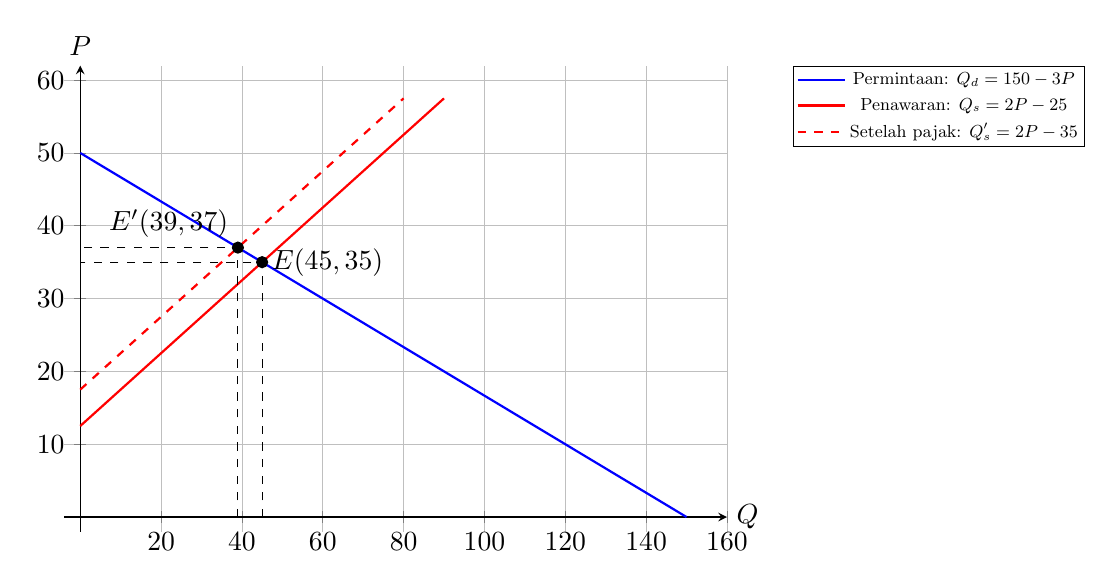
\begin{tikzpicture}
                    \begin{axis}[
        axis lines = middle,
        xlabel = $x$,
        ylabel = {$y$},
        grid=both,
        grid style={line width=.1pt, draw=gray!10},
        major grid style={line width=.2pt,draw=gray!50},
        x label style={anchor=west}, % label x ke kanan
        y label style={anchor=south}, % label y ke atas
        samples=200,
        legend style={
                at={(1.1,1)},
                anchor=north west,
                font=\small,         % mengecilkan ukuran font
                row sep=1pt,         % jarak antar baris legend
                inner sep=1pt,       % margin dalam kotak legend
                nodes={scale=0.7}    % skalakan isi legend
            },
        xlabel = $Q$,
        ylabel = {$P$},
        xtick={0,20,...,160},
        ytick={0,10,...,60},
        xmin=-4, xmax=160,
        ymin=-2, ymax=62,
        width=10cm,
        height=7.5cm
    ]
\addplot[domain=0:150, color=blue, thick, samples=2] {(150-x)/3};
\addlegendentry{Permintaan: $Q_d=150-3P$}
\addplot[domain=0:90, color=red, thick, samples=2] {(x+25)/2};
\addlegendentry{Penawaran: $Q_s=2P-25$}
\addplot[domain=0:80, color=red, thick, dashed, samples=2] {(x+35)/2};
\addlegendentry{Setelah pajak: $Q_s'=2P-35$}
\draw[fill=black] (45,35) circle (2pt) node[right] {$E(45,35)$};
\draw[fill=black] (39,37) circle (2pt) node[above left] {$E'(39,37)$};
\draw[dashed] (45,0) -- (45,35) -- (0,35);
\draw[dashed] (39,0) -- (39,37) -- (0,37);
\end{axis}
                \end{tikzpicture}
            \end{center}
        \end{enumerate}
    }
    \end{jawab}
\end{enumerate}

\newpage

%%%%%%%%%%%%%%%%%%%%%%%%%%%%%%%%%%%%%%%%%%%%%%%%%%%%%%%%%%%%%%%%%%%%%%%%%%%%%%
% M2-iup
\kopsoalmatiup{M2-iup}{8, 9}{Information Systems, Business Management}{Friday, 07.00-09.30}{11}
\begin{enumerate}
    \item Find the solution set of $\dfrac{3}{x+2}\leq\dfrac{1}{x-2}$.
    \begin{jawab}[pertidaksamaan rasional, pecahan, garis bilangan, notasi interval]{~\\
        Untuk menyelesaikan pertidaksamaan rasional, pastikan ruas kanan sudah bernilai nol (jangan dikali silang, karena tanda penyebutnya belum diketahui). Dengan mengurangkan \(\frac{1}{x-2}\) dari kedua ruas, didapatkan
        \[
        \frac{3}{x+2} - \frac{1}{x-2} \leq 0
        \]
        Selanjutnya, dengan menyamakan penyebut dan menyederhanakan bentuknya, diperoleh
        \begin{align}
            \frac{3(x-2)-(x+2)}{(x+2)(x-2)} &\leq 0\nonumber\\
            \frac{3x-6-x-2}{(x+2)(x-2)} &\leq 0\nonumber \\
            \frac{2(x-4)}{(x+2)(x-2)} &\leq 0 \label{ineq:m2iup}
        \end{align}
        Didapatkan pembuat nol dari faktor-faktornya adalah
        \begin{align*}
            x-4 = 0 \quad &\vee\quad  x+2 = 0 \quad\vee\quad x-2=0\\
            \colorlet{oldcolor}{.}
        \color{blue}
        \setlength{\fboxrule}{1pt} \boxed{\color{oldcolor}x=4}\color{oldcolor} \quad &\vee\quad \colorlet{oldcolor}{.}
        \color{blue}
        \setlength{\fboxrule}{1pt} \boxed{\color{oldcolor}x=-2}\color{oldcolor} \quad\vee\quad \colorlet{oldcolor}{.}
        \color{blue}
        \setlength{\fboxrule}{1pt} \boxed{\color{oldcolor}x=2}\color{oldcolor}
        \end{align*}
        Selanjutnya, dibuat garis bilangan dan dilakukan uji titik pada ekspresi \eqref{ineq:m2iup} sebagai berikut
        \begin{itemize}
            \item Untuk \(x < -2\), misalkan \(x = -3\):
            \[
            \frac{2(-3-4)}{(-3+2)(-3-2)} = \frac{-14}{(-1)(-5)} = \frac{-14}{5} < 0
            \]
            \item Untuk \(-2 < x < 2\), misalkan \(x = 0\):
            \[
            \frac{2(0-4)}{(0+2)(0-2)} = \frac{-8}{-4} > 0
            \]
            \item Untuk \(2 < x < 4\), misalkan \(x = 3\):
            \[
            \frac{2(3-4)}{(3+2)(3-2)} = \frac{-2}{5} < 0
            \]
            \item Untuk \(x > 4\), misalkan \(x = 5\):
            \[
            \frac{2(5-4)}{(5+2)(5-2)} = \frac{2}{21} > 0
            \]
        \end{itemize}
        \begin{center}
           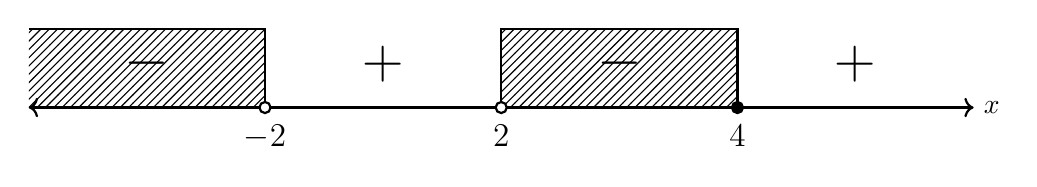
\begin{tikzpicture}
    \draw[thick,<->] (-6,0) -- (6,0) node[right] {$x$};
    \fill[pattern=north east lines] (-6,0) rectangle (-3,1);
    \fill[pattern=north east lines] (0,0) rectangle (3,1);
    \draw[thick] (-6,1) -- (-3,1) -- (-3,0);
    \draw[thick] (0,0) -- (0,1) -- (3,1) -- (3,0);
    \draw (-3,-0.1) node[below] {\large{$-2$}};
    \draw (0,-0.1) node[below] {\large{$2$}};
    \draw (3,-0.1) node[below] {\large{$4$}};
    \draw (-4.5,0.2) node[above] {\huge{$-$}};
    \draw (-1.5,0.2) node[above] {\huge{$+$}};
    \draw (1.5,0.2) node[above] {\huge{$-$}};
    \draw (4.5,0.2) node[above] {\huge{$+$}};
    \draw[fill=white, thick] (-3,0) circle (2pt);
    \draw[fill=white, thick] (0,0) circle (2pt);
    \draw[fill=black, thick] (3,0) circle (2pt);
\end{tikzpicture}
        \end{center}
        Karena yang diminta adalah nilai \(x\) yang membuat pertidaksamaan \eqref{ineq:m2iup} kurang dari atau sama dengan nol, diambil interval yang bertanda negatif beserta pembuat nol pembilang ($x=4$). Pembuat nol penyebut ($x=-2$ dan $x=2$) tidak diikutkan karena membuat ekspresi tidak terdefinisi. Jadi himpunan penyelesaiannya adalah
        \[
        \colorlet{oldcolor}{.}
        \color{red}
        \setlength{\fboxrule}{1pt} \boxed{\color{oldcolor}\{x\in\mathbb{R} : x<-2 \;\vee\; 2<x\leq 4\} = (-\infty,-2)\cup(2,4]}\color{oldcolor}.
        \]
    }
    \end{jawab}

    \item \begin{enumerate}
        \item Determine the value of $k$ such that the line $\ell_1: kx+2y=7$ is perpendicular to the line $\ell_2: 4x-6y=1$.
        \item Using the value of $k$ in (a), find the equation of the line passing through $(1,2)$ that is parallel to $\ell_1$.
    \end{enumerate}
    \begin{jawab}[gradien garis, garis tegak lurus, garis sejajar, persamaan garis]{
        \begin{enumerate}
            \item Ingat kembali bahwa garis $ax+by=c$ dapat ditulis menjadi $y=-\frac{a}{b}x+\frac{c}{b}$, sehingga gradiennya adalah $m=-\frac{a}{b}$. Diperoleh
            \begin{align*}
                \ell_1: kx+2y=7 \implies y = -\frac{k}{2}x + \frac{7}{2} \implies \colorlet{oldcolor}{.}
        \color{blue}
        \setlength{\fboxrule}{1pt} \boxed{\color{oldcolor}m_1 = -\frac{k}{2}}\color{oldcolor},\\
                \ell_2: 4x-6y=1 \implies y = \frac{2}{3}x - \frac{1}{6} \implies \colorlet{oldcolor}{.}
        \color{blue}
        \setlength{\fboxrule}{1pt} \boxed{\color{oldcolor}m_2 = \frac{2}{3}}\color{oldcolor}.
            \end{align*}
            Dua garis saling tegak lurus jika $m_1\cdot m_2=-1$, sehingga
            \begin{align*}
                -\frac{k}{2}\cdot\frac{2}{3} = -1 \implies -\frac{k}{3} = -1 \implies k=\colorlet{oldcolor}{.}
        \color{red}
        \setlength{\fboxrule}{1pt} \boxed{\color{oldcolor}3}\color{oldcolor}.
            \end{align*}
            \item Untuk $k=3$, garis $\ell_1$ adalah $3x+2y=7$ dengan gradien $m_1=-\frac{3}{2}$. Dua garis sejajar memiliki gradien yang sama, sehingga garis yang dicari memiliki gradien $-\frac{3}{2}$ dan melalui titik $(1,2)$. Dengan rumus $y - y_1 = m(x - x_1)$ diperoleh
            \begin{align*}
                y - 2 &= -\frac{3}{2}(x - 1)\\
                y &= -\frac{3}{2}x + \frac{3}{2} + 2\\
                y &= -\frac{3}{2}x + \frac{7}{2}.
            \end{align*}
            Jadi persamaan garisnya adalah $\colorlet{oldcolor}{.}
        \color{red}
        \setlength{\fboxrule}{1pt} \boxed{\color{oldcolor}y = -\frac{3}{2}x + \frac{7}{2}}\color{oldcolor}$ atau $3x+2y=7$.\\
            \textit{Catatan:} garis yang diperoleh ternyata sama dengan $\ell_1$ itu sendiri, karena titik $(1,2)$ terletak pada $\ell_1$, yaitu $3(1)+2(2)=7$. Satu-satunya garis yang sejajar $\ell_1$ dan melalui titik pada $\ell_1$ adalah $\ell_1$ sendiri (garis yang berimpit).
        \end{enumerate}
    }
    \end{jawab}

    \item Given the system of linear equations
    \begin{align*}
        2x+y-z &= 3\\
        x-y+2z &= 1\\
        3x+2y+z &= 8
    \end{align*}
    \begin{enumerate}
        \item Write the system in the matrix equation form $A\mathbf{x}=b$.
        \item Using Gauss-Jordan elimination, find the solution (if any) of the system.
    \end{enumerate}
    \begin{jawab}[sistem persamaan linear, matriks, eliminasi Gauss-Jordan]{
        \begin{enumerate}
            \item Koefisien dari variabel $x,y,z$ pada setiap persamaan disusun menjadi matriks $A$, variabelnya menjadi vektor $\mathbf{x}$, dan ruas kanan menjadi vektor $b$. Diperoleh
            \begin{align*}
                \colorlet{oldcolor}{.}
        \color{red}
        \setlength{\fboxrule}{1pt} \boxed{\color{oldcolor}\underbrace{\begin{bmatrix}
                    2 & 1 & -1\\
                    1 & -1 & 2\\
                    3 & 2 & 1
                \end{bmatrix}}_{A}
                \underbrace{\begin{bmatrix}
                    x\\ y\\ z
                \end{bmatrix}}_{\mathbf{x}}
                =
                \underbrace{\begin{bmatrix}
                    3\\ 1\\ 8
                \end{bmatrix}}_{b}}\color{oldcolor}.
            \end{align*}
            \item Dibentuk matriks lengkap (\textit{augmented matrix}) $[A\,|\,b]$, kemudian dilakukan operasi baris elementer (OBE) sampai terbentuk matriks eselon baris tereduksi. Agar pivot pertama bernilai $1$, baris pertama dan kedua ditukar terlebih dahulu.
            \begin{align*}
                &\left[\begin{array}{ccc|c}
                    2 & 1 & -1 & 3\\
                    1 & -1 & 2 & 1\\
                    3 & 2 & 1 & 8
                \end{array}\right]
                \xrightarrow{R_1 \leftrightarrow R_2}
                \left[\begin{array}{ccc|c}
                    1 & -1 & 2 & 1\\
                    2 & 1 & -1 & 3\\
                    3 & 2 & 1 & 8
                \end{array}\right]
                \xrightarrow[R_3 - 3R_1]{R_2 - 2R_1}
                \left[\begin{array}{ccc|c}
                    1 & -1 & 2 & 1\\
                    0 & 3 & -5 & 1\\
                    0 & 5 & -5 & 5
                \end{array}\right]\\
                &\xrightarrow[R_2 \leftrightarrow R_3]{\frac{1}{5}R_3}
                \left[\begin{array}{ccc|c}
                    1 & -1 & 2 & 1\\
                    0 & 1 & -1 & 1\\
                    0 & 3 & -5 & 1
                \end{array}\right]
                \xrightarrow[R_3 - 3R_2]{R_1 + R_2}
                \left[\begin{array}{ccc|c}
                    1 & 0 & 1 & 2\\
                    0 & 1 & -1 & 1\\
                    0 & 0 & -2 & -2
                \end{array}\right]
                \xrightarrow{-\frac{1}{2}R_3}
                \left[\begin{array}{ccc|c}
                    1 & 0 & 1 & 2\\
                    0 & 1 & -1 & 1\\
                    0 & 0 & 1 & 1
                \end{array}\right]\\
                &\xrightarrow[R_2 + R_3]{R_1 - R_3}
                \left[\begin{array}{ccc|c}
                    1 & 0 & 0 & 1\\
                    0 & 1 & 0 & 2\\
                    0 & 0 & 1 & 1
                \end{array}\right]
            \end{align*}
            Matriks terakhir sudah berbentuk eselon baris tereduksi dan setiap kolom variabel memiliki pivot, sehingga SPL memiliki solusi tunggal, yaitu $\colorlet{oldcolor}{.}
        \color{blue}
        \setlength{\fboxrule}{1pt} \boxed{\color{oldcolor}x=1}\color{oldcolor}$, $\colorlet{oldcolor}{.}
        \color{blue}
        \setlength{\fboxrule}{1pt} \boxed{\color{oldcolor}y=2}\color{oldcolor}$, dan $\colorlet{oldcolor}{.}
        \color{blue}
        \setlength{\fboxrule}{1pt} \boxed{\color{oldcolor}z=1}\color{oldcolor}$.\\
            Sebagai pengecekan, $2(1)+2-1=3$, $1-2+2(1)=1$, dan $3(1)+2(2)+1=8$, sesuai dengan SPL. Jadi solusi dari SPL tersebut adalah $\colorlet{oldcolor}{.}
        \color{red}
        \setlength{\fboxrule}{1pt} \boxed{\color{oldcolor}(x,y,z)=(1,2,1)}\color{oldcolor}$.
        \end{enumerate}
    }
    \end{jawab}

    \item Given the function $f(x)=-x^2+4x+5$.
    \begin{enumerate}
        \item Find the domain and range of $f(x)$.
        \item Sketch the graph of $f(x)$ including its vertex and its intersection points with the coordinate axes.
    \end{enumerate}
    \begin{jawab}[fungsi kuadrat, melengkapkan kuadrat, domain dan range, sketsa grafik]{
        \begin{enumerate}
            \item Karena $f$ adalah fungsi polinomial (fungsi kuadrat), maka $f$ terdefinisi untuk setiap bilangan real, sehingga $\colorlet{oldcolor}{.}
        \color{red}
        \setlength{\fboxrule}{1pt} \boxed{\color{oldcolor}D(f)=\mathbb{R}}\color{oldcolor}$. Selanjutnya, dengan melengkapkan kuadrat, diperoleh
            \begin{align*}
                f(x) = -x^2+4x+5 = -(x^2-4x+4)+4+5 = \colorlet{oldcolor}{.}
        \color{blue}
        \setlength{\fboxrule}{1pt} \boxed{\color{oldcolor}-(x-2)^2+9}\color{oldcolor}.
            \end{align*}
            Karena $-(x-2)^2\leq 0$ untuk setiap $x$, maka $f(x)\leq 9$, dengan nilai maksimum $9$ dicapai saat $x=2$. Grafiknya terbuka ke bawah sehingga nilainya mengecil tanpa batas. Jadi
            \begin{align*}
                \colorlet{oldcolor}{.}
        \color{red}
        \setlength{\fboxrule}{1pt} \boxed{\color{oldcolor}R(f)=\{y\in\mathbb{R} : y\leq 9\}=(-\infty,9]}\color{oldcolor}.
            \end{align*}
            \item Dari (a), titik puncak parabola adalah $\colorlet{oldcolor}{.}
        \color{blue}
        \setlength{\fboxrule}{1pt} \boxed{\color{oldcolor}(2,9)}\color{oldcolor}$, dan karena koefisien $x^2$ negatif, parabola terbuka ke bawah.
            \begin{itemize}
                \item Titik potong dengan sumbu-$x$ ($y=0$): $-x^2+4x+5=-(x-5)(x+1)=0$, sehingga $x=5$ atau $x=-1$, yaitu titik $\colorlet{oldcolor}{.}
        \color{blue}
        \setlength{\fboxrule}{1pt} \boxed{\color{oldcolor}(-1,0)}\color{oldcolor}$ dan $\colorlet{oldcolor}{.}
        \color{blue}
        \setlength{\fboxrule}{1pt} \boxed{\color{oldcolor}(5,0)}\color{oldcolor}$.
                \item Titik potong dengan sumbu-$y$ ($x=0$): $f(0)=5$, yaitu titik $\colorlet{oldcolor}{.}
        \color{blue}
        \setlength{\fboxrule}{1pt} \boxed{\color{oldcolor}(0,5)}\color{oldcolor}$.
            \end{itemize}
            Sketsa grafiknya adalah sebagai berikut:
            \begin{center}
                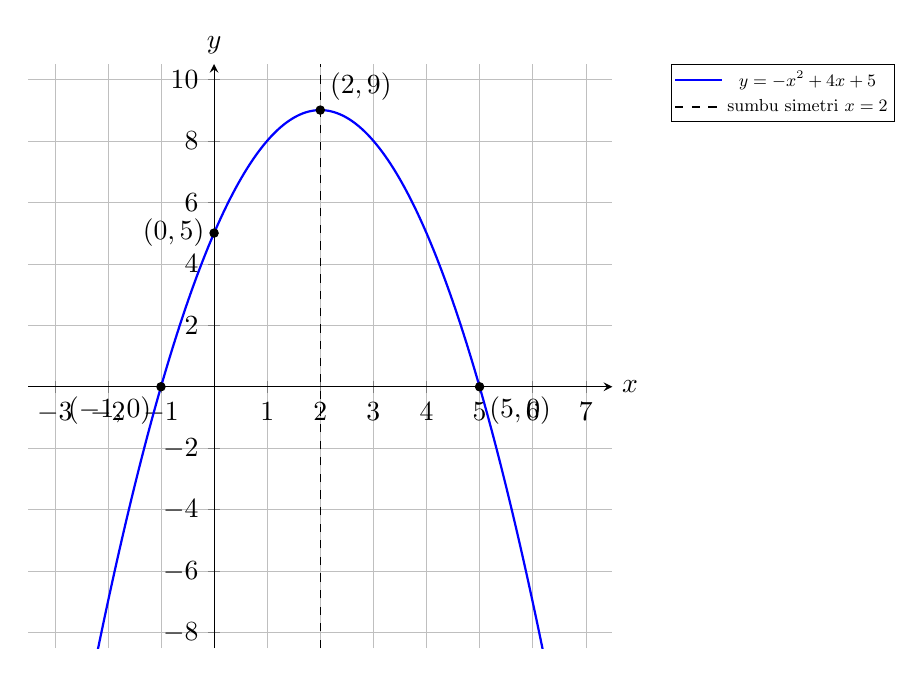
\begin{tikzpicture}
                    \begin{axis}[
        axis lines = middle,
        xlabel = $x$,
        ylabel = {$y$},
        grid=both,
        grid style={line width=.1pt, draw=gray!10},
        major grid style={line width=.2pt,draw=gray!50},
        x label style={anchor=west}, % label x ke kanan
        y label style={anchor=south}, % label y ke atas
        samples=200,
        legend style={
                at={(1.1,1)},
                anchor=north west,
                font=\small,         % mengecilkan ukuran font
                row sep=1pt,         % jarak antar baris legend
                inner sep=1pt,       % margin dalam kotak legend
                nodes={scale=0.7}    % skalakan isi legend
            },
        xtick={-3,-2,...,7},
        ytick={-8,-6,...,10},
        xmin=-3.5, xmax=7.5,
        ymin=-8.5, ymax=10.5,
        width=9cm,
        height=9cm
    ]
\addplot[domain=-2.3:6.3, color=blue, thick] {-x^2+4*x+5};
\addlegendentry{$y=-x^2+4x+5$}
\addplot[color=black, dashed] coordinates {(2,-8.5) (2,10.5)};
\addlegendentry{sumbu simetri $x=2$}
\draw[fill=black] (2,9) circle (1.5pt) node[above right] {$(2,9)$};
\draw[fill=black] (-1,0) circle (1.5pt) node[below left] {$(-1,0)$};
\draw[fill=black] (5,0) circle (1.5pt) node[below right] {$(5,0)$};
\draw[fill=black] (0,5) circle (1.5pt) node[left] {$(0,5)$};
\end{axis}
                \end{tikzpicture}
            \end{center}
        \end{enumerate}
    }
    \end{jawab}

    \item Given the demand and supply functions
    \begin{align*}
        4P &= -Q_d+140\\
        3P &= Q_s+14
    \end{align*}
    where $P,Q_d,Q_s$ are the price, the quantity demanded, and the quantity supplied, respectively.
    \begin{enumerate}
        \item Find the equilibrium price and quantity.
        \item Suppose the government imposes a tax of 7 per unit. Find the supply function after tax, the new equilibrium point, and how the tax burden is shared between consumers and producers.
        \item Sketch the demand and supply curves (before and after tax) and the equilibrium points.
    \end{enumerate}
    \begin{jawab}[fungsi permintaan, fungsi penawaran, titik keseimbangan pasar, pajak per unit]{~\\
        Dari sistem persamaan yang diberikan, fungsi permintaan dan penawaran dapat ditulis sebagai
        \begin{align*}
            \colorlet{oldcolor}{.}
        \color{blue}
        \setlength{\fboxrule}{1pt} \boxed{\color{oldcolor}Q_d = 140 - 4P}\color{oldcolor} \quad\text{dan}\quad \colorlet{oldcolor}{.}
        \color{blue}
        \setlength{\fboxrule}{1pt} \boxed{\color{oldcolor}Q_s = 3P - 14}\color{oldcolor}.
        \end{align*}
        \begin{enumerate}
            \item Titik keseimbangan (\textit{equilibrium}) terjadi saat jumlah permintaan sama dengan jumlah penawaran, yaitu $\colorlet{oldcolor}{.}
        \color{blue}
        \setlength{\fboxrule}{1pt} \boxed{\color{oldcolor}Q_d=Q_s}\color{oldcolor}$. Diperoleh
            \begin{align*}
                140 - 4P &= 3P - 14\\
                154 &= 7P\\
                P &= 22.
            \end{align*}
            Substitusi $P=22$ ke fungsi permintaan, diperoleh $Q = 140 - 4(22) = 140 - 88 = 52$ (dapat dicek pula $Q_s=3(22)-14=52$). Jadi titik keseimbangannya adalah $\colorlet{oldcolor}{.}
        \color{red}
        \setlength{\fboxrule}{1pt} \boxed{\color{oldcolor}E(Q,P)=(52,22)}\color{oldcolor}$, yaitu harga keseimbangan $22$ dengan jumlah barang $52$ unit.
            \item Pajak per unit $t=7$ dibebankan kepada produsen, sehingga untuk menawarkan jumlah barang yang sama, produsen menaikkan harga sebesar $7$. Dari fungsi penawaran semula $P=\frac{Q+14}{3}$, fungsi penawaran setelah pajak adalah
            \begin{align*}
                P = \frac{Q+14}{3} + 7 \iff 3P = Q + 35 \iff \colorlet{oldcolor}{.}
        \color{red}
        \setlength{\fboxrule}{1pt} \boxed{\color{oldcolor}Q_s' = 3P - 35}\color{oldcolor}.
            \end{align*}
            Titik keseimbangan baru diperoleh dari $Q_d=Q_s'$, yaitu
            \begin{align*}
                140 - 4P &= 3P - 35\\
                175 &= 7P\\
                P &= 25,
            \end{align*}
            dan $Q = 140 - 4(25) = 140 - 100 = 40$. Jadi titik keseimbangan setelah pajak adalah
            \begin{align*}
                \colorlet{oldcolor}{.}
        \color{red}
        \setlength{\fboxrule}{1pt} \boxed{\color{oldcolor}E'(Q,P)=(40,25)}\color{oldcolor}.
            \end{align*}
            Selanjutnya, pembagian pembayaran pajak per unit adalah sebagai berikut.
            \begin{itemize}
                \item Pajak yang ditanggung konsumen per unit adalah kenaikan harga yang dibayar konsumen, yaitu $25-22=3$.
                \item Pajak yang ditanggung produsen per unit adalah sisanya, yaitu $7-3=4$.
            \end{itemize}
            Dengan jumlah barang setelah pajak sebanyak $40$ unit, total pajak yang diterima pemerintah adalah $7\times 40=280$, dengan pembagian
            \[
            \colorlet{oldcolor}{.}
        \color{red}
        \setlength{\fboxrule}{1pt} \boxed{\color{oldcolor}\text{konsumen: } 3\times 40 = 120, \quad \text{produsen: } 4\times 40 = 160}\color{oldcolor}.
            \]
            \item Dalam ekonomi, sumbu mendatar menyatakan jumlah barang $Q$ dan sumbu tegak menyatakan harga $P$. Sebagai bantuan menggambar:
            \begin{itemize}
                \item Kurva permintaan $P=\frac{140-Q}{4}$ melalui titik $(0,35)$ dan $(140,0)$, dan turun dari kiri ke kanan.
                \item Kurva penawaran sebelum pajak $P=\frac{Q+14}{3}$ melalui titik $\left(0,\frac{14}{3}\right)$ dan $(52,22)$, dan naik dari kiri ke kanan.
                \item Kurva penawaran setelah pajak $P=\frac{Q+35}{3}$ melalui titik $\left(0,\frac{35}{3}\right)$ dan $(40,25)$, yaitu kurva penawaran semula yang bergeser $7$ satuan ke atas.
            \end{itemize}
            Sketsa kurva permintaan, penawaran, dan titik keseimbangannya adalah sebagai berikut
            \begin{center}
                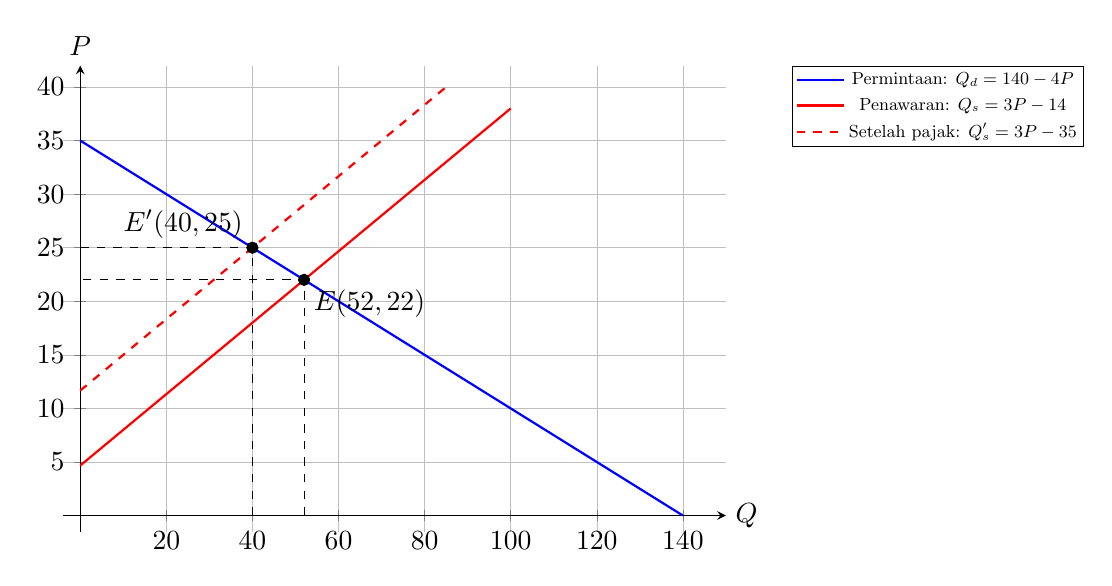
\begin{tikzpicture}
                    \begin{axis}[
        axis lines = middle,
        xlabel = $x$,
        ylabel = {$y$},
        grid=both,
        grid style={line width=.1pt, draw=gray!10},
        major grid style={line width=.2pt,draw=gray!50},
        x label style={anchor=west}, % label x ke kanan
        y label style={anchor=south}, % label y ke atas
        samples=200,
        legend style={
                at={(1.1,1)},
                anchor=north west,
                font=\small,         % mengecilkan ukuran font
                row sep=1pt,         % jarak antar baris legend
                inner sep=1pt,       % margin dalam kotak legend
                nodes={scale=0.7}    % skalakan isi legend
            },
        xlabel = $Q$,
        ylabel = {$P$},
        xtick={0,20,...,140},
        ytick={0,5,...,40},
        xmin=-4, xmax=150,
        ymin=-1.5, ymax=42,
        width=10cm,
        height=7.5cm
    ]
\addplot[domain=0:140, color=blue, thick, samples=2] {(140-x)/4};
\addlegendentry{Permintaan: $Q_d=140-4P$}
\addplot[domain=0:100, color=red, thick, samples=2] {(x+14)/3};
\addlegendentry{Penawaran: $Q_s=3P-14$}
\addplot[domain=0:85, color=red, thick, dashed, samples=2] {(x+35)/3};
\addlegendentry{Setelah pajak: $Q_s'=3P-35$}
\draw[fill=black] (52,22) circle (2pt) node[below right] {$E(52,22)$};
\draw[fill=black] (40,25) circle (2pt) node[above left] {$E'(40,25)$};
\draw[dashed] (52,0) -- (52,22) -- (0,22);
\draw[dashed] (40,0) -- (40,25) -- (0,25);
\end{axis}
                \end{tikzpicture}
            \end{center}
        \end{enumerate}
    }
    \end{jawab}
\end{enumerate}

\newpage

% includepdf hanya dijalankan pada job utama (bukan saat externalize gambar TikZ)
\ifx\pgfactualjobname\tikzexternalrealjob
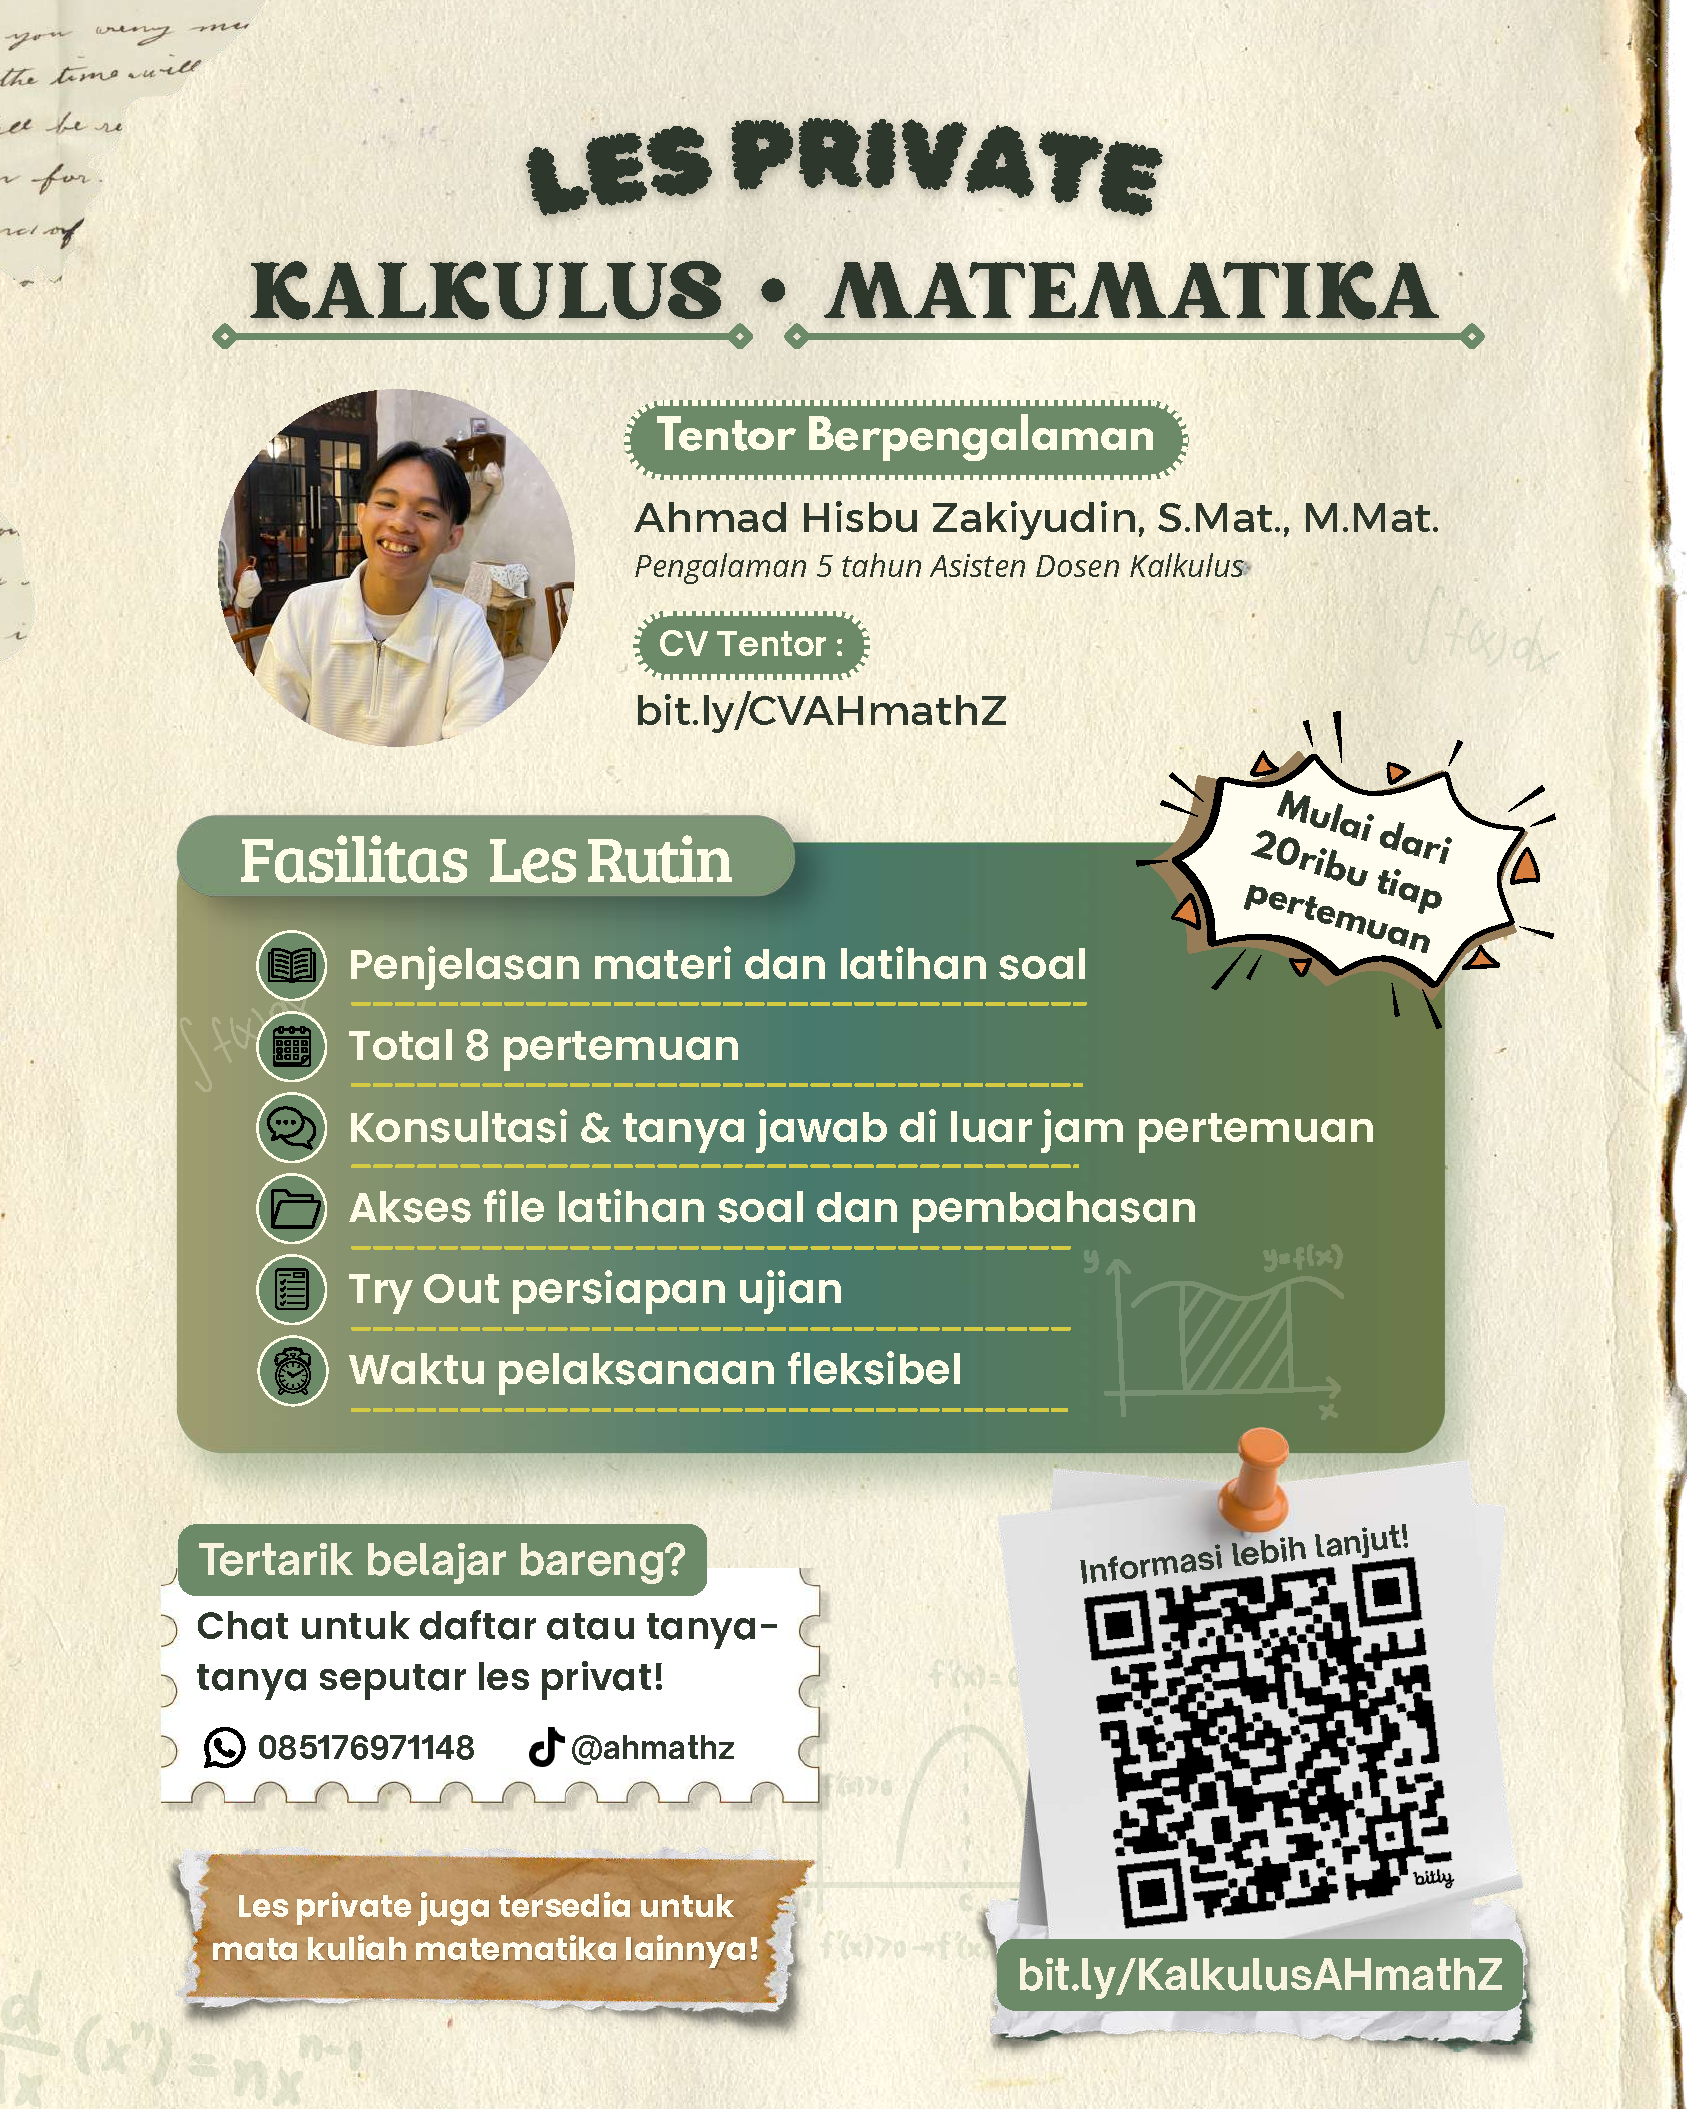
\includepdf[pages=-]{../ETS_Kalkulus_1_Th_2025-2026/les.pdf}
\fi

\end{document}
